% Define the page style
\fancypagestyle{chapterstyle}{
   \fancyhead[L]{\nouppercase{\rightmark}}
   \fancyhead[R]{Projet de fin d'études 2023-2024}
   \fancyfoot[C]{\vspace{20pt}\thepage} % Adjust the vertical space here
   \setlength{\headheight}{20pt}
   \setlength{\footskip}{30pt} % Adjust the value as needed
}





\chapter{Implémentation et Validation}
\pagestyle{chapterstyle}


\newpage
\vspace{1cm}

\section{Introduction}
%  Cette phase 
% consiste à concrétiser le modèle conceptuel précédemment établi 
% en composants logiciels formant notre système, puis à vérifier 
% leur bon fonctionnement. Dans ce chapitre, nous allons présenter 
% de manière succincte les différents outils que nous avons utilisés 
% tout au long du développement et de la validation de notre 
% application.
Dans ce chapitre, nous présentons de manière concise les différents 
outils et technologies utilisés tout au long du développement et de la validation de notre 
application, accompagnés des captures d'écran illustrant leur mise en œuvre.



\section{Outils et technologies de développement}
\subsection{Outils de conception}

\large 
\textbf{Figma}

\begin{figure}[htbp]
   \centering
   
\includegraphics[scale=0.03]{Images/figma.png} 
   \caption{Logo Figma\cite{figma}}
   \label{fig:figma}
\end{figure}
Figma est un outil de design collaboratif en ligne pour la 
création d'interfaces utilisateur. Il permet de créer des 
maquettes et des prototypes interactifs, facilitant la 
collaboration en temps réel\cite{figma}. C'est l'outil que nous avons utilisé 
pour créer les maquettes de notre projet.
\newline

\large 
\textbf{Lucidchart}
\begin{figure}[htbp]
   \centering
   
\includegraphics[scale=0.2]{Images/lucid.jpeg} 
   \caption{Logo Lucidchart\cite{LucidChart}}
   \label{fig:lucid}
\end{figure}

Lucidchart est un outil en ligne pour créer et partager des 
diagrammes et des visualisations de données. Il permet de 
dessiner des diagrammes de flux, des organigrammes, des cartes 
conceptuelles, et bien d'autres schémas \cite{LucidChart}. Cet outil a été utilisé pour
la conception des différents diagrammes de cas d'utilisation, de classe et de séquence.

\subsection{Environnement de développement}
\large 
\textbf{Visual Studio Code}

\begin{figure}[htbp]
   \centering
   
\includegraphics[scale=0.06]{Images/vs.png} 
   \caption{Logo Visual Stduio Code\cite{vsCode}}
   \label{fig:vscode}
\end{figure}

Visual Studio Code est un éditeur de texte open source,
 gratuit et multiplateforme (Windows, Mac et Linux), 
 développé par Microsoft\cite{vsCode}. Cet environnement de développement 
 a été utilisé pour développer la partie frontend du projet, gérer la console Git et rédiger le rapport en utilisant l'extension LaTeX Workshop.
\newline

\large 
\textbf{4D Client}

\begin{figure}[htbp]
   \centering
   
\includegraphics[scale=0.2]{Images/4dcl.png} 
   \caption{Logo 4D Client\cite{4d}}
   \label{fig:4dcl}
\end{figure}

4D vous permet de construire des applications client-serveur 
personnalisées qui sont homogènes, multiplateformes et avec 
une option de mise à jour automatique. Les applications 
client et serveur sont configurées dans la page Client/Serveur 
de la boîte de dialogue Construire une application \cite{4d}.
Cet outil nous a servi pour developpe la partie backend du projet 
en se concentrant sur le volet metier du projet, il facilite la gestion
des données et la mise en place de la base de données graphique.
\newline

\large 
\textbf{4D Serveur}

\begin{figure}[htbp]
   \centering
   
\includegraphics[scale=0.2]{Images/4dsrv.png} 
   \caption{Logo 4D Serveur\cite{4d}}
   \label{fig:4dsrv}
\end{figure}

4D Server est un composant logiciel de la plateforme de développement 
4D qui permet le déploiement et la gestion
d’applications client-sebrveur. Il offre un environnement robuste 
et évolutif pour héberger des applications 4D, 
permettant à plusieurs utilisateurs d’y accéder et d’interagir avec
l’application simultanément. 4D Server agit comme un hub centralisé, 
gérant le stockage des données, le traitement et la communication entre 
le serveur et les applications clientes connectées. Il prend en charge 
des fonctionnalités telles que l’accès simultané aux données partagées, 
la gestion des transactions, les contrôles de sécurité et la collaboration
multi-utilisateur\cite{4d}.
\newline

Ces caractéristiques du serveur 4D permettent de garantir les exigences non fonctionnelles mentionnées précédemment : la disponibilité, la performance et l'évolutivité. 
\newline

\large 
\textbf{Postman}

\begin{figure}[htbp]
   \centering
   
\includegraphics[scale=0.4]{Images/postman.png} 
   \caption{Logo postman\cite{Postman}}
   \label{fig:postman}
\end{figure}

Postman fournit une interface conviviale où les développeurs 
peuvent spécifier les paramètres de requête, les entêtes, 
les corps de requête, les méthodes HTTP, etc. Ils peuvent 
également inspecter les réponses des serveurs, valider les 
résultats et effectuer des tests automatisés pour s’assurer que 
l’API fonctionne correctement\cite{Postman}. Le rôle de Postman 
dans notre projet est indispensable, car il permet de vérifier 
le bon fonctionnement de la partie backend et de valider les 
données envoyées et reçues entre le serveur et le client.
\newline

\large 
\textbf{GitLab}

\begin{figure}[htbp]
   \centering
   
\includegraphics[scale=0.6]{Images/gitlab.jpg} 
   \caption{Logo GitLab\cite{gitlab}}
   \label{fig:gitlab}
\end{figure}
GitLab est une plateforme DevOps complète proposée sous la forme 
d’une application unique. Elle révolutionne le développement, 
la sécurité, l’exploitation et la collaboration entre les équipes. 
Créez, testez et déployez des logiciels plus rapidement en 
n’utilisant qu’une seule solution. GitLab nous a permis de collaborer tout au long du projet pour gérer les versions, les modifications et les mises à jour du code.
\subsection{Langages de développement}
\large 
\textbf{4D}

\begin{figure}[htbp]
   \centering
   
\includegraphics[scale=0.8]{Images/logo-4d.jpg} 
   \caption{Logo 4D\cite{4d}}
   \label{fig:4D}
\end{figure}
Le langage 4D est un langage de programmation spécifique à la
plateforme utilisé dans l’environnement de développement 4D pour
créer des applications professionnelles et des bases de données. 
Il est conçu pour simplifier le développement d’applications 
en fournissant des fonctionnalités spécifiques à la gestion des 
données et des interfaces utilisateur\cite{4d}. 
\newline

Nous avons utilisé le langage 4D principalement pour l'insertion de données de type objet. Ce langage nous a également permis de créer des méthodes et des classes selon les besoins du projet. Grâce à ses capacités avancées de manipulation des objets, 4D a facilité la structuration et la gestion des données complexes. En outre, la possibilité de définir des méthodes et des classes a offert une grande flexibilité dans l'implémentation de la logique métier, rendant le développement plus modulable et maintenable.
\newline

\large 
\textbf{TypeScript}
\begin{figure}[h]
   \centering
   
\includegraphics[scale=0.05]{Images/ts.png} 
   \caption{Logo TypeScript\cite{TypeScript}}
   \label{fig:ts}
\end{figure}

TypeScript, développé par Microsoft, est un surensemble de 
JavaScript qui ajoute des types statiques, permettant de
détecter les erreurs dès la phase de développement. Il compile 
en JavaScript standard et est compatible avec tous les 
navigateurs. TypeScript offre des fonctionnalités avancées 
comme les interfaces, les énumérations et les génériques, 
et bénéficie d'un excellent support des outils de développement, 
facilitant l'auto-complétion et la refactorisation\cite{TypeScript}. 
Ces caractéristiques en 
font un choix idéal pour les applications à grande échelle 
où la qualité et la maintenabilité du code sont cruciales, 
ce qui nous a conduit à l'adopter pour notre projet évolutif.
\newline

\large
\textbf{HTML}
\begin{figure}[htbp]
   \centering
   
\includegraphics[scale=0.15]{Images/html.png} 
   \caption{Logo HTML\cite{HTML}}
   \label{fig:html}
\end{figure}

HTML est un langage de balisage conçu pour représenter les pages
 web. C’est un langage permettant d’écrire de l’hypertexte, 
 d’où son nom. HTML permet également de structurer sémantiquement 
 et logiquement et de mettre en forme le contenu des pages, 
 d’inclure des ressources multimédias dont des images, des 
 formulaires de saisie et des programmes informatiques\cite{HTML}.
\newline

\subsection{Frameworks}
\large
\textbf{React}
\begin{figure}[htbp]
   \centering
   
\includegraphics[scale=0.1]{Images/react.png} 
   \caption{Logo React\cite{React}}
   \label{fig:react}
\end{figure}

React est une bibliothèque JavaScript frontale open source 
permettant de créer des interfaces utilisateur ou des composants 
d'interface utilisateur. Il est maintenu par Facebook et une 
communauté de développeurs individuels et d'entreprises. 
React peut être utilisé comme base dans le développement 
d'applications monopages ou mobiles. Nous avons choisi 
d'utiliser ce framework dans notre projet en raison de sa 
capacité à créer des interfaces utilisateur dynamiques et 
réactives, de sa gestion efficace de l'état et des mises à 
jour en temps réel, ainsi que de la réutilisabilité de ses 
composants\cite{React}. Ces caractéristiques facilitent la maintenance, 
la scalabilité et l'évolution de notre application, 
répondant ainsi aux besoins de notre projet.
\newline

\large
\textbf{Tailwind}
\begin{figure}[htbp]
   \centering
   
\includegraphics[scale=0.5]{Images/tailwind.png} 
   \caption{Logo Tailwind\cite{Tailwind}}
   \label{fig:tailwind}
\end{figure}

Tailwind est un framework CSS qui fournit un catalogue complet 
de classes et d’outils CSS permettant de styliser facilement un 
site web ou une application. Nous avons choisi d'utiliser 
Tailwind dans notre projet en raison de plusieurs avantages 
clés. Premièrement, Tailwind facilite une conception rapide et 
efficace grâce à ses classes utilitaires préconçues, éliminant 
le besoin d'écrire des CSS personnalisés pour chaque élément. 
Deuxièmement, il offre une grande flexibilité et permet de créer 
des designs réactifs et cohérents. Enfin, Tailwind améliore 
la maintenabilité du code en gardant les styles directement dans 
les classes HTML, ce qui simplifie la gestion des styles et 
réduit les conflits CSS\cite{Tailwind}. Ces caractéristiques nous ont permis de 
développer une interface utilisateur esthétique et fonctionnelle 
tout en accélérant le processus de développement.
\newline

\large
\textbf{Axios}
\begin{figure}[h]
   \centering
   
\includegraphics[scale=0.5]{Images/axios.png}
   \caption{Logo Axios\cite{Axios}}
\end{figure}

Dans le contexte de notre projet, nous avons intégré Axios en 
raison de sa capacité à simplifier la gestion des requêtes HTTP 
entre notre frontend basé sur React et notre backend. Axios nous 
permet de réaliser des appels API de manière efficace et fiable, 
en utilisant une syntaxe claire et intuitive. Cela facilite 
l'intégration des fonctionnalités d'interaction avec le serveur, 
comme la récupération et l'envoi de données dynamiques, 
essentielles pour assurer la réactivité et la performance de 
notre application. En utilisant Axios avec React, nous avons 
pu maintenir un flux de données fluide et sécurisé, répondant 
ainsi aux exigences de notre projet en termes de communication 
client-serveur.
\newline

\large
\textbf{Cypress}
\begin{figure}[htbp]
   \centering
   
\includegraphics[scale=0.6]{Images/cy.jpg} 
   \caption{Logo Cypress\cite{Cypress}}
   \label{fig:cypress}
\end{figure}

Cypress est un framework de tests bout-en-bout open source qui 
s'intègre parfaitement avec notre pile technologique, notamment 
React et Tailwind CSS. Nous l'avons utilisé pour garantir le bon 
fonctionnement et la bonne stylisation de nos composants 
frontaux. Cypress facilite l'écriture et la maintenance des 
tests grâce à son support pour JavaScript moderne et son 
exécution directe dans le navigateur. Ses outils de débogage 
et de visualisation des tests nous permettent de résoudre 
rapidement les problèmes\cite{Cypress}. En automatisant nos tests avec Cypress, 
nous avons assuré une couverture complète des fonctionnalités 
critiques et une détection précoce des régressions, maintenant 
ainsi la qualité de notre code.

% travail realise
\section{Captures d'écran}
Cette section présente des captures d'écran de diverses interfaces de notre application, 
accompagnées de descriptions  détaillées.  Chaque  capture  illustre une interface 
spécifique de l'application et met en avant les fonctionnalités principales disponibles. 
% Les descriptions fournissent des informations sur la disposition de l'interface, 
% les boutons et les menus pertinents, ainsi que sur les actions que les utilisateurs 
% peuvent réaliser.
\subsection{Page d'accueil}

La page  d’accueil est  conçue pour offrir une expérience utilisateur intuitive et 
informative. En haut une  barre  de navigation avec le logo de l’application et 
des liens vers les principales sections comme le bouton “sign in” qui permet l’utilisateur de  
naviguer vers la page d’authentification. La section principale attire immédiatement 
l’attention avec un message accrocheur et une illustration attrayante, présentant 
l'objectif de la  plateforme. Les catégories d’emploi sont mises en  avant. 
Une section de guide des utilisateurs à travers des étapes simples de candidature. 
Un appel à l’action “Ready to start ?”  encourage l'engagement, en  redirigeant 
l’utilisateur vers la page d’inscription.  
\begin{figure}[htbp]
   \centering
   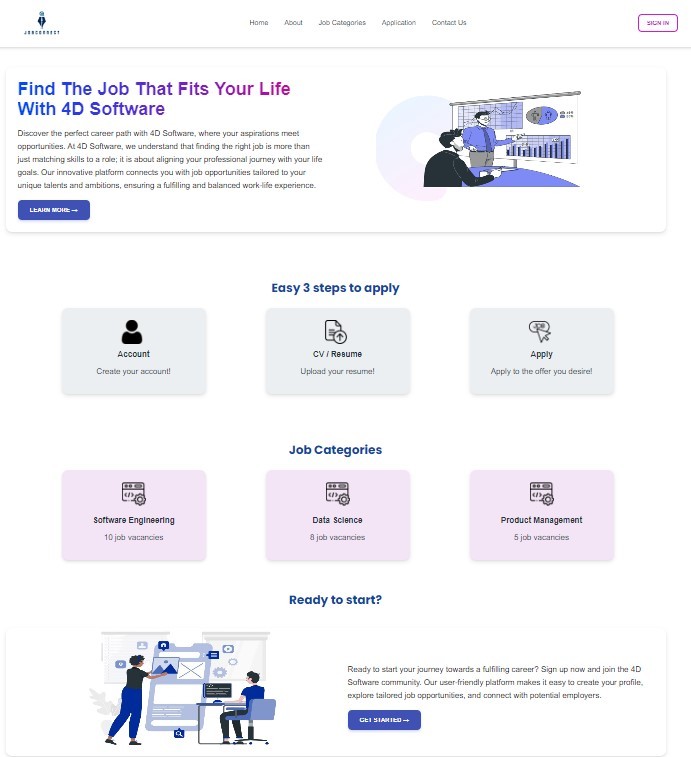
\includegraphics[scale=0.7]{screens/accueil2.jpg} 
   \caption{Page d'accueil}
   \label{fig:accueil}
\end{figure}

\vspace{2cm}
\subsection{Authentification}
En cliquant le bouton “Sign In”, l’utilisateur sera redirigé vers la page d’authentification. 
Les utilisateurs peuvent saisir leurs  informations  d’identification, 
leur email et leur mot de passe, dans les champs correspondants. 
 Si les données saisies sont 
valides, l’utilisateur va accéder à son espace personnel, en fonction de 
son rôle.
\newline
\begin{figure}[htbp]
   \centering
   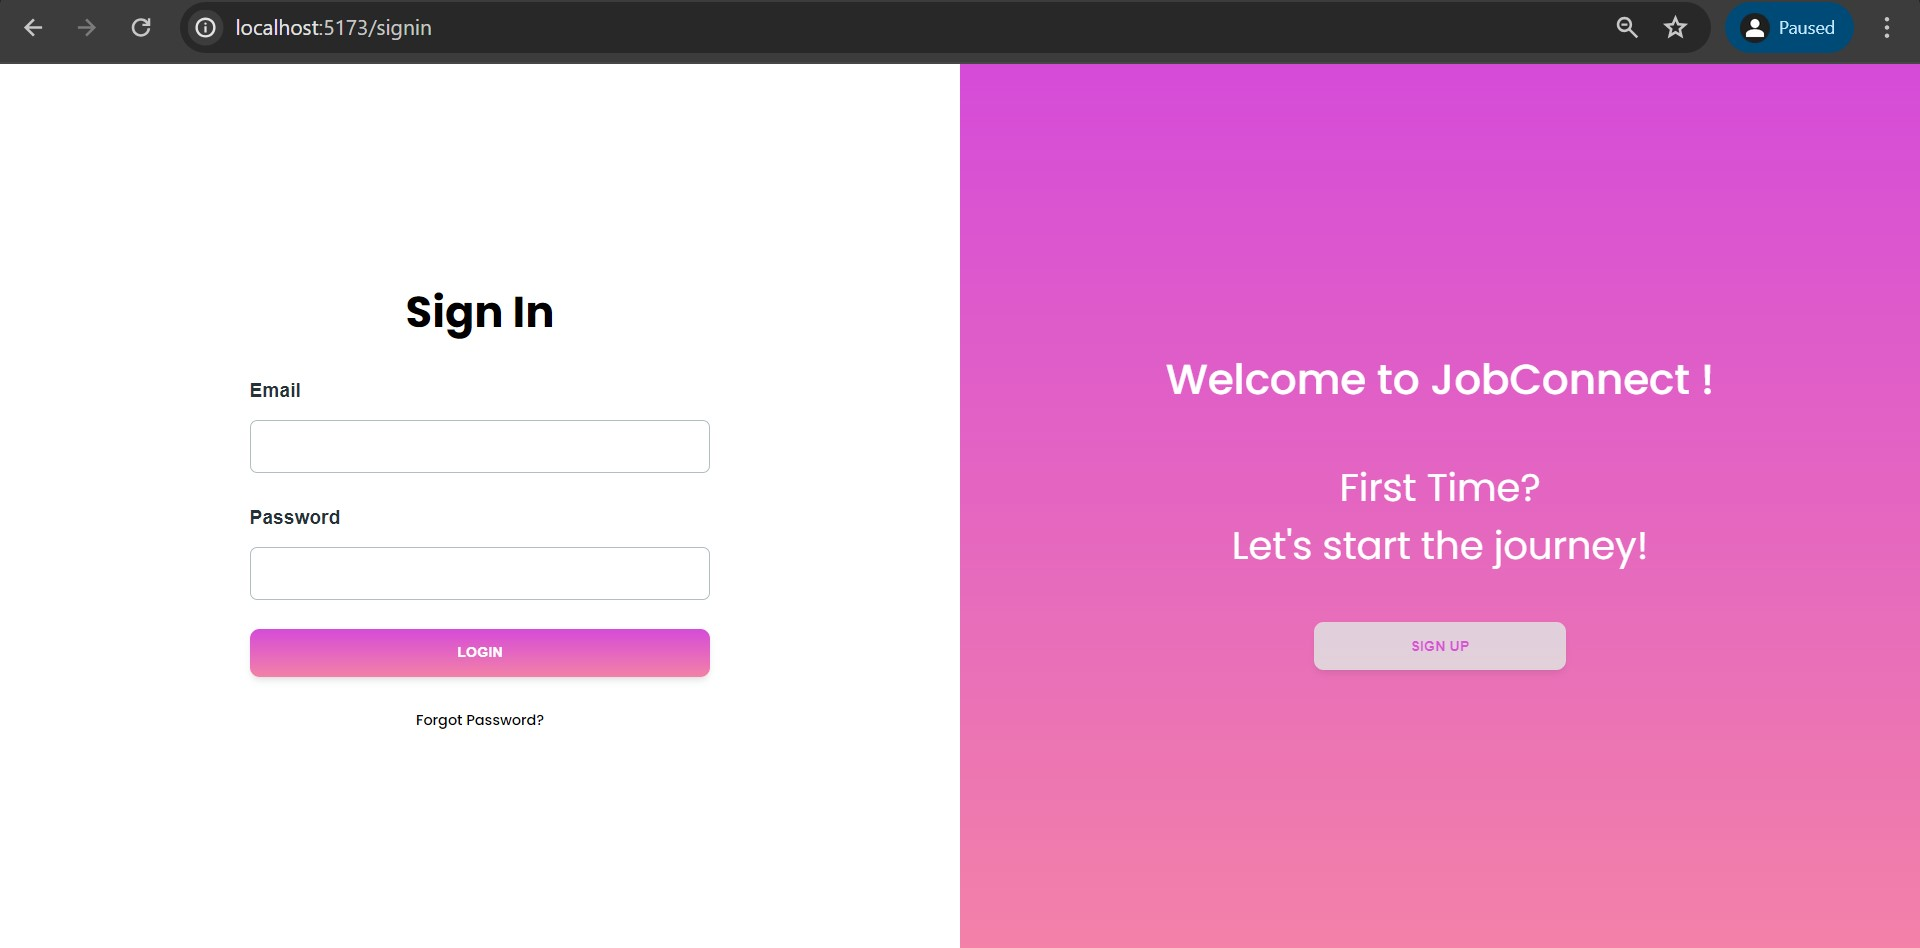
\includegraphics[scale=0.5]{screens/signin.jpg} 
   \caption{Page d'authentification}
   \label{fig:accueil}
\end{figure}

Si les informations sont incorrectes, un message d’erreur "Wrong Email or Password" 
sera affiché. Si l’utilisateur oublie son mot de passe, il peut le réinitialiser en 
cliquant sur la fonctionnalité "Forgot Password  ?",  qui  le redirigera vers une autre 
page illustrée par la figure \ref{fig:forgotPass}. Sur cette page, il pourra remplir 
son  email. Une  fois soumis, l'application vérifiera immédiatement la présence de 
l'adresse email dans sa base de données. Si elle n'est pas trouvée, un message d’erreur 
sera affiché. 
\newline
\begin{figure}[htbp]
   \centering
   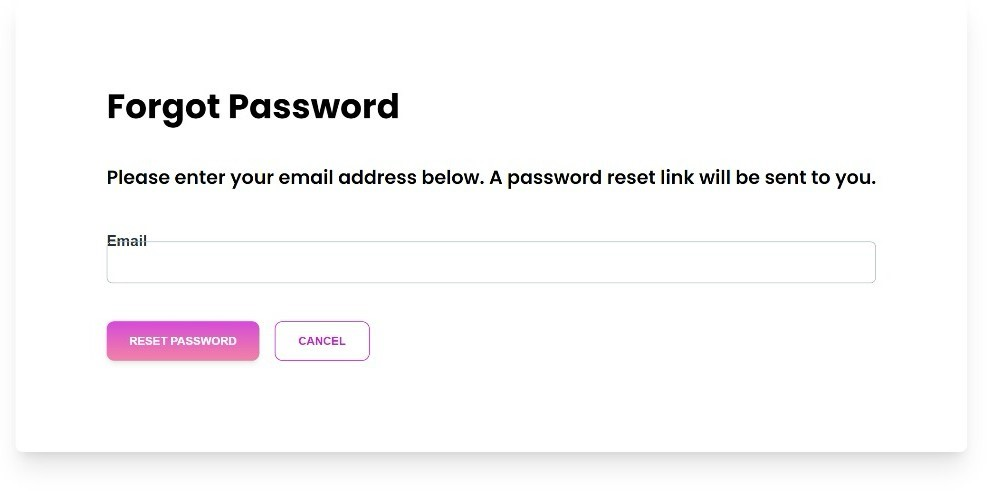
\includegraphics[scale=0.6]{screens/forgot.jpg} 
   \caption{Mot de passe oublié}
   \label{fig:forgotPass}
\end{figure}
\vspace{5cm}

% Sinon, si  l'email est  trouvé, un  courriel sera envoyé à l'adresse fournie via la 
% méthode POST, contenant le  nouveau mot de  passe, comme illustré dans la figure.
Sinon, si l'adresse mail est trouvée, l'utilisateur recevra
un email de réinitialisation de mot de passe dans sa boite mail, comme illustré dans la figure \ref{fig:mailPass}.

\begin{figure}[htbp]
   \centering
   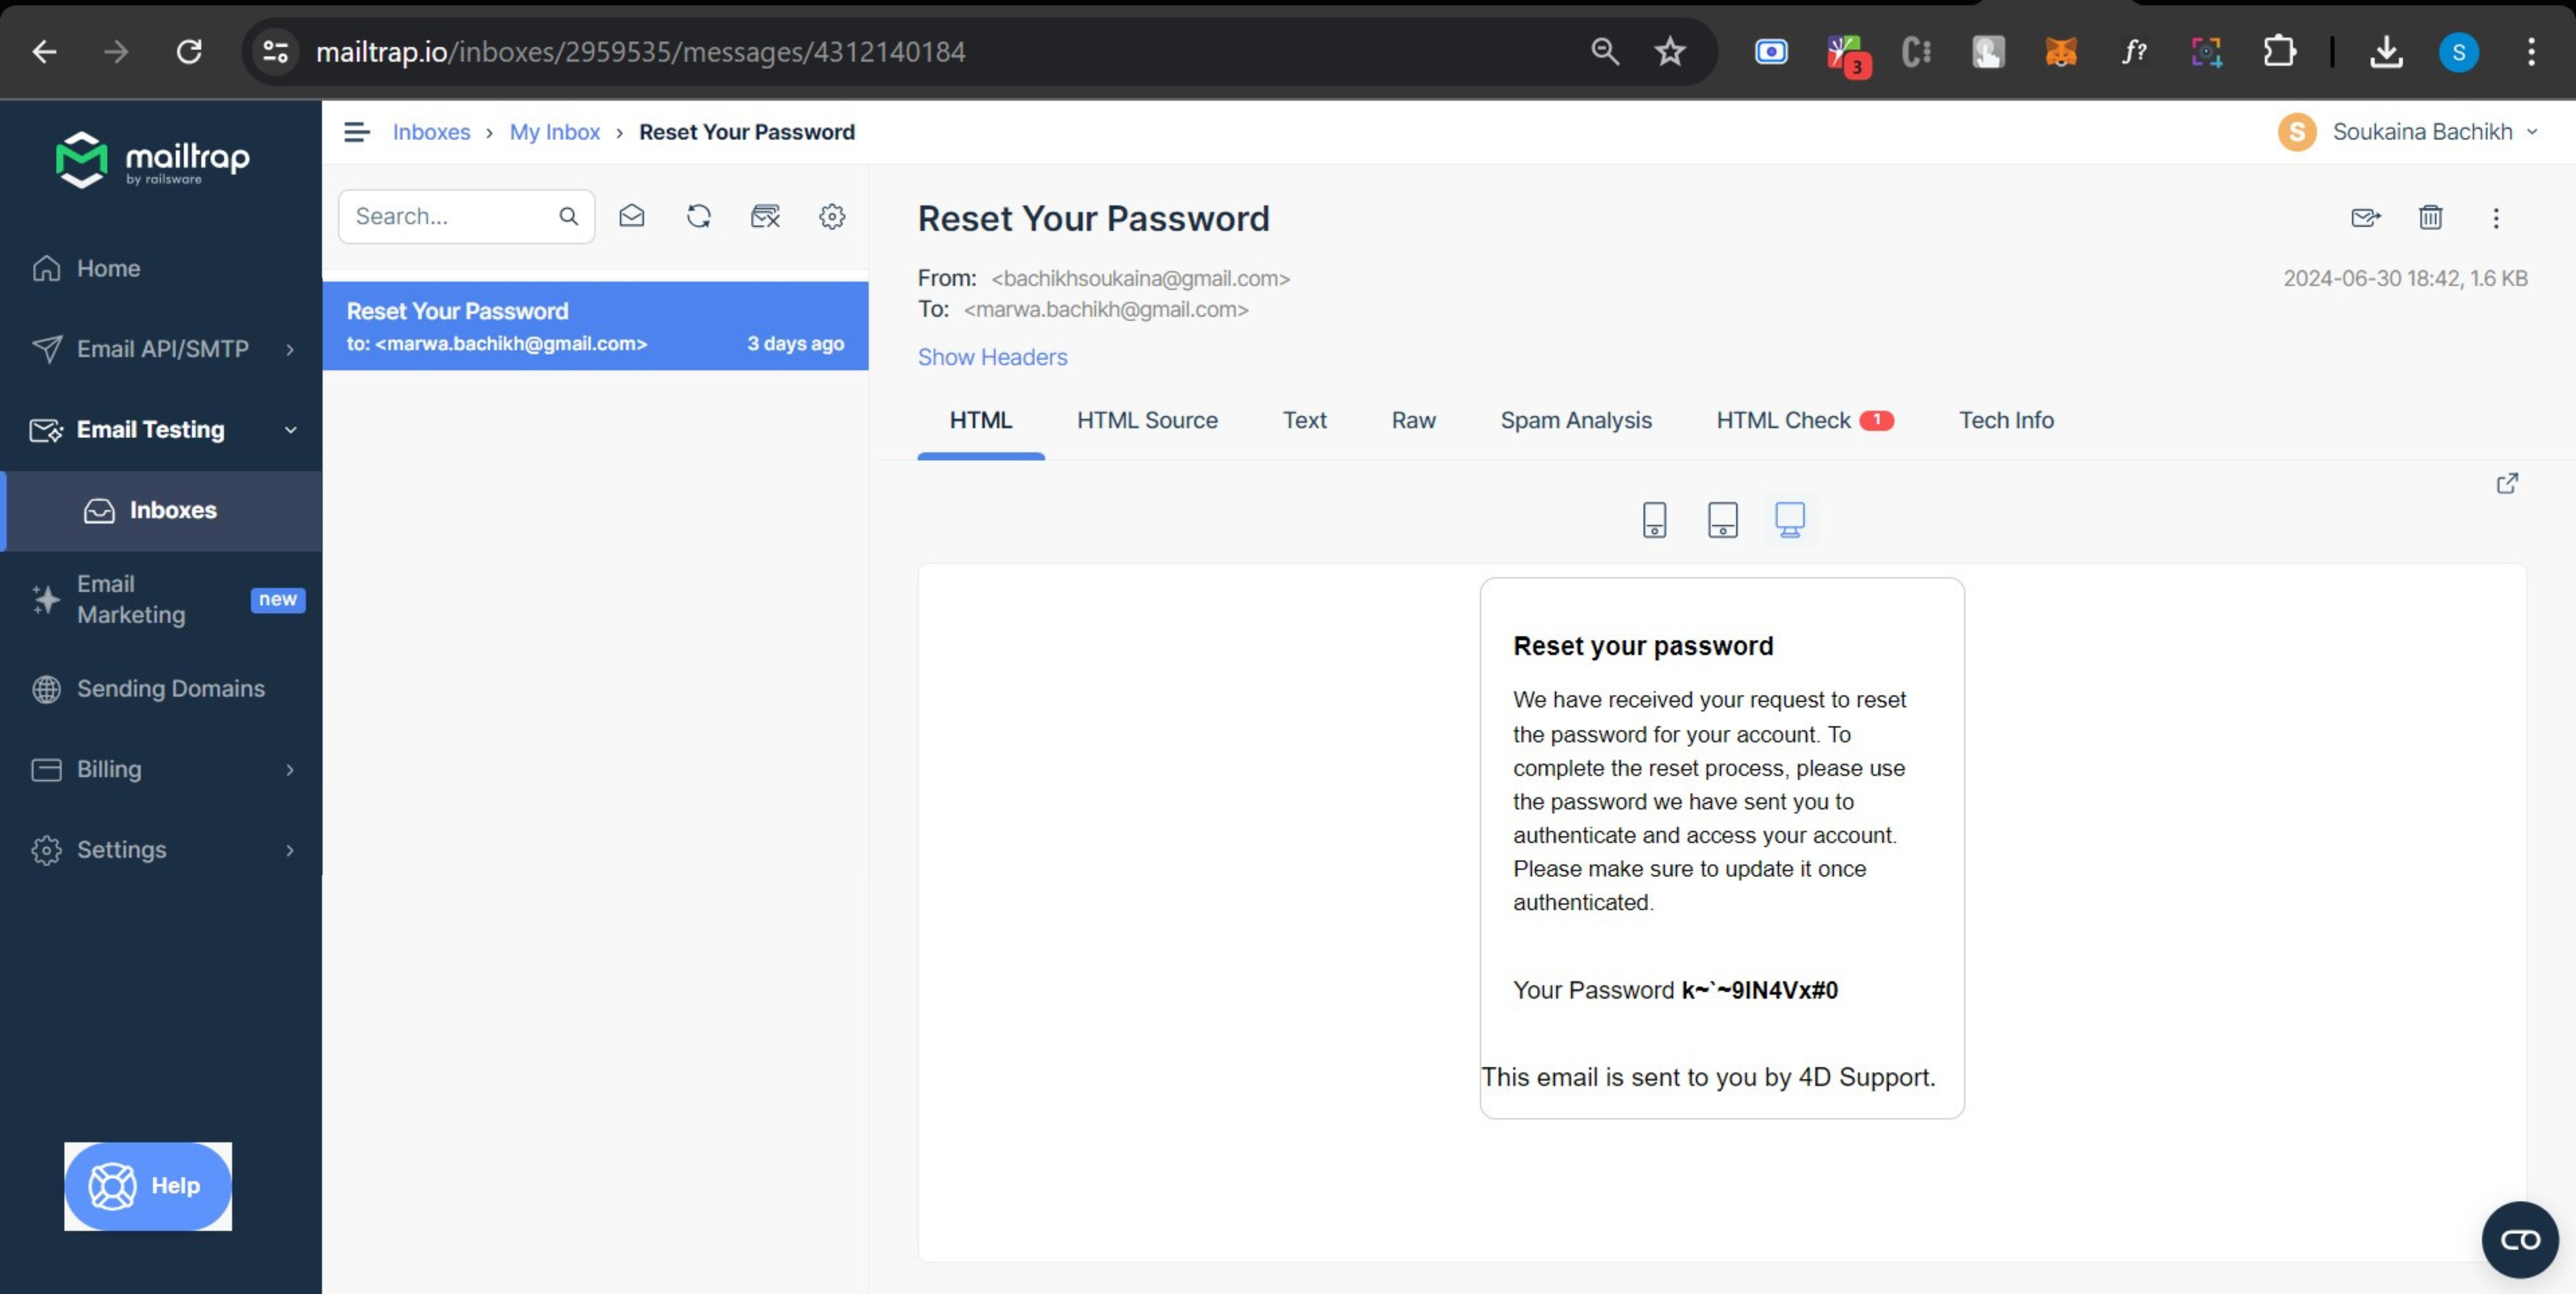
\includegraphics[scale=0.26]{screens/mailForgot.png} 
   \caption{Exemple d'un email pour réintialiser le mot de passe}
   \label{fig:mailPass}
\end{figure}

\subsection{Espace Candidat}
\subsubsection{La page d’inscription}
Le candidat peut accéder au formulaire d’inscription à partir du bouton 
“Ready to start?” ou le bouton “Sign up” de la page d’authentification. 
Ce forumulaire comme il est représenté sur la figure \ref{fig:singup}. 
À droite, la section pour l'inscription comporte des champs de 
formulaire pour entrer des informations personnelles, 
y compris le prénom, le nom, le courriel, le mot de  passe, et  
le numéro de téléphone. En bas, un bouton "REGISTER” permet de finaliser 
l'inscription. Juste en dessous, il y a un lien "Already have an account ? Sign In" 
pour rediriger les utilisateurs vers la page de connexion s’ils ont déjà 
un compte.

\begin{figure}[htbp]
   \centering
   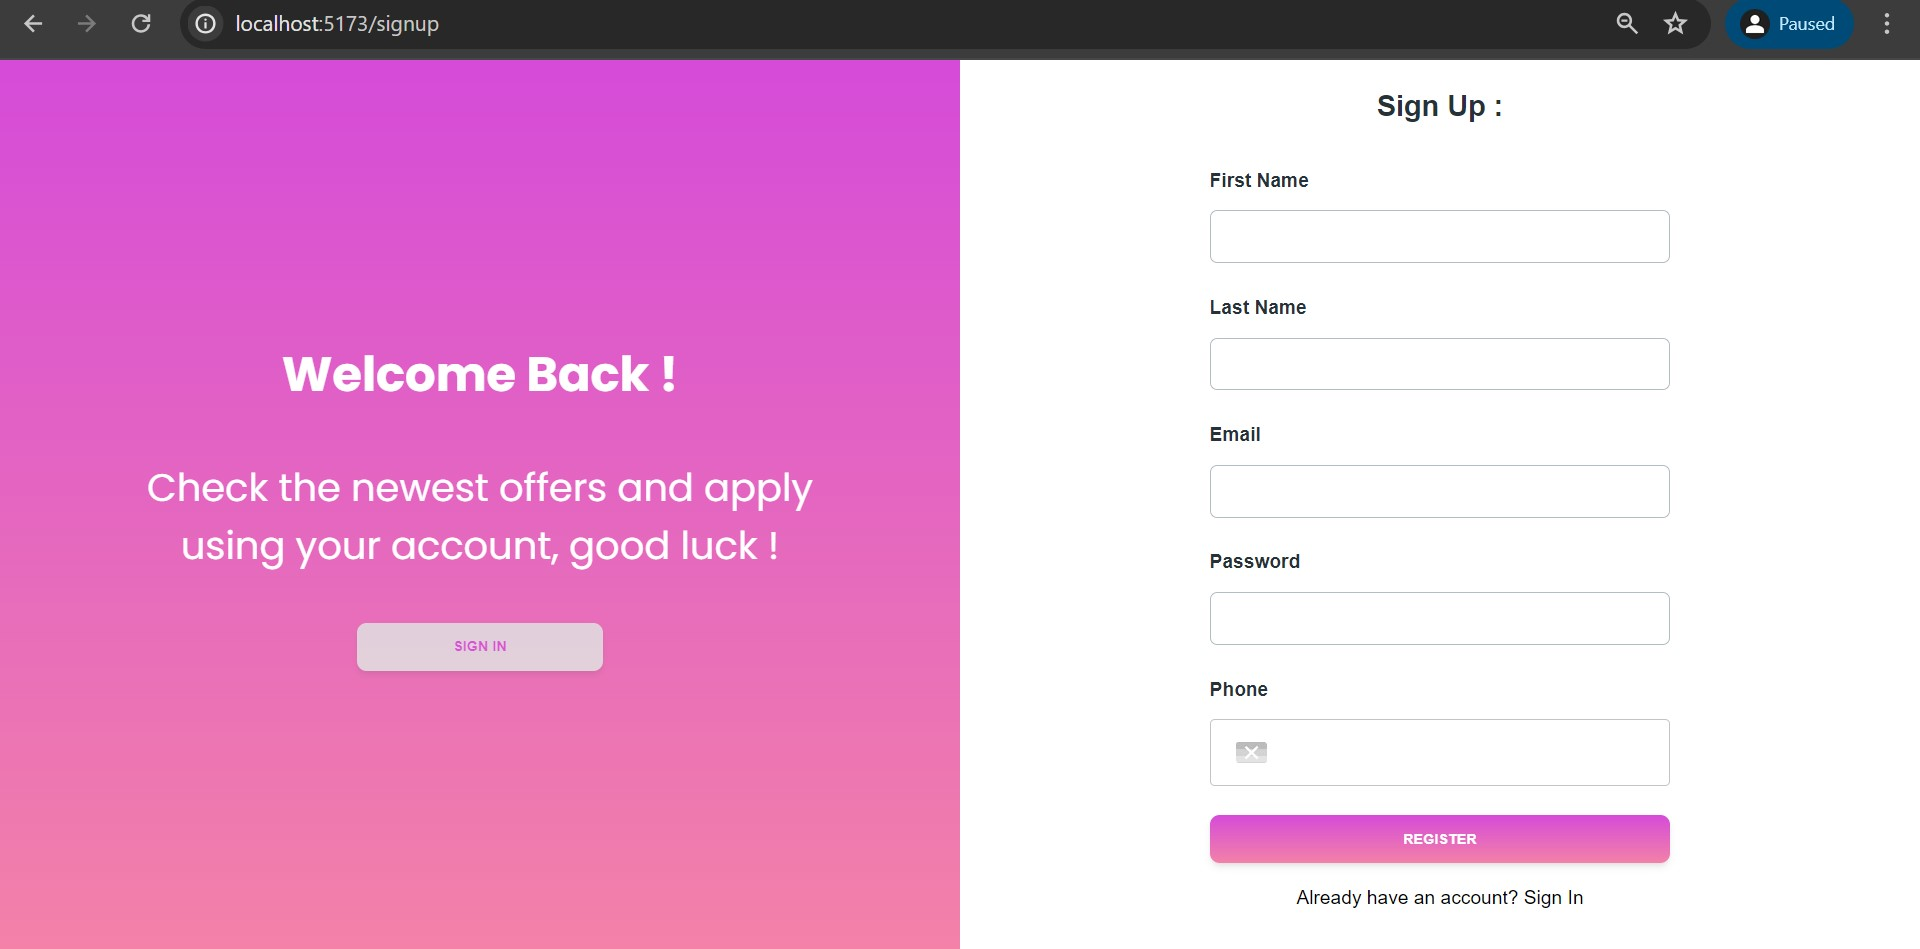
\includegraphics[scale=0.4]{screens/signup.jpg} 
   \caption{Page d'inscription}
   \label{fig:singup}
\end{figure}

\subsubsection{Profil}
Après l'authentification, chaque utilisateur se voit attribuer 
un  rôle (candidat, recruteur ou administrateur),  qui  
détermine  l'accès  à son  espace dédié. Prenons d'abord le cas 
où l'utilisateur est un candidat : il est redirigé directement 
vers son profil, comme illustré dans la figure \ref{fig:profile}.
\newline

Dans la première section de son profil, le  candidat peut mettre 
à jour sa photo et ses informations personnelles. Dans la 
deuxième section, il  peut ajouter ou mettre à jour son CV et 
sa lettre  de  motivation.  Enfin,  dans  la  dernière section, 
il a la possibilité de réinitialiser son mot de passe pour la 
plateforme.
\newline


\begin{figure}[htbp]
   \centering
   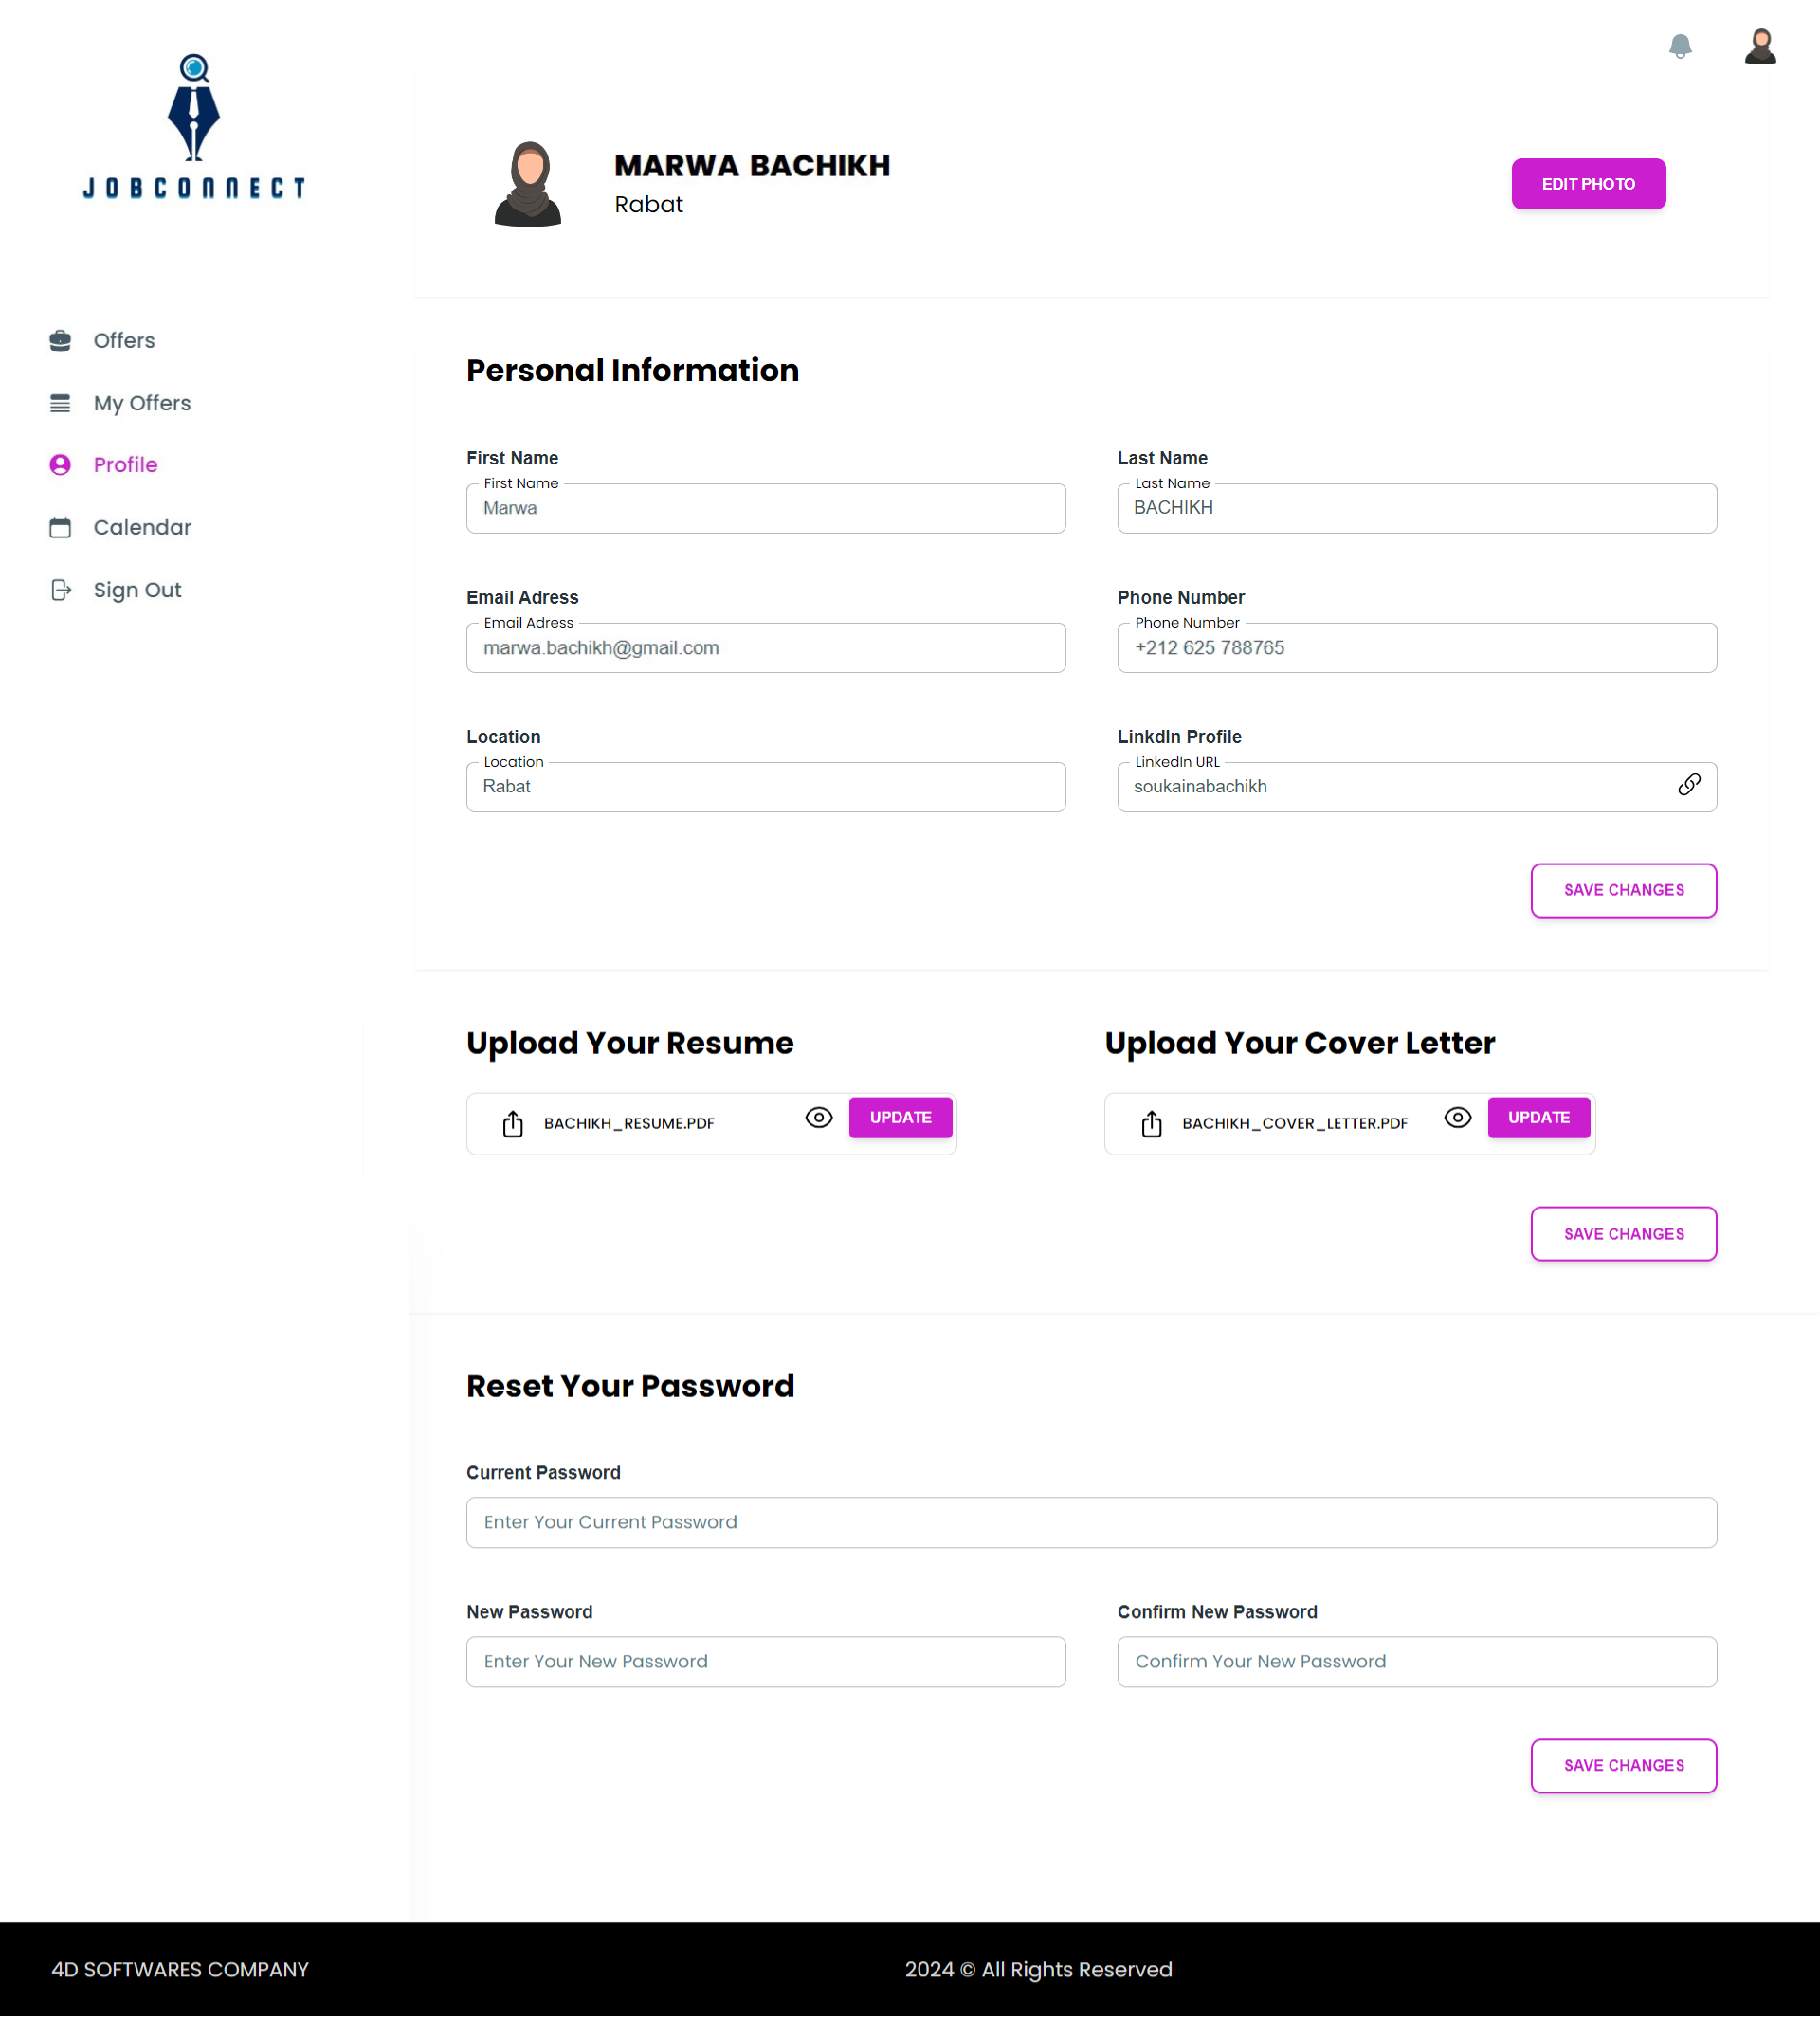
\includegraphics[scale=0.3]{screens/profill.png} 
   \caption{Profil}
   \label{fig:profile}
\end{figure}

\vspace{6cm}

\subsubsection{Postuler à une offre}
En naviguant via le menu de gauche, un simple clic sur le 
bouton "Offres" conduit à la page représentée par la figure \ref{fig:listOffers}.  
Cette  page  présente plusieurs cartes, chacune décrivant une  
offre d'emploi active, et  publiée par un 
recruteur. Chaque carte comprend les détails suivants : 
le titre du poste, la localisation, une description 
du poste, le  type de  contrat (stage, emploi, etc.), et 
le mode de travail (présentiel, télétravail, ou hybride). En haut 
de la page, un menu permet de filtrer les offres d'emploi par 
domaine, tel que DevOps, Data science, et software engineering.
\newline

Chaque page affiche jusqu'à 6 cartes,  avec  une  fonction  de  pagination pour accéder aux offres suivantes.
\begin{figure}[htbp]
   \centering
   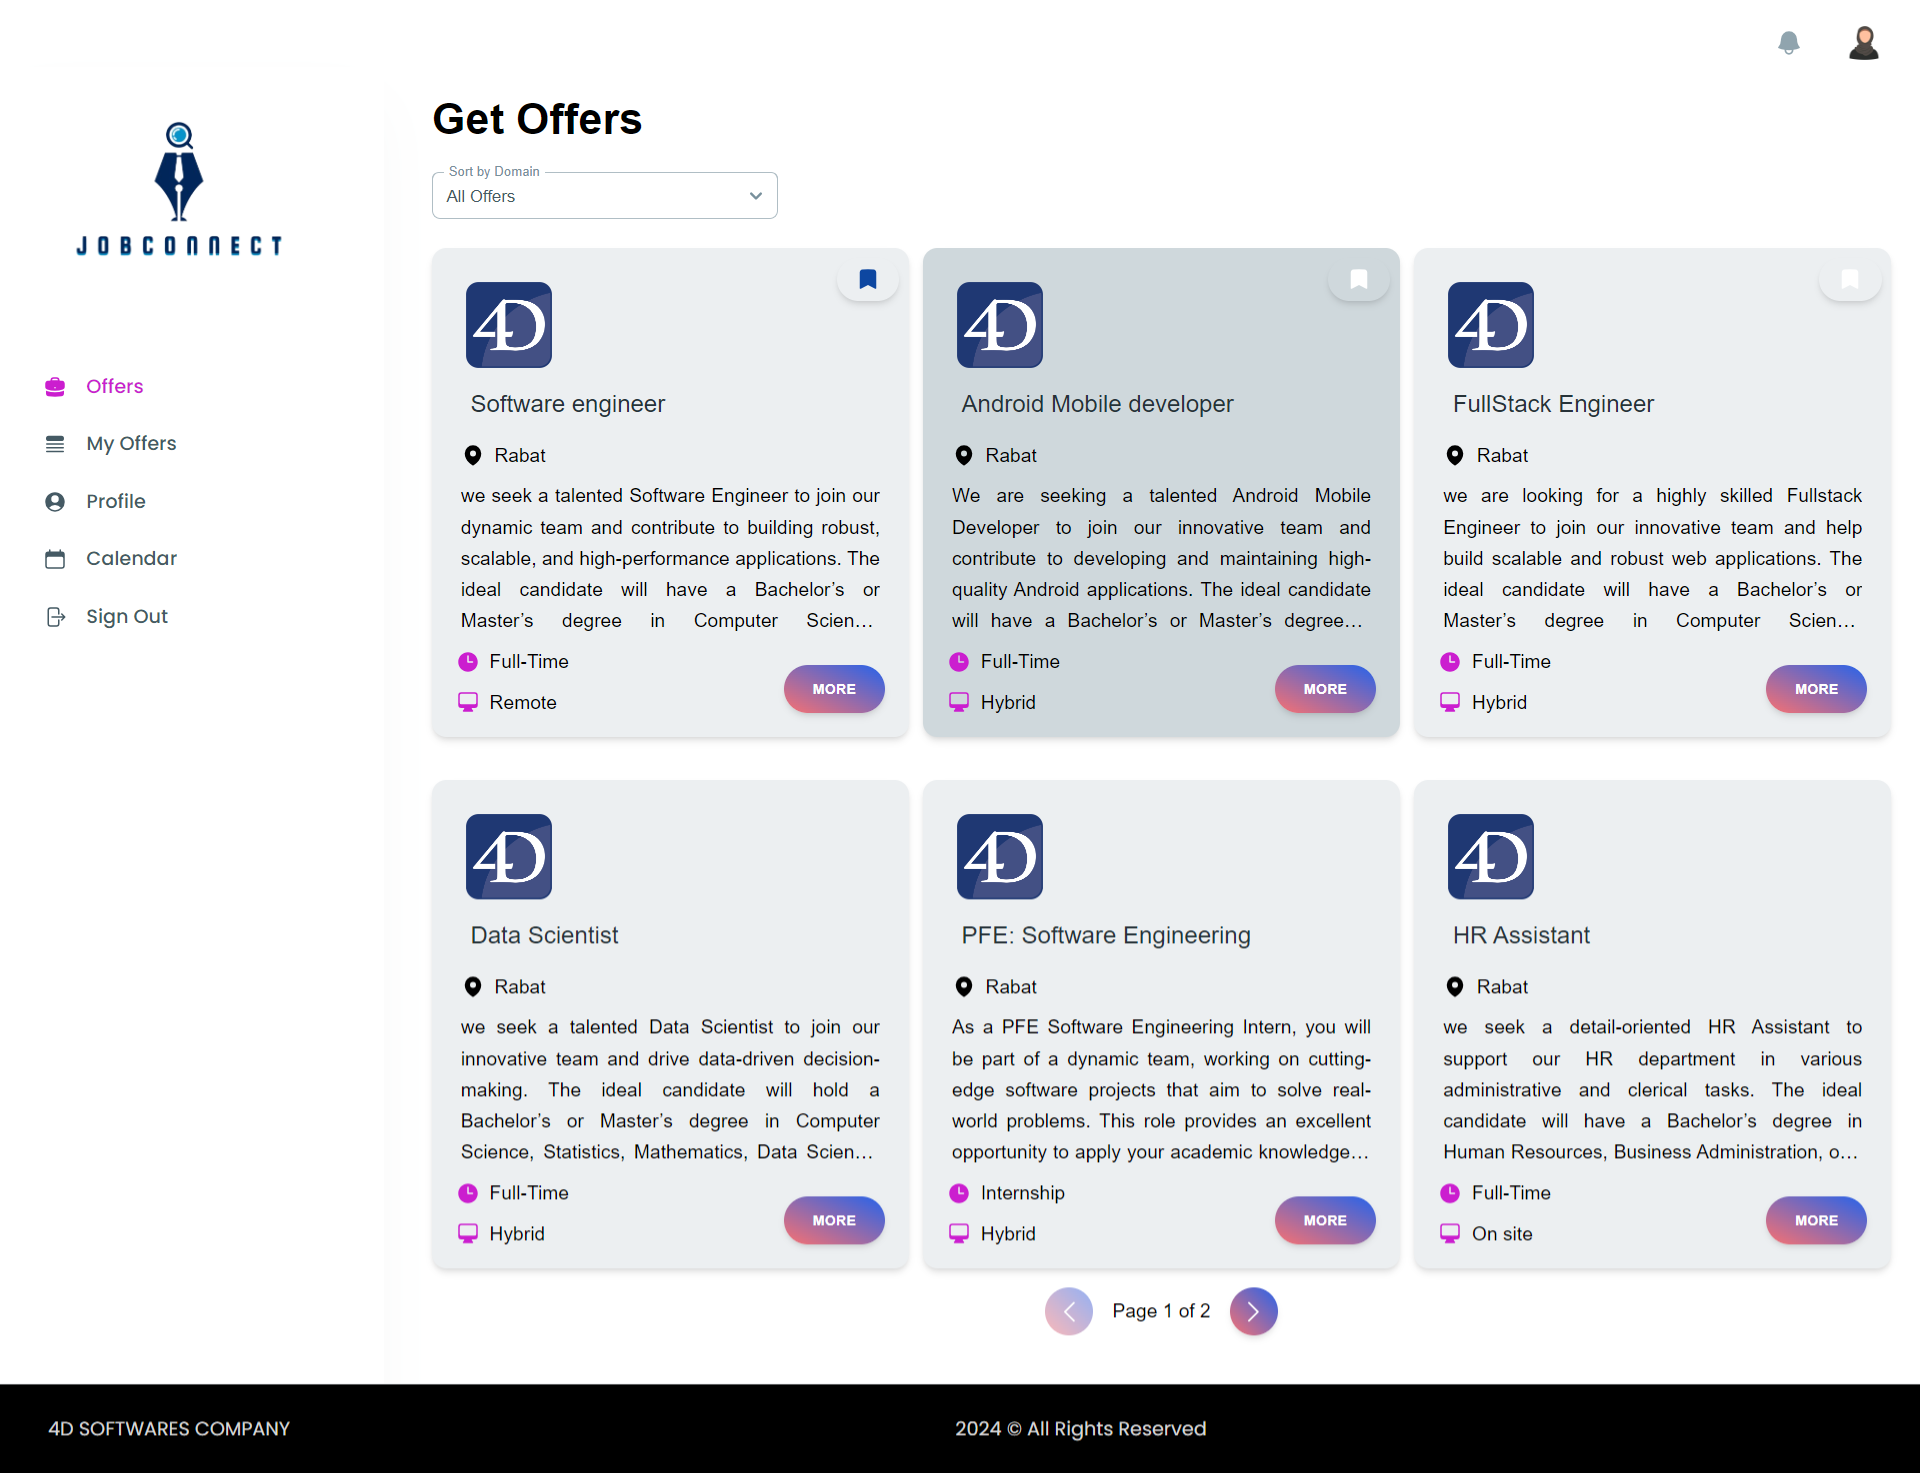
\includegraphics[scale=0.2]{screens/cartes.png} 
   \caption{Liste des offres}
   \label{fig:listOffers}
\end{figure}

Comme illustré dans la figure \ref{fig:detailsOffre}, chaque 
carte est dotée de deux boutons. Le premier, intitulé "More", 
permet au candidat d'accéder à une page détaillant l'offre. 
Le deuxième est pour enregistrer l'offre afin de lui accéder par la suite.
Sur cette page, sont présentés aussi le  titre  de  l'offre,  
sa  localisation,  son mode de travail, le type de contrat, 
la description du  poste,  ainsi  que  les exigences 
spécifiques du poste.
\newline
\begin{figure}[htb]
   \centering
   \includegraphics[scale=0.2]{screens/consultOffer.png} 
   \caption{Consulter le detail d'une offre}
   \label{fig:detailsOffre}
\end{figure}
\vspace{3cm}

Si le candidat souhaite postuler à l'offre, il peut cliquer 
sur le  bouton "APPLY NOW". Cela affichera une boîte de 
dialogue confirmant la candidature à l'offre, comme illustré
dans la figure \ref{fig:detailsOffre}.
\newline

\begin{figure}[htbp]
   \centering
   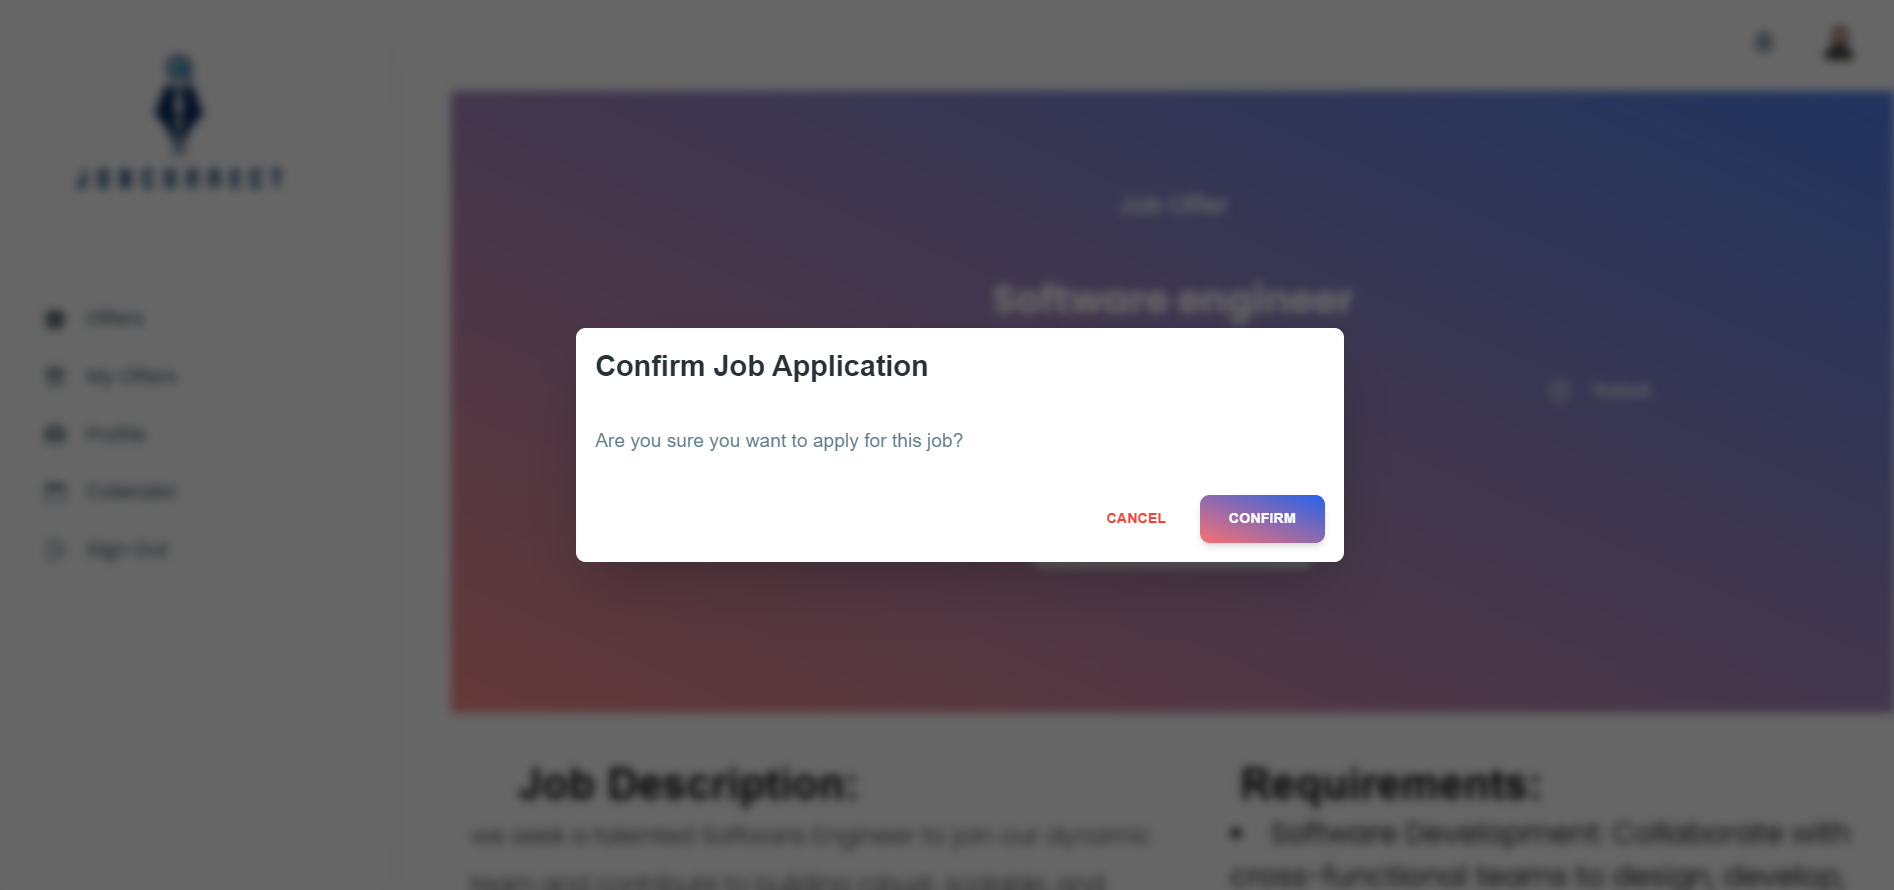
\includegraphics[scale=0.2]{screens/confirmJob2.png} 
   \caption{Confirmation de candidature}
   \label{fig:listOffers}
\end{figure}


En postulant à l'offre choisie, un calcul de score de CV s'effectue. 
Si le score du CV dépasse le seuil défini, le candidat devient éligible à passer 
le test et reçoit un email d'invitation illustré dans la figure \ref{fig:inviteTest}. Dans le cas contraire, le candidat n'est 
pas éligible au test.
\vspace{5cm}
\begin{figure}[htbp]
   \centering
   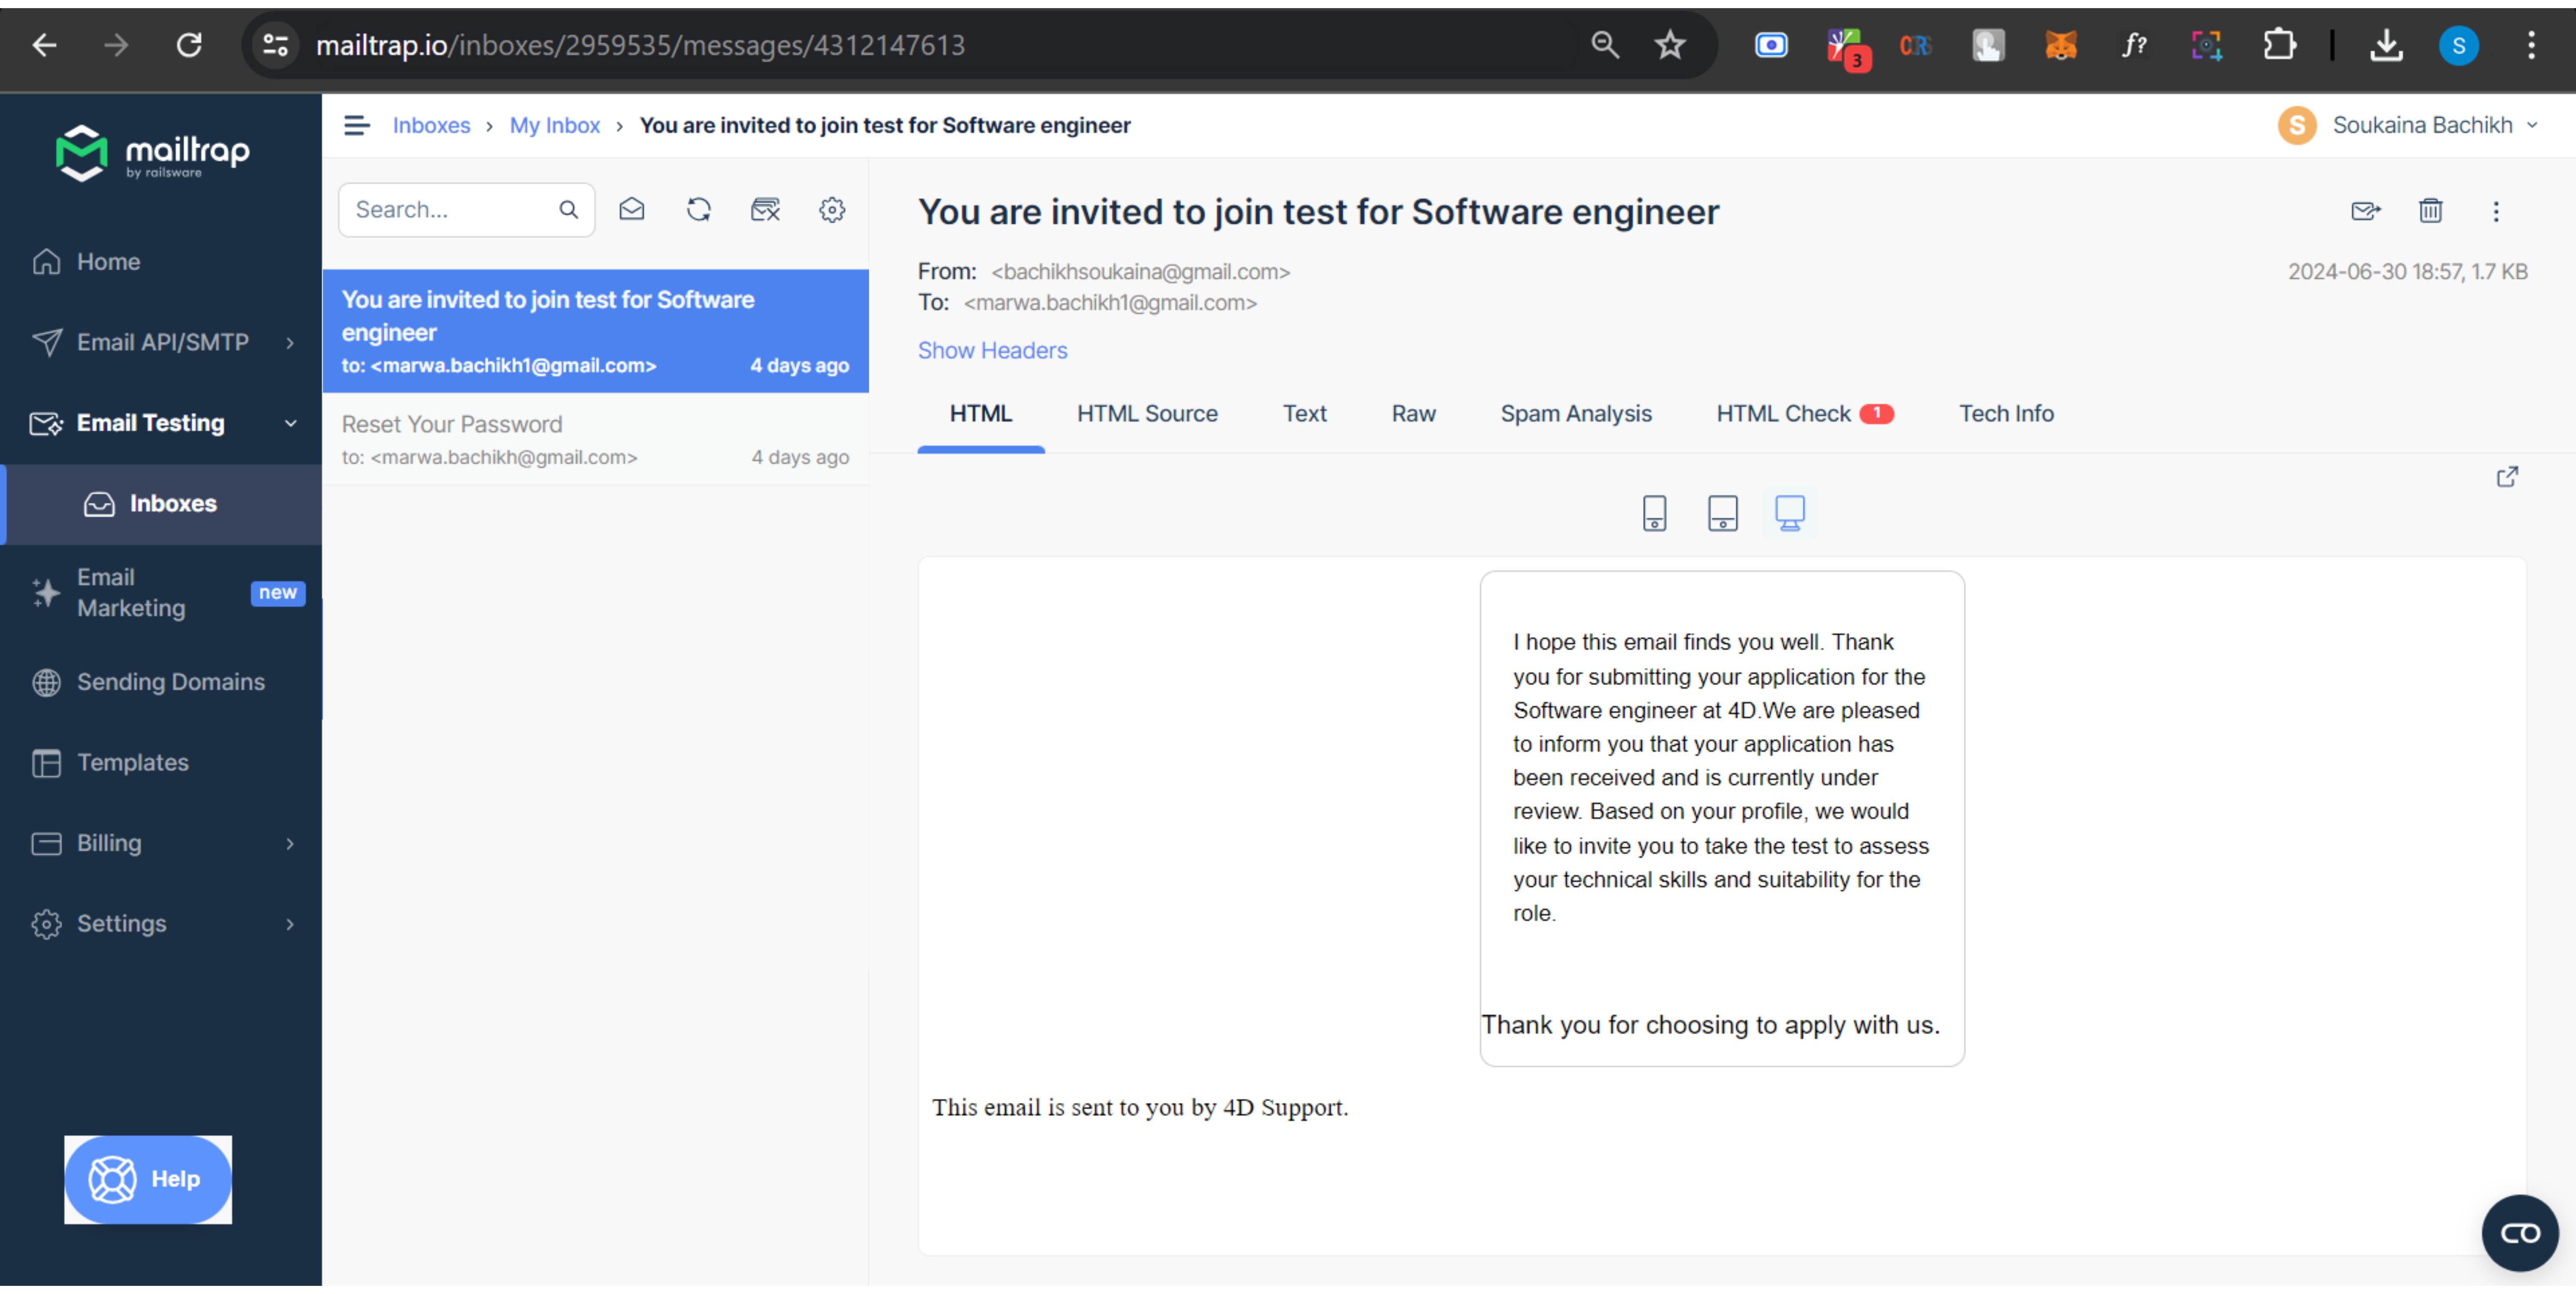
\includegraphics[scale=0.25]{screens/testInvitation.png} 
   \caption{Exemple d'une invitation au test}
   \label{fig:inviteTest}
\end{figure}

\subsubsection{Mes offres}
En cliquant sur le bouton "My offers" situé dans 
le  menu de  gauche, le candidat peut visualiser ses candidatures et les offres qu'il a enregistré. \\
Les offres enregistrés sont disposées sous forme de cartes dans l'onglet "Saved" comme indiqué dans la figure \ref{fig:saved}.
\\

\begin{figure}[htbp]
   \centering
   
\includegraphics[scale=0.2]{screens/saved.png} 
   \caption{Offres enregistrés}
   \label{fig:saved}
\end{figure}

Pour la partie d'historique de candidatures, les  offres auxquelles le  candidat a 
postulé sont affichées dans un tableau en accédant à l'onglet "Applied". Le tableau inclut les éléments suivants: le titre du poste, la date de  
soumission à l'offre, le  lieu, le  statut de la candidature ainsi qu'un bouton "Start test".  
\vspace{3cm}
\begin{figure}[htbp]
   \centering
   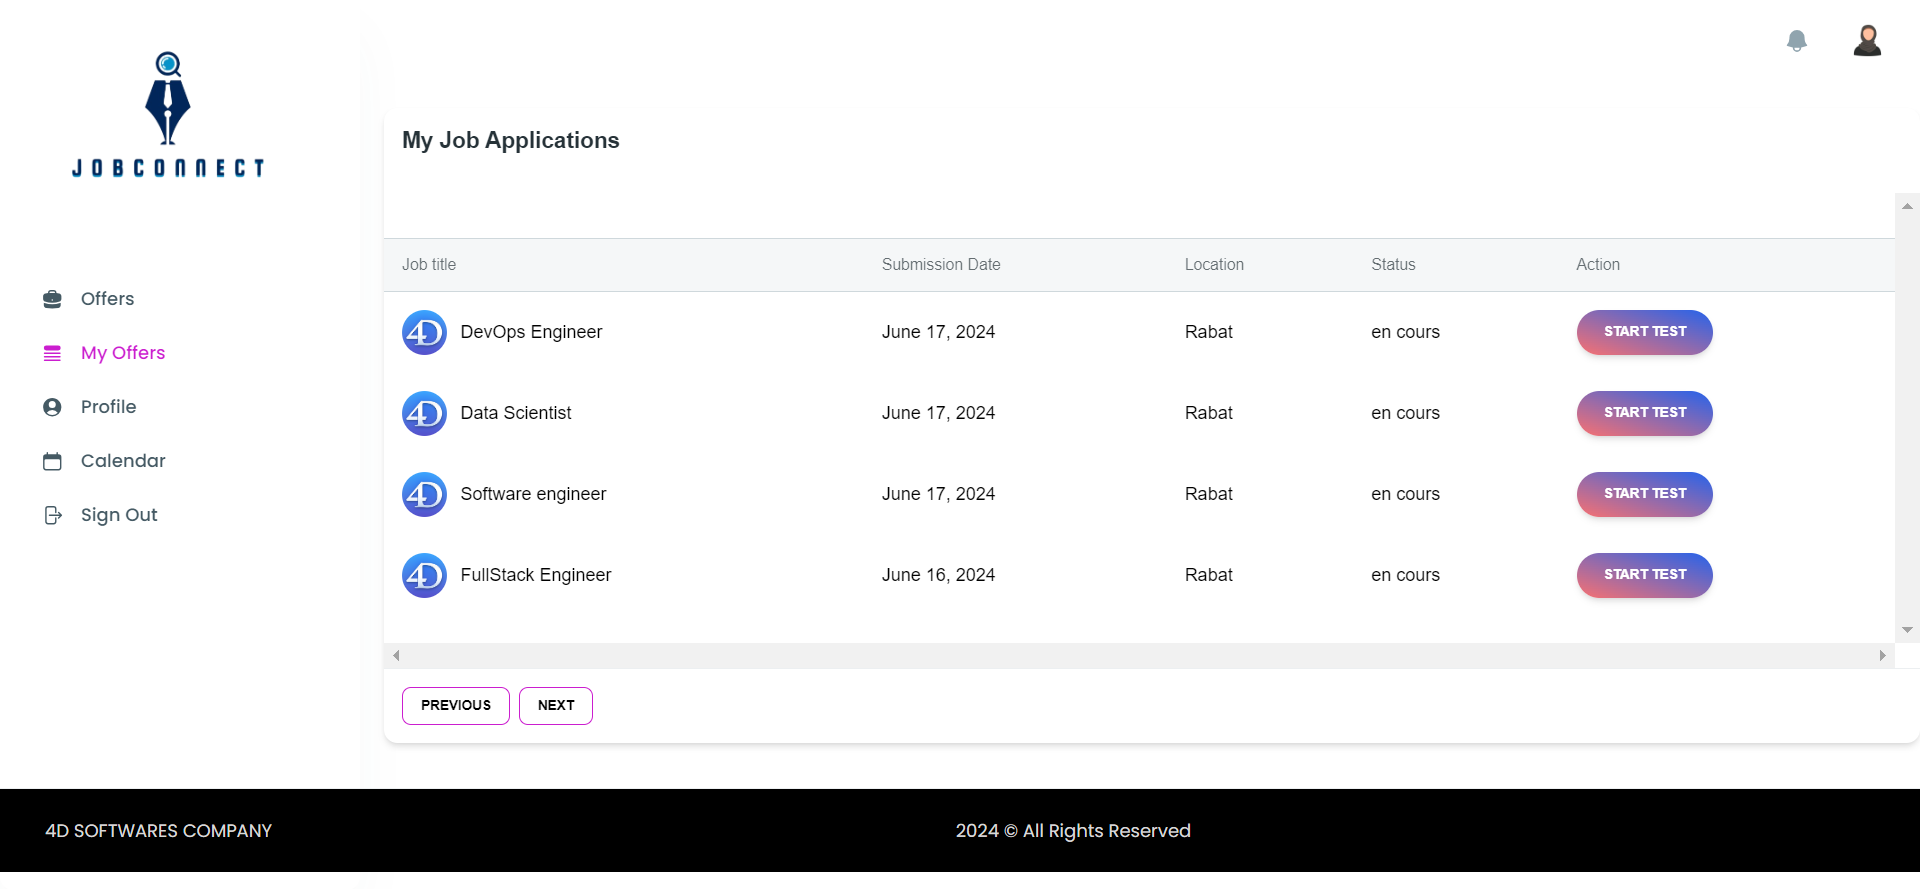
\includegraphics[scale=0.2]{screens/myofffers.png} 
   \caption{Historique de candidatures}
   \label{fig:candidatures}
\end{figure}




\subsubsection{Passer le test}
% Après avoir valider la phase du séléction par cv, le candidat doit passer un test lié à sa candidature.
%  Le test consiste en une série de questions à choix multiples.
%  Ces questions sont générées aléatoirement à partir d'un backlog contenant plusieurs questions en fonction du domaine de l'offre.
%  Cette approche garantit la fiabilité et l'équité des tests  entre les candidats.
%  Les tests ont des limites de temps et un candidat a le droit de passer le test lié à une candidature qu'une seule fois

Après avoir validé la phase de sélection par CV, le candidat doit passer un test. Ce test consiste 
en 
une série de questions à choix multiples générées aléatoirement à partir d'un backlog 
contenant plusieurs questions, adaptées au domaine de l'offre. Cette approche garantit 
une sorte de fiabilité et équité des tests entre les candidats. De plus, chaque test 
a une limite de temps et le candidat n'a droit qu'à une seule tentative par candidature.
\begin{figure}[htbp]
   \centering
   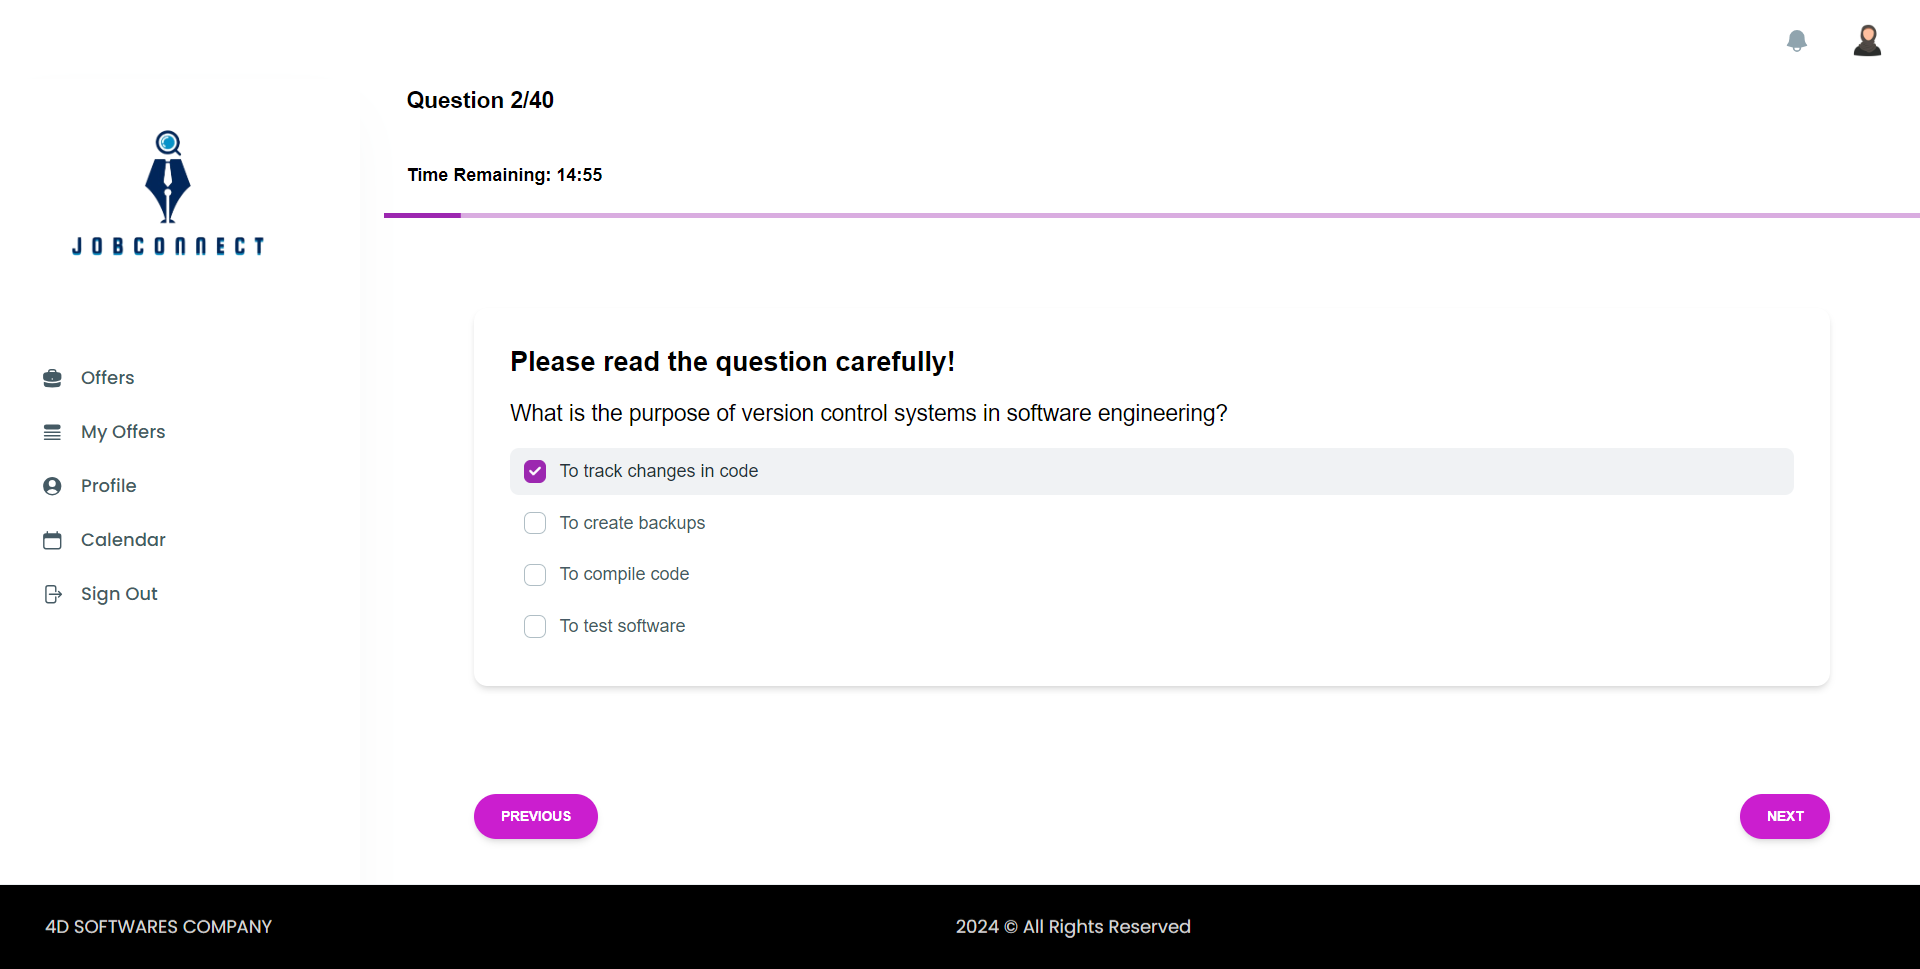
\includegraphics[scale=0.2]{screens/test.png} 
   \caption{Page de test}
   \label{fig:listOffers}
\end{figure}


Si le candidat réussit encore son test, il sera convoqué via email pour passer un entretien avec le recruteur 
chargé de l'offre. Voici un exemple de mail reçu par le candidat représenté dans la figure \ref{fig:mailEntretien}
\vspace{3cm}
\begin{figure}[htbp]
   \centering
   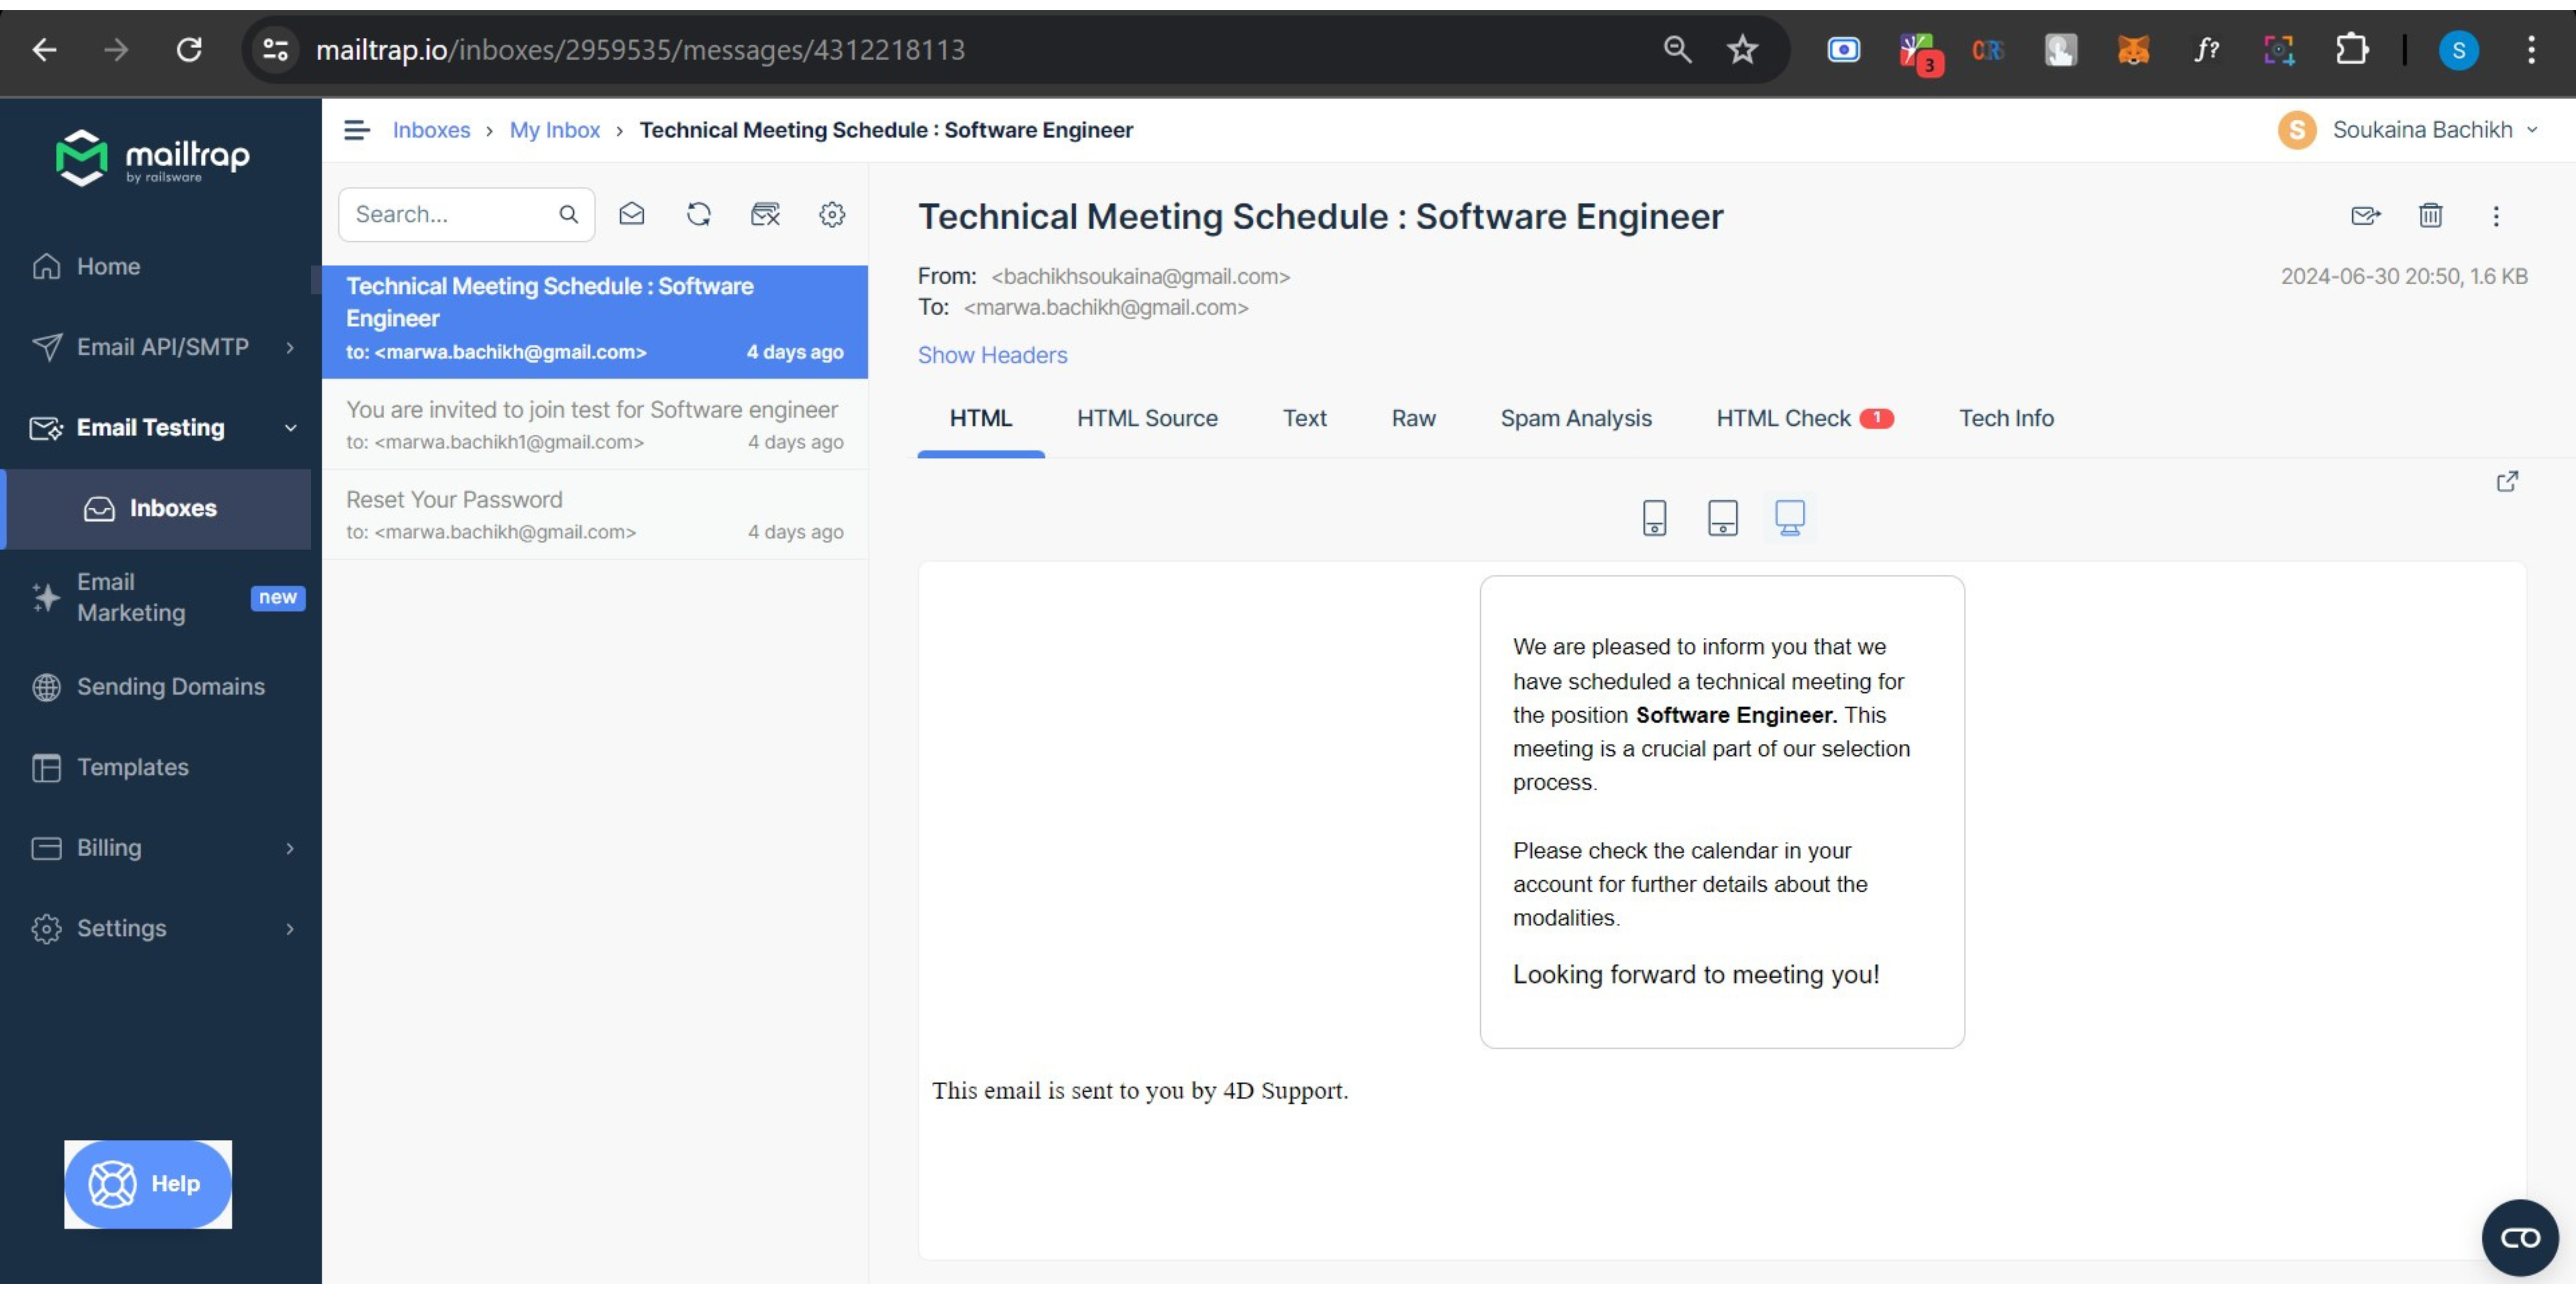
\includegraphics[scale=0.2]{Images/interviewMail.png} 
   \caption{Exemple de convocation à l'entretien}
   \label{fig:mailEntretien}
\end{figure}

\subsubsection{Consulter le calendrier}

Le candidat pourra consulter le calendrier où il trouvera lùense,ble des entretiens qu'il doit passer, comme indiqué dans la figure \ref{fig:calendrierCandid}. 
% Le candidat pourra consulter la page calendrier pour vérifier la 
% date et l'heure de son entretien. Grâce à cette fonctionnalité, les candidats peuvent facilement accéder aux détails de leur rendez-vous, ce qui leur permet de s'organiser efficacement et de se préparer en conséquence pour leur entretien avec le recruteur.
\begin{figure}[htbp]
   \centering
   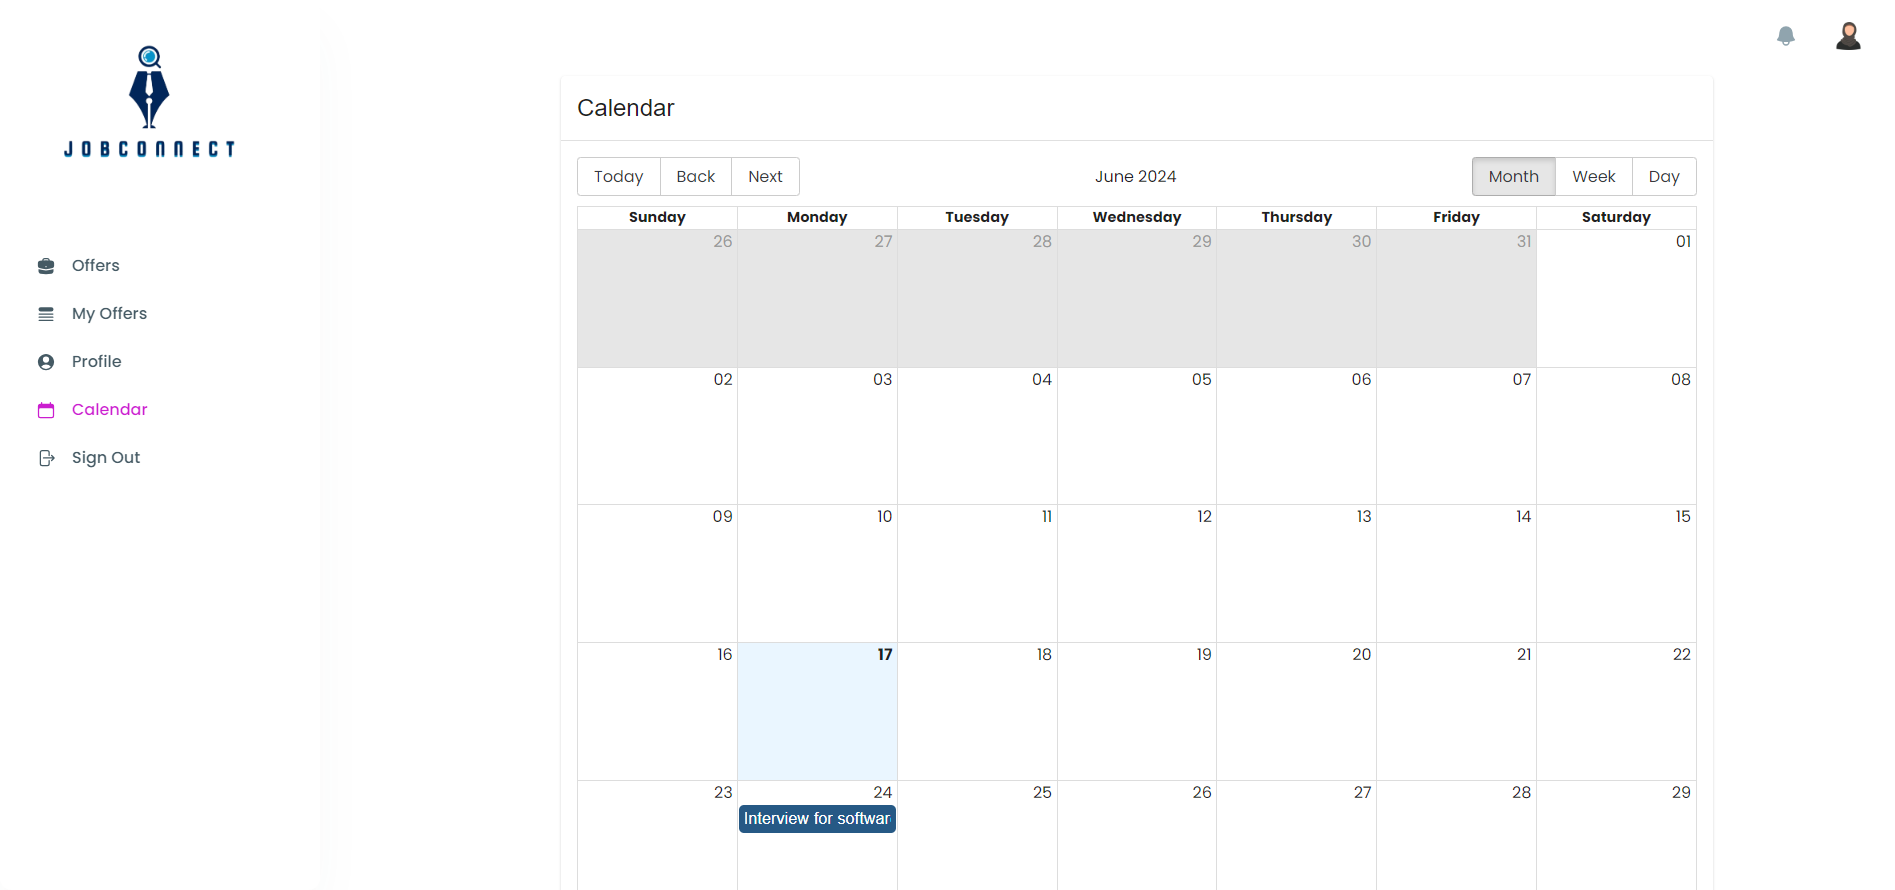
\includegraphics[scale=0.18]{screens/calendarCand.png} 
   \caption{Page de calendrier}
   \label{fig:calendrierCandid}
\end{figure}


% En cliquant sur le titre d'un entretien, il accédera à un dialogue contenant plus de détails tels que la date, l'heure exacte, 
% et l'emplacement de l'entretien. Pour les entretiens présentiel, l'emplacement physique sera précisé, tandis que pour les entretiens en ligne, un lien vers Zoom ou toute autre plateforme similaire sera fourni.
En cliquant sur le titre d'un entretien, le candidat accédera à un dialogue contenant plus de détails, tels que la date, l'heure exacte 
et l'emplacement de l'entretien. Pour les entretiens en présentiel, l'emplacement physique sera précisé, tandis que pour les entretiens en ligne, 
un lien vers Zoom ou toute autre plateforme similaire sera fourni.
% \vspace{2cm}
\begin{figure}[htbp]
   \centering
   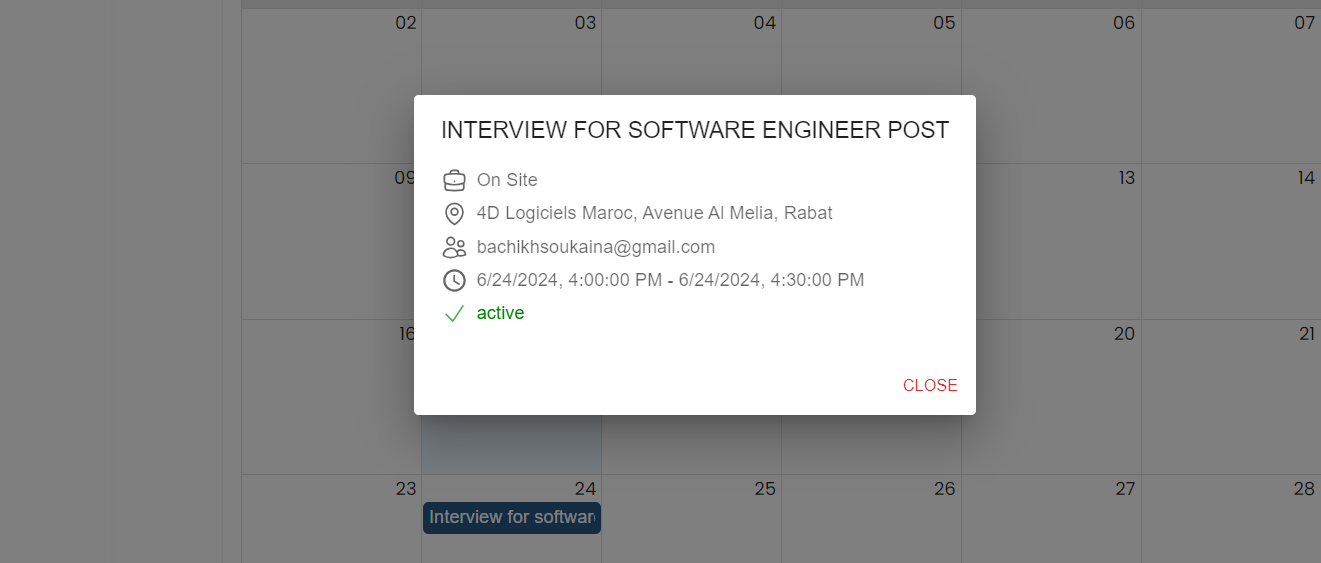
\includegraphics[scale=0.3]{screens/detail interview.png} 
   \caption{Détails de l'entretien}
   \label{fig:listOffers}
\end{figure}

% don't forget to uncomment
\subsection{Espace recruteur}
\subsubsection{Page d'accueil du recruteur}
Cette section est dédiée aux recruteurs, qui doivent s'authentifier pour accéder 
directement à leur page d'accueil, illustrée dans la figure\ref{fig:homeRecr}. La première 
partie de cette page présente les statistiques détaillées des offres publiées 
par le recruteur, organisées par localisation et département. 
% Cette visualisation permet de suivre l'évolution des indicateurs de performance 
% des offres, notamment le nombre total d'offres actives, le nombre de candidatures 
% reçues pour chaque poste, et d'autres métriques pertinentes. 

\begin{figure}[htbp]
   \centering
   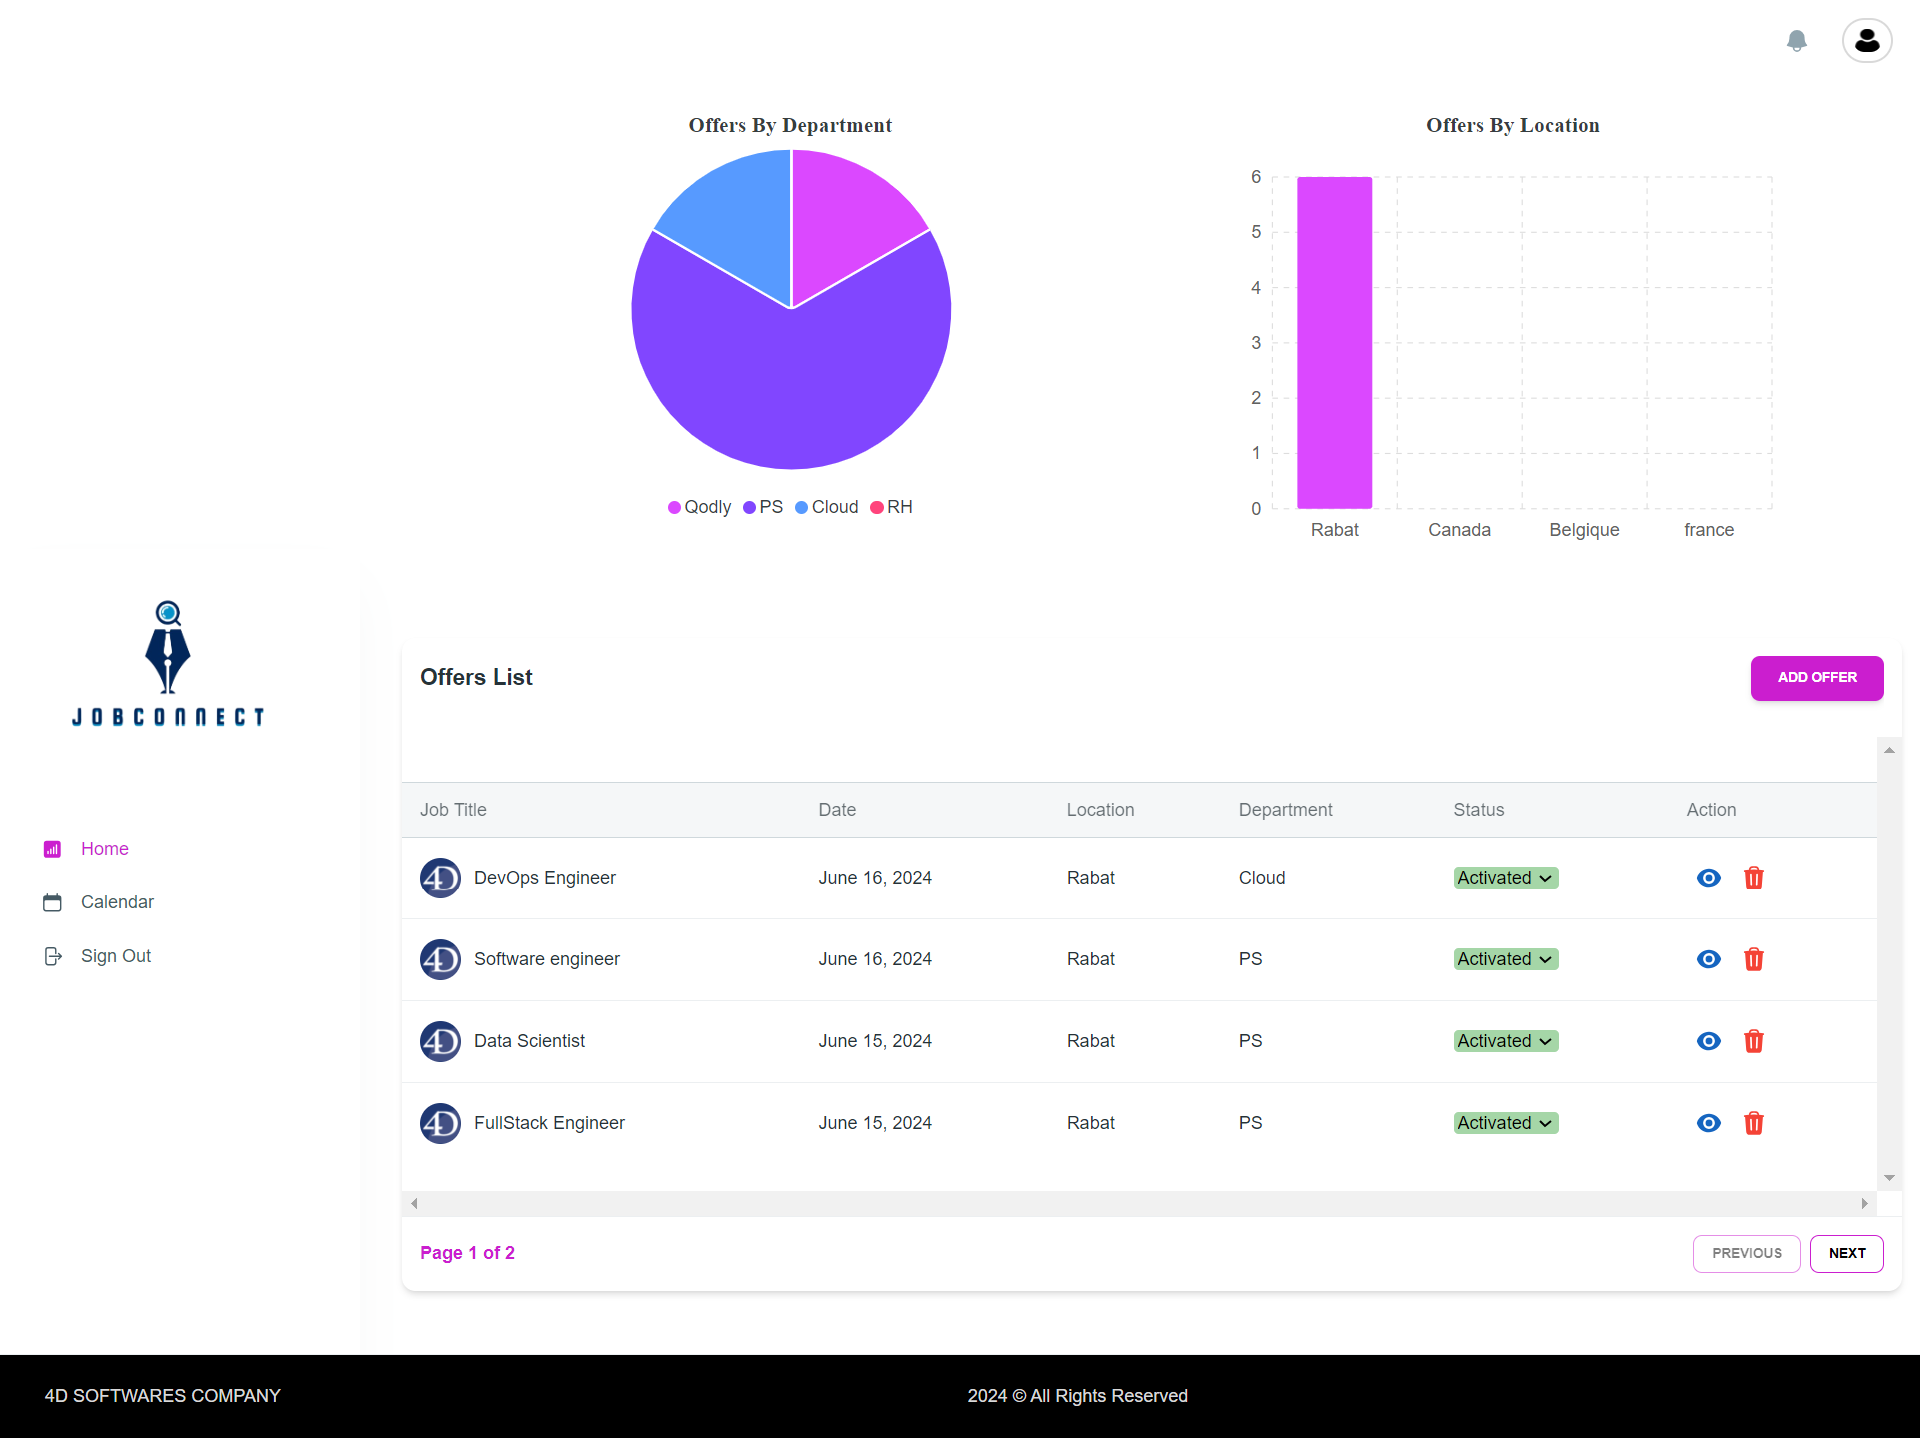
\includegraphics[scale=0.18]{screens/homeRecr.png} 
   \caption{Page d'accueil du recruteur}
   \label{fig:homeRecr}
\end{figure}

La deuxième partie de cette page d'accueil offre une liste détaillée de toutes 
les offres d'emploi actuellement gérées par le recruteur. Chaque offre est 
présentée avec son titre, sa date de publication et son statut (actif ou clos). 
Pour chaque offre, le recruteur a la possibilité de visualiser les détails 
complets. De plus, un bouton "Add Offer" est 
disponible pour permettre aux recruteurs de créer de nouvelles opportunités 
d'emploi en fonction des besoins évolutifs de l'organisme.

\subsubsection{Publier une offre}

Cette fonctionnalité permet aux recruteurs de créer une nouvelle offre, en saisissant les informations suivantes.
\begin{enumerate}
   \item Job Title (Titre du poste)
   \item Job Location (Lieu de travail)
   \item Work Mode (Mode de travail)
   \item Job Type (Type de contrat)
   \item Required Skills (Compétences requises)
   \item Department (Département)
   \item Domain (Domaine)
   \item Requirements (Exigences)
   \item Job Description (Description du poste)
\end{enumerate}

\begin{figure}[htbp]
   \centering
   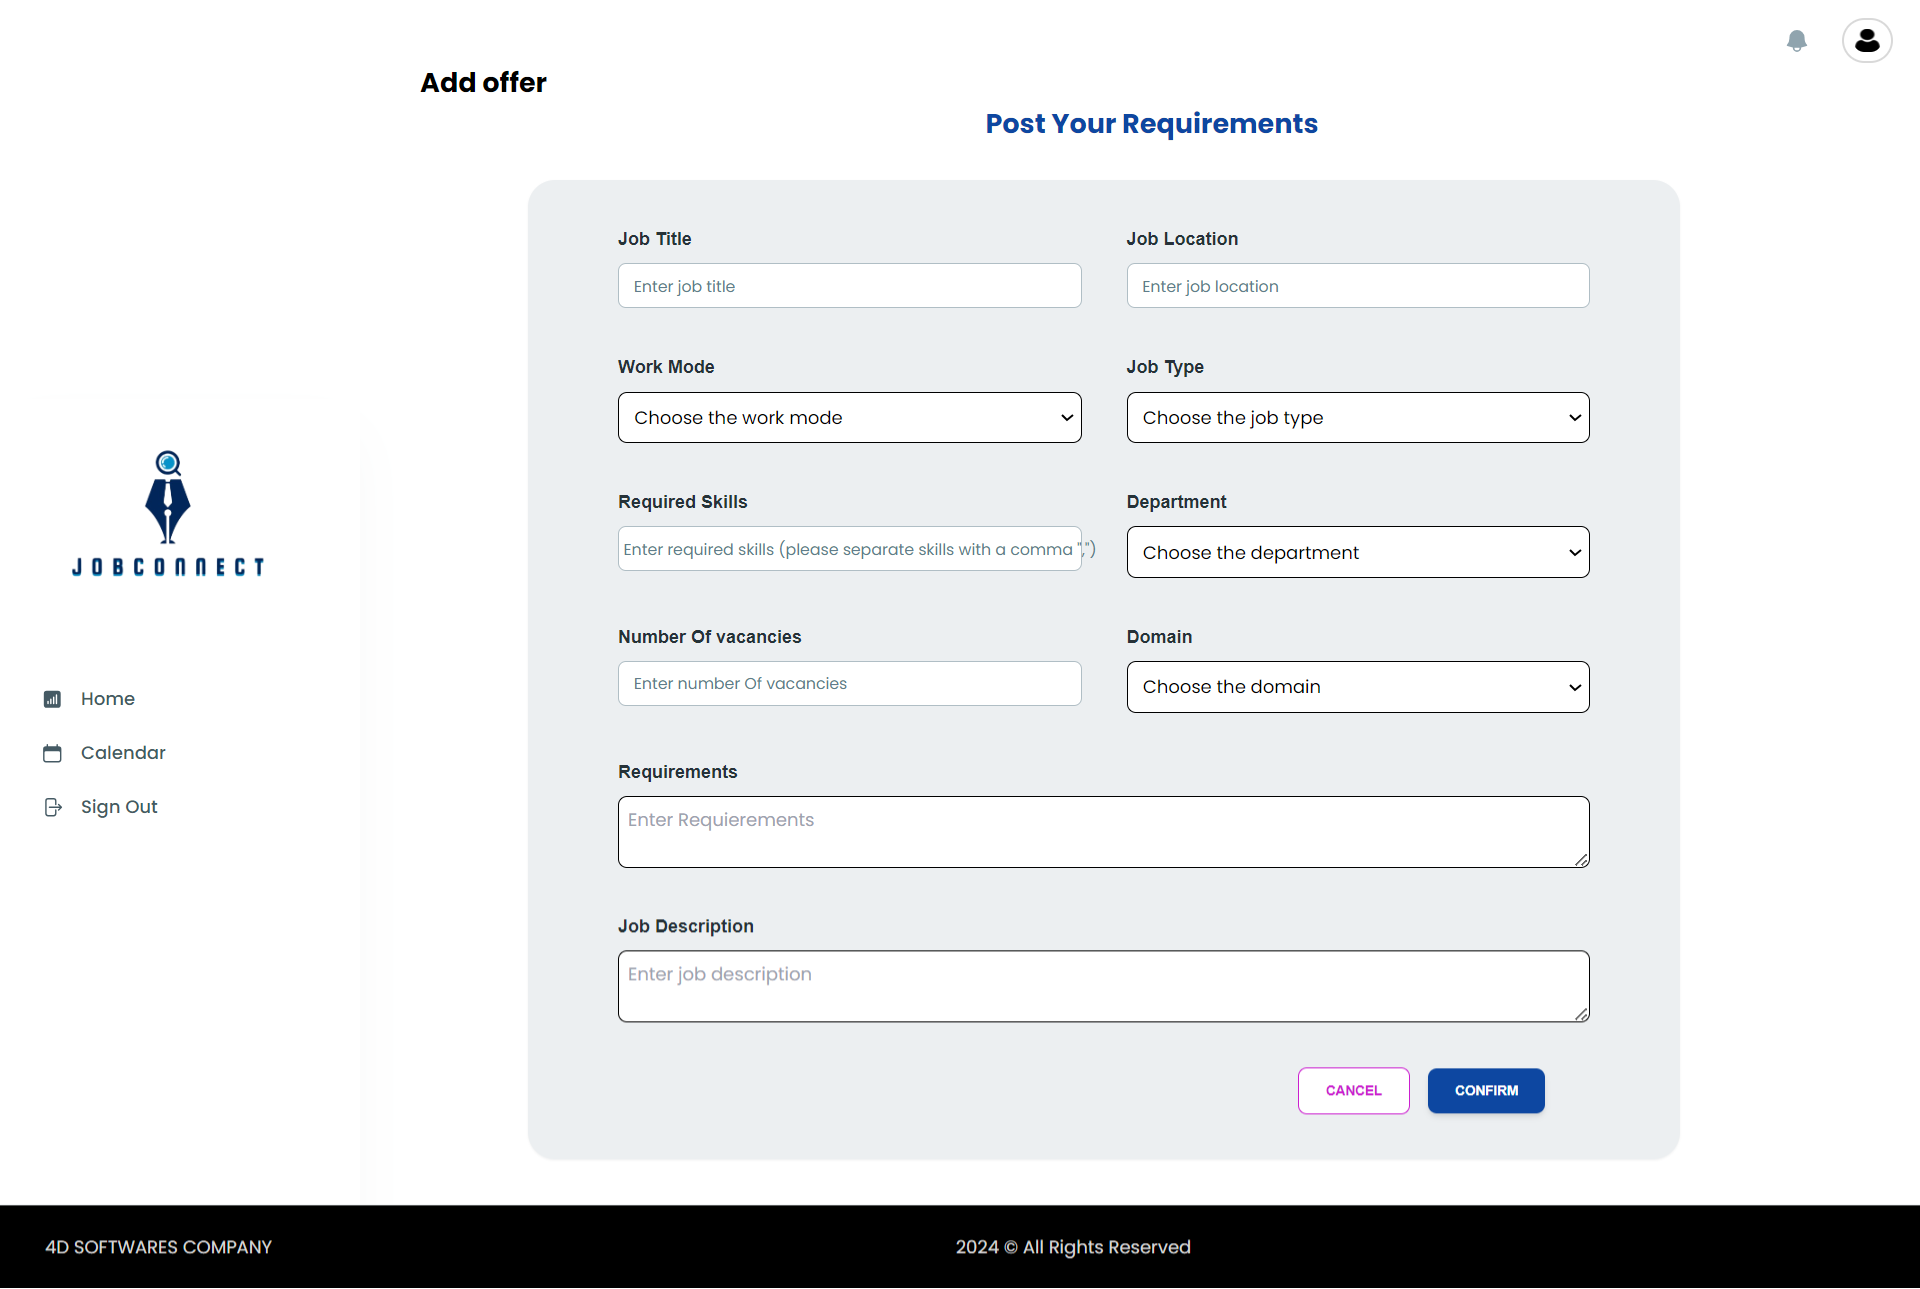
\includegraphics[scale=0.15]{screens/addOffer.png} 
   \caption{Publier une offre d'emploi}
   \label{fig:addOfferFields}
\end{figure}

\subsubsection{Gestion de l'offre d'emploi}
Cette page est essentielle pour le recruteur, lui permettant de gérer en détail chaque offre d'emploi publiée. Elle se compose de plusieurs sections :
\begin{figure}[htbp]
   \centering
   \includegraphics[scale=0.17]{screens/detailsOfferRecr.png}
   \caption{Gestion de l'offre d'emploi}
   \label{fig:listOffers}
\end{figure}

\paragraph{- Informations sur l'offre}
Cette section présente les informations essentielles 
relatives à l'offre d'emploi. Le recruteur peut y voir et 
ainsi modifier les détails en cas de changement des besoins. 

\paragraph*{- Modification de l'offre}
Un bouton "Edit Offer" permet au recruteur de mettre 
à jour les informations de l'offre. 
Cela ouvre un formulaire où il peut ajuster les détails 
de l'offre.
\begin{figure}[htbp]
   \centering
   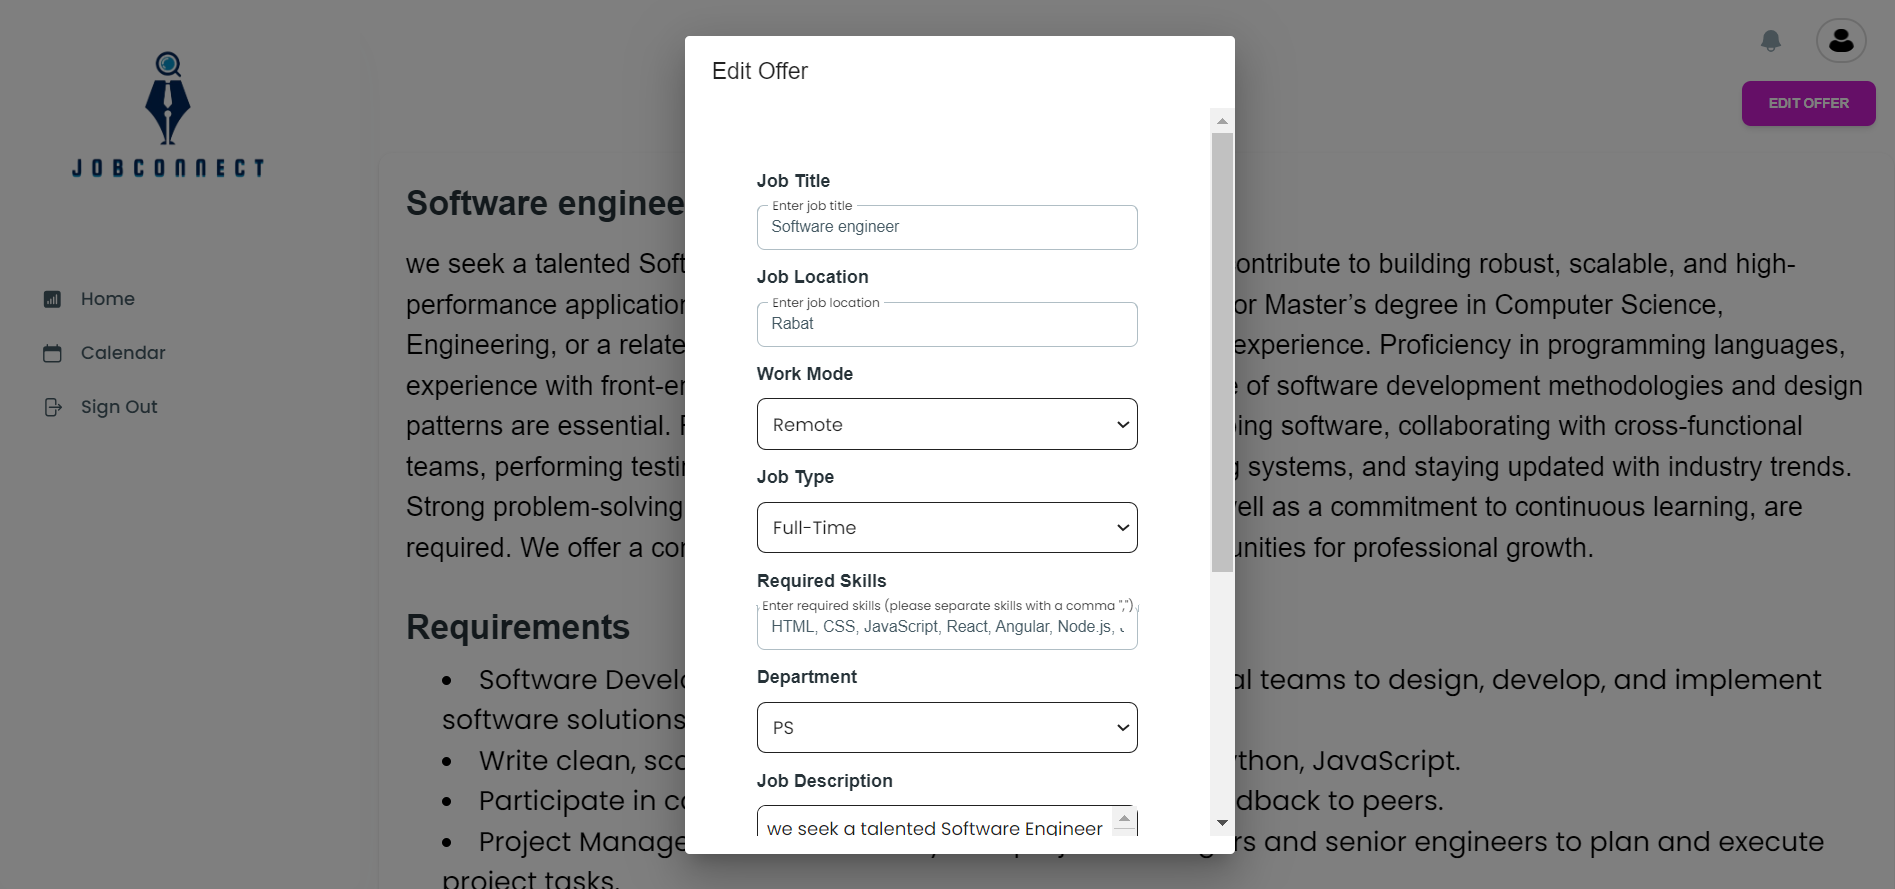
\includegraphics[scale=0.2]{screens/editOffer.png}
   \caption{Modification de l'offre}
   \label{fig
   }
   \end{figure}

\paragraph*{- Liste des candidats}
Cette section permet au recruteur de visualiser et gérer les candidatures pour une offre d'emploi spécifique. 
Chaque entrée de candidature comprend les détails suivants :
\begin{itemize}
   \item[•] Nom du candidat : Le nom complet du candidat
   \item[•] Email : L'adresse email du candidat.
   \item[•] Score du CV : Un score numérique représentant la compatibilité du CV du candidat avec les exigences de l'offre d'emploi.
   \item[•] Résultat du test : Indique si le candidat a réussi le test, et éventuellement, la note obtenue après l'évaluation.
   \item[•] Statut de la candidature : État actuel de la candidature (En cours, Rejetée, Acceptée).
   \item[•] Actions disponibles pour chaque candidature :
      \begin{enumerate}
         \item Voir le CV : Permet aux recruteurs de consulter le CV complet du candidat pour évaluer ses qualifications plus en détail.
         \item Planifier un entretien : Ouvre une interface pour programmer un entretien avec le candidat sélectionné.
         \item Accepter le candidat : Change le statut de la candidature à "Acceptée", indiquant que le candidat a été retenu pour le poste,
         par la suite un mail de confirmation est envoyé au candidat. 
         \newline
         \newline
      \end{enumerate}
\end{itemize}
\vspace{3cm}
\begin{figure}[htbp]
   \centering
   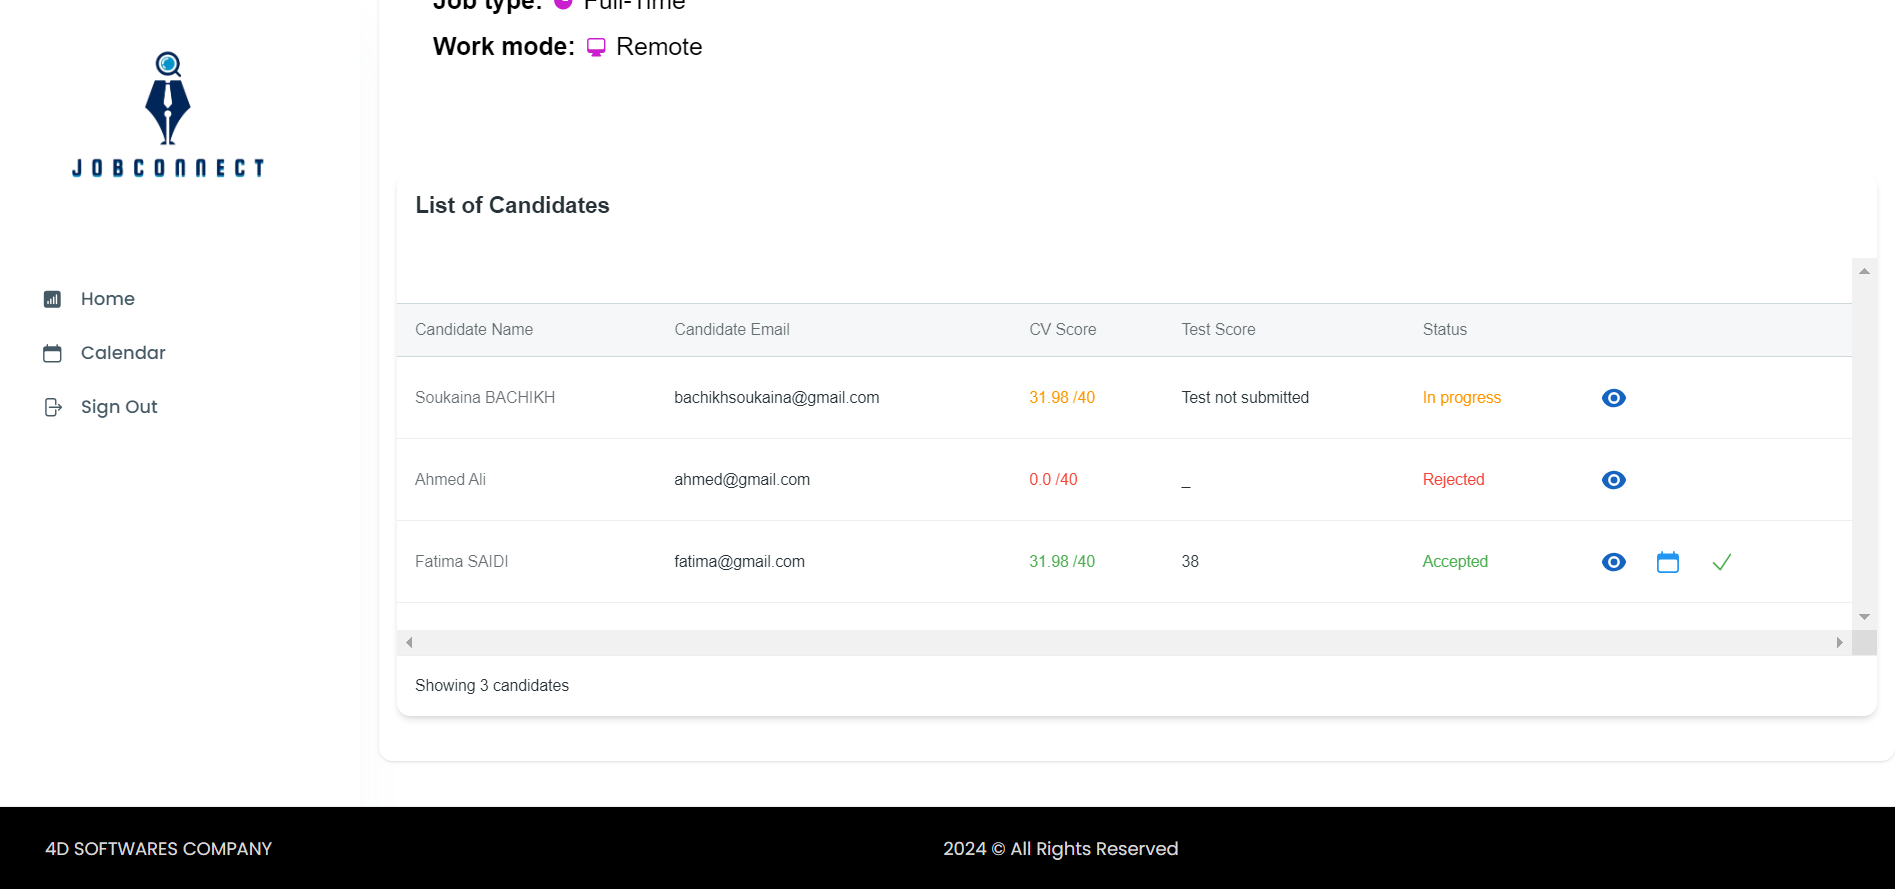
\includegraphics[scale=0.18]{screens/listCandidates.png}
   \caption{Liste des candidats ayant postulé à l'offre}
   \label{fig:candidaturesRec}
\end{figure}

% Voici un exemple de mail envoyé lorsque le recruteur accepte la candidature d'un candidat, figure \ref{fig:}.
% \begin{figure}[htbp]
%    \centering
%    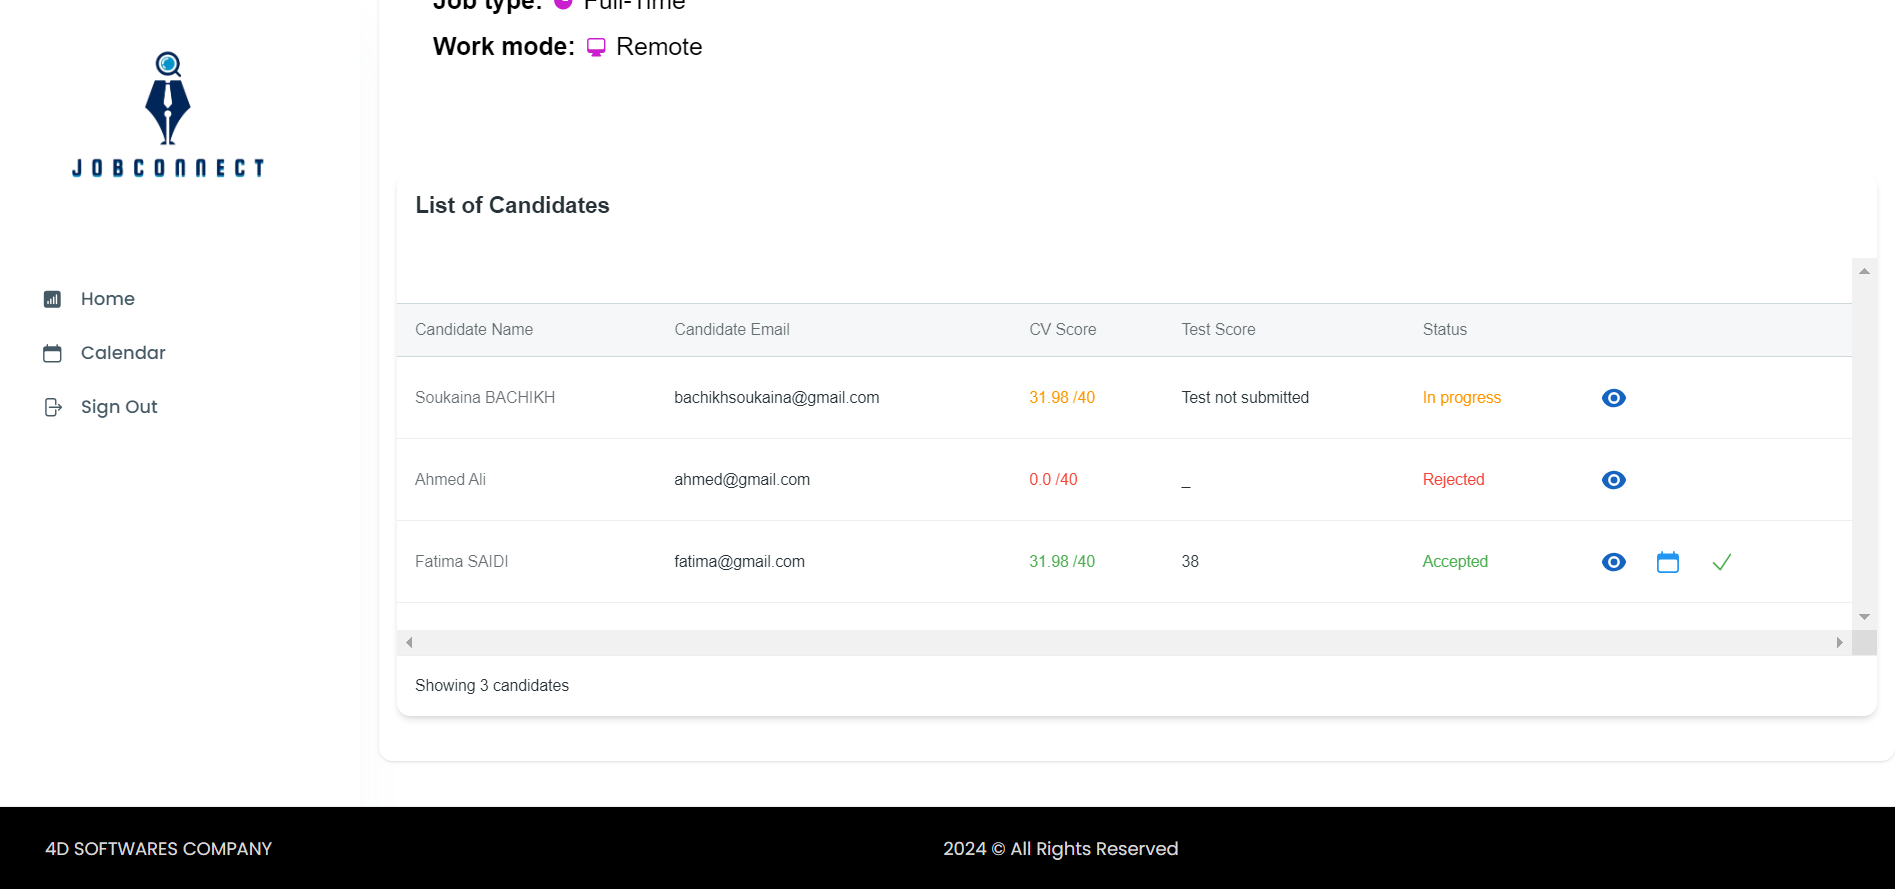
\includegraphics[scale=0.18]{screens/listCandidates.png}
%    \caption{Exemple de mail d'acceptation de candidat}
%    \label{fig:chihaja}
% \end{figure}

\paragraph*{Planifier un entretien}

Après la validation du CV et la réussite du test, le recruteur peut 
planifier un entretien avec le candidat. Cette étape est cruciale pour 
évaluer plus en détail les compétences et l'adéquation du 
candidat avec l'entreprise. 
Le processus est 
réalisé comme suit :

\begin{enumerate}
    \item \textbf{Accès à la planification d'entretien :}
        \begin{itemize}
            \item[•] \textbf{Via l'icône de planification :} En cliquant sur une icône dédiée dans l'interface utilisateur, le recruteur peut accéder à un formulaire de planification d'entretien.
            \item[•] \textbf{Via le menu de gauche :} En naviguant dans le menu de gauche, le recruteur peut accéder directement au calendrier où il peut voir les créneaux disponibles pour planifier l'entretien.
        \end{itemize}
    
    \item \textbf{Sélection du créneau d'entretien :}
        \begin{itemize}
            \item[•] Une fois dans l'interface de planification, le recruteur peut sélectionner un créneau horaire convenable.
            \item[•] Des détails tels que la date, l'heure et l'emplacement de l'entretien peuvent être spécifiés et confirmés dans ce formulaire.
        \end{itemize}
    
    \item \textbf{Confirmation et envoi de l'invitation :}
        \begin{itemize}
            \item[•] Une fois le créneau sélectionné et les détails finalisés, une invitation à l'entretien est envoyé au candidat par email.
            \item[•] L'invitation contient les informations essentielles comme la date, l'heure, l'emplacement physique ou le lien de la réunion en ligne pour l'entretien.
            \\
            \\
            \\
            \\
         \\
         \\
         \end{itemize}
\end{enumerate}

% Exemple d'icône pour la planification d'entretien
\begin{figure}[htbp]
   \centering
   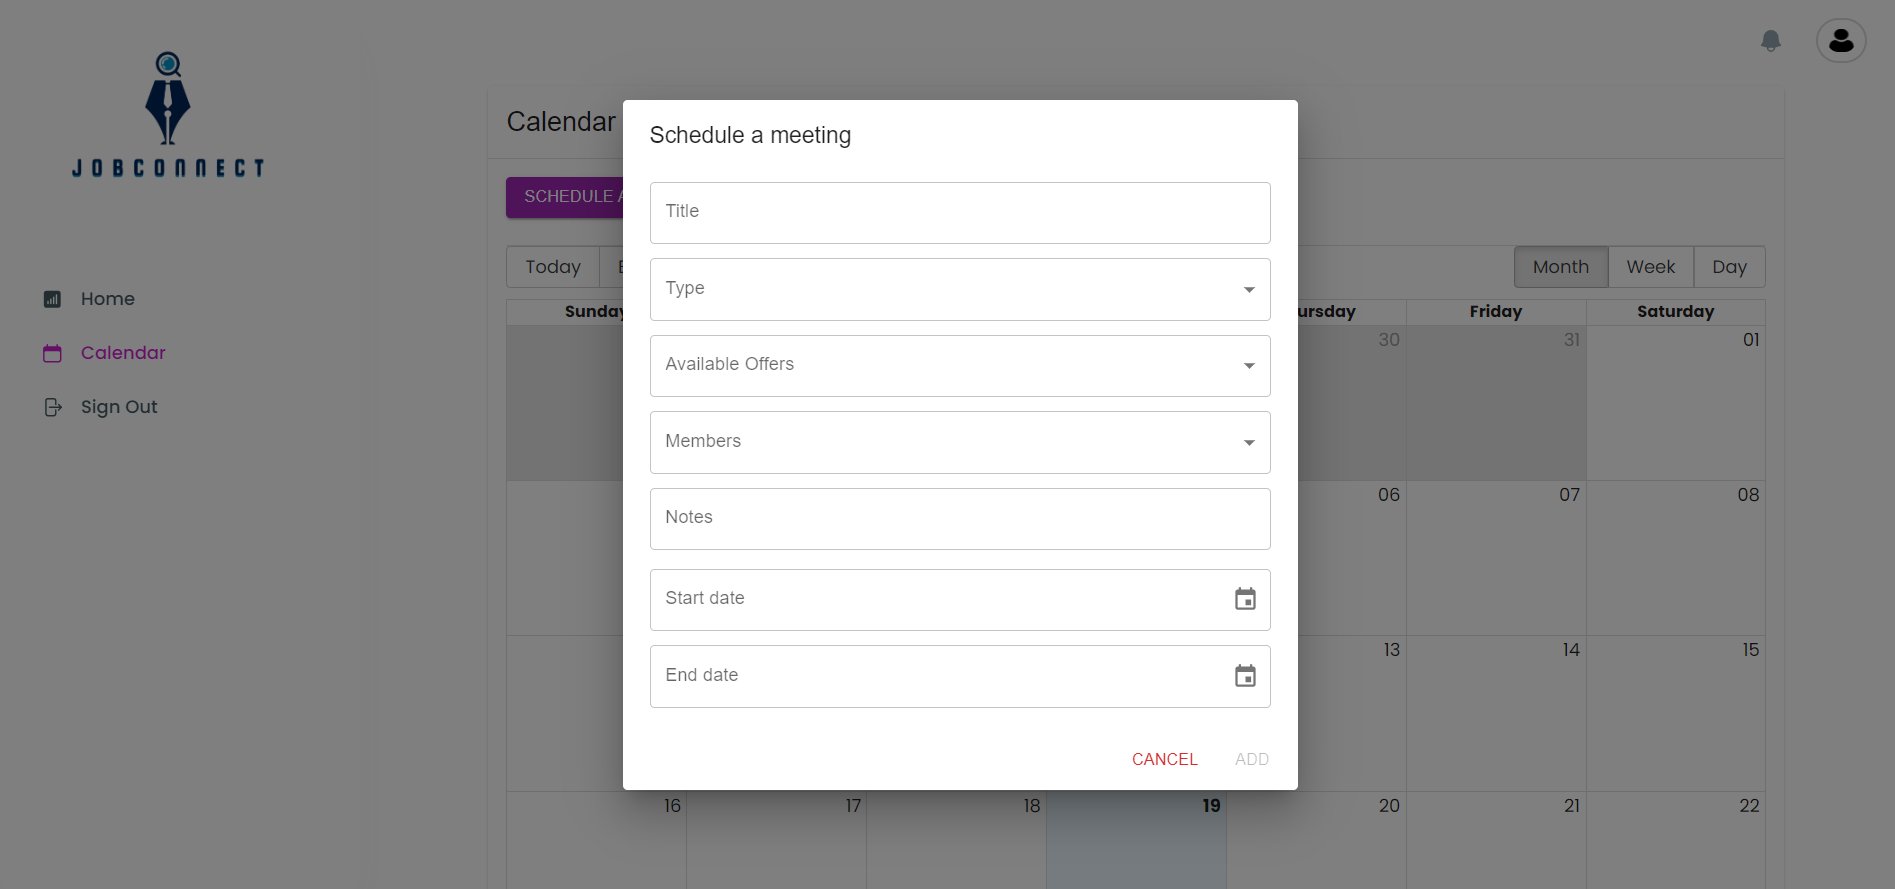
\includegraphics[scale=0.18]{screens/schedule.png} 
   \caption{Planification d'un entretien}
   \label{fig:scheduleIcon}
\end{figure}

\paragraph*{Accepter un candidat}
Une fois que le recruteur a terminé l'entretien avec le candidat,
il pourra accepter le candidat via l'icone de validation dans la figure \ref{fig:candidaturesRec}.
En suite un email est envoyé au candidat pour lui informer de 
l'acceptation de sa candidature, comme illustré dans la figure \ref{fig:mailAccept}.
\begin{figure}[htbp]
   \centering
   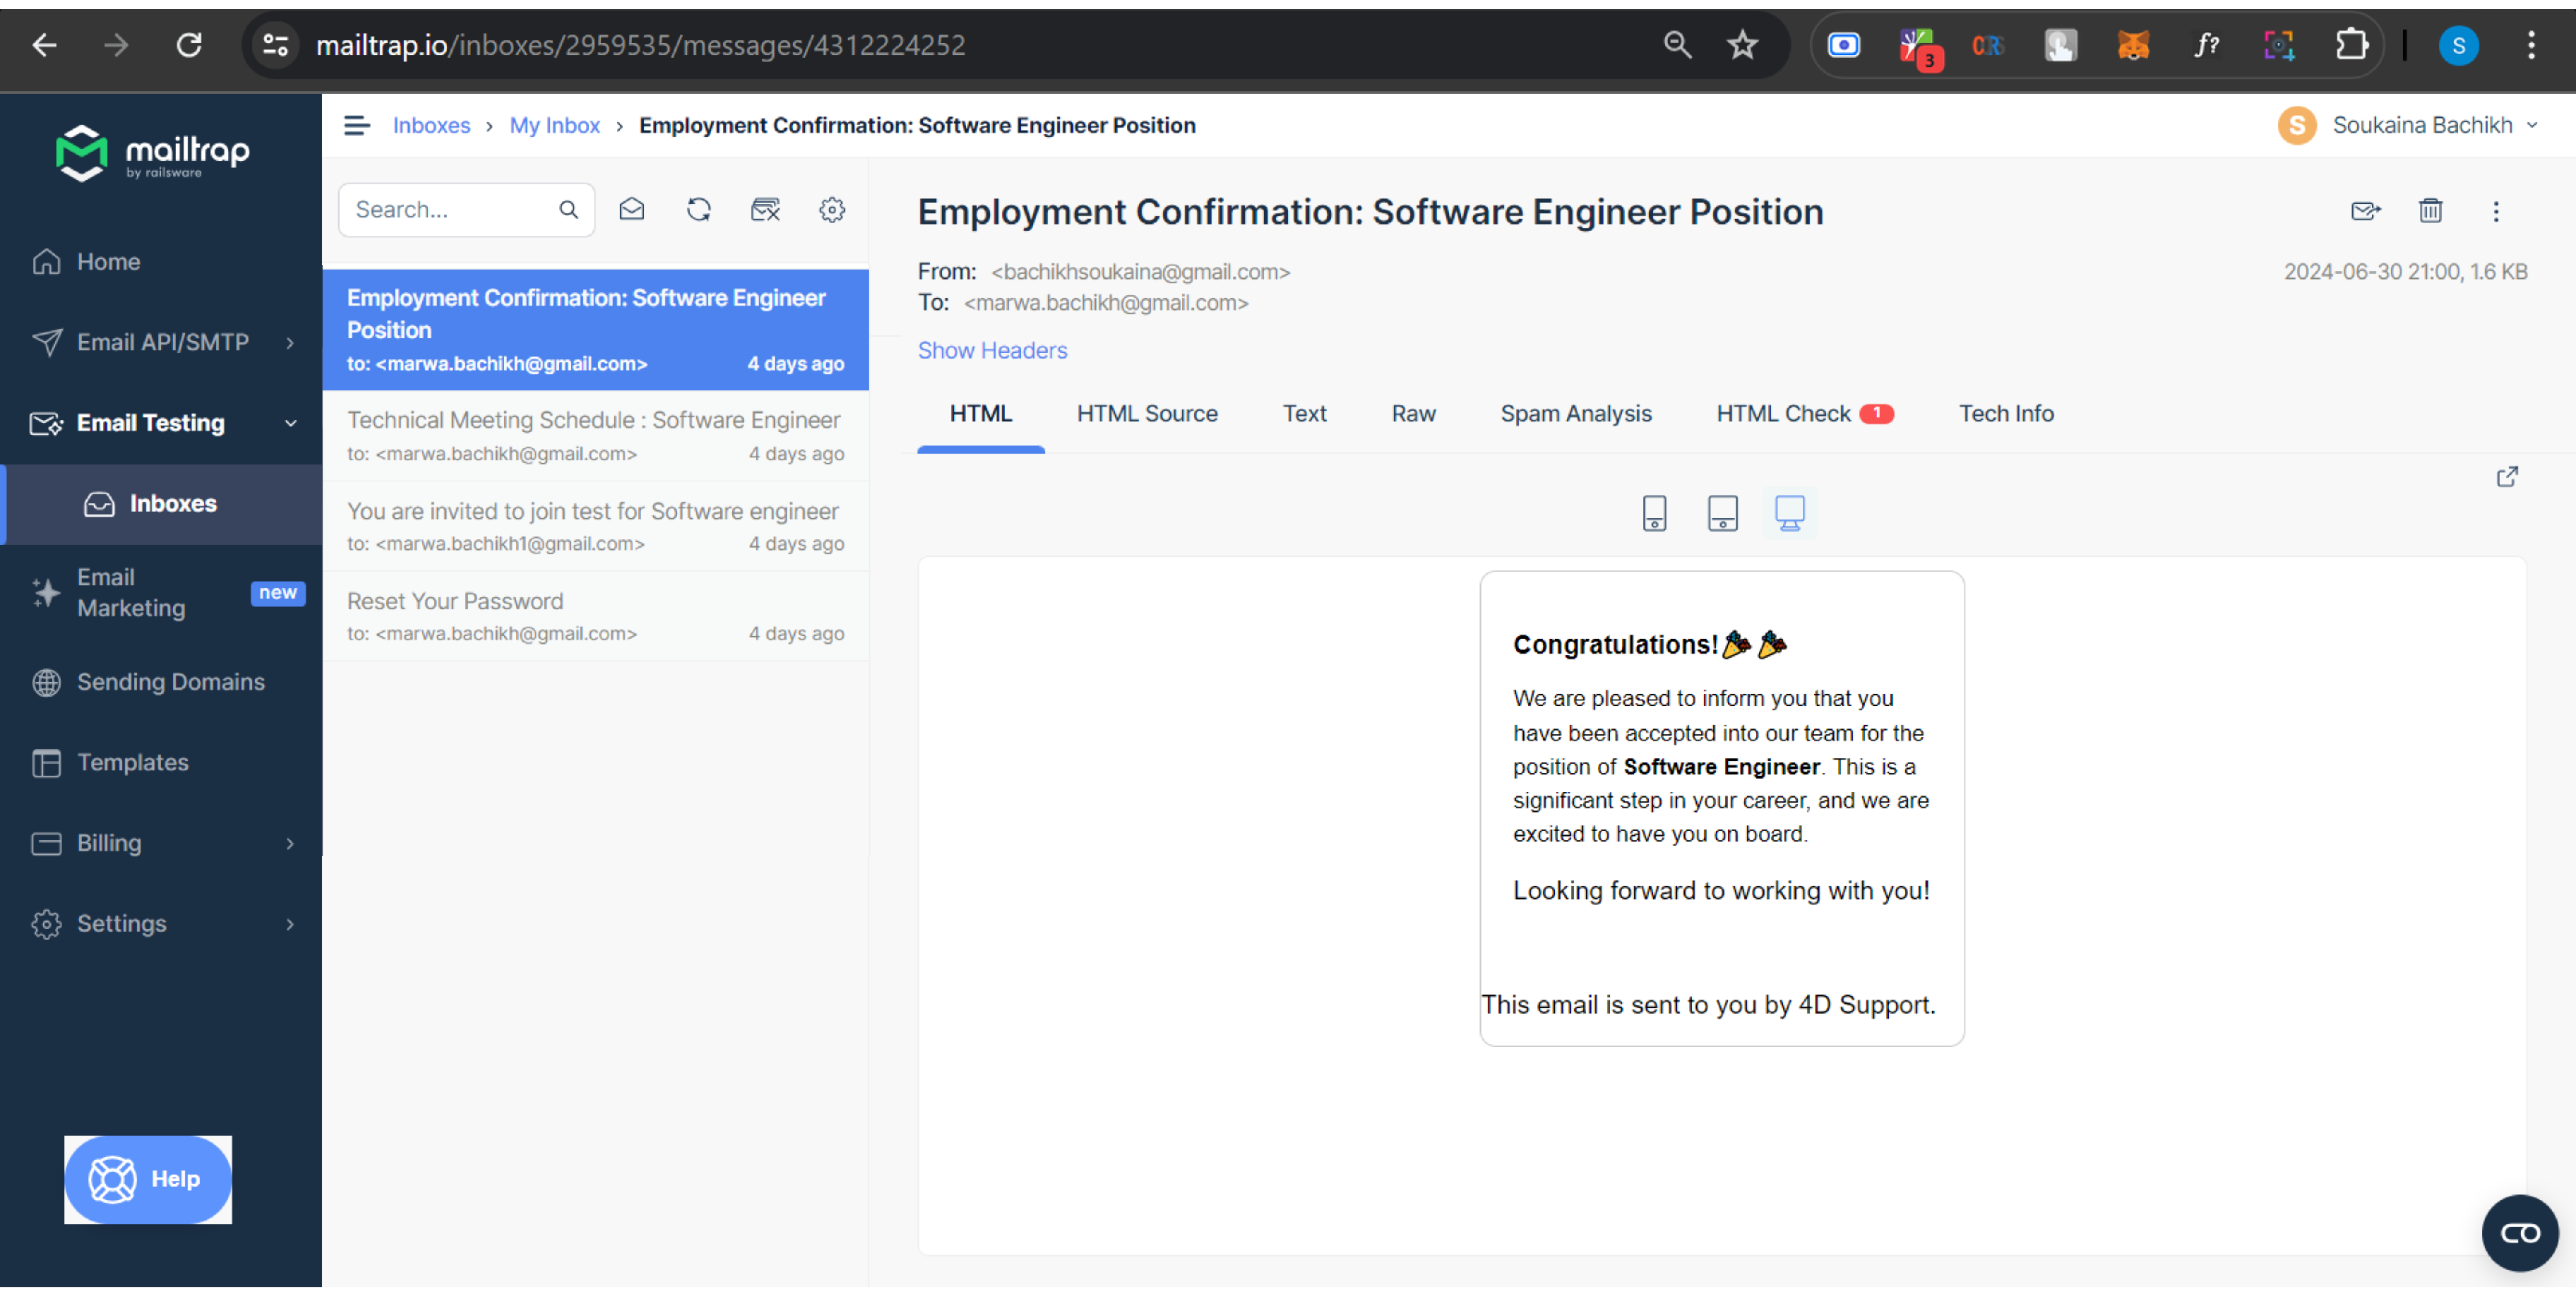
\includegraphics[scale=0.2]{screens/acceptCandidate.png}
   \caption{Accepter un candidat}
   \label{fig:mailAccept}
   \end{figure}




\subsection{Espace Administrateur}

\subsubsection{Consulter le tableau de bord}

Le tableau de bord administratif, illustré dans la figure \ref{bordAdmin}, offre un aperçu des statistiques, des graphiques et des listes de candidats et de recruteurs.

\begin{itemize}
    \item[•] \textbf{Statistiques :} affiche les métriques clés telles que le nombre total de candidats, de recruteurs, d'offres d'emploi, etc.
    \item[•] \textbf{Graphiques :} présente une visualisation graphique des données pour une meilleure compréhension des tendances et des performances.
    \item[•] \textbf{Liste des candidats :} montre tous les candidats enregistrés avec leurs informations de contact.
    \item[•] \textbf{Liste des recruteurs :} présente tous les recruteurs avec leurs informations de contact.
\end{itemize}

\begin{figure}[htbp]
   \centering
   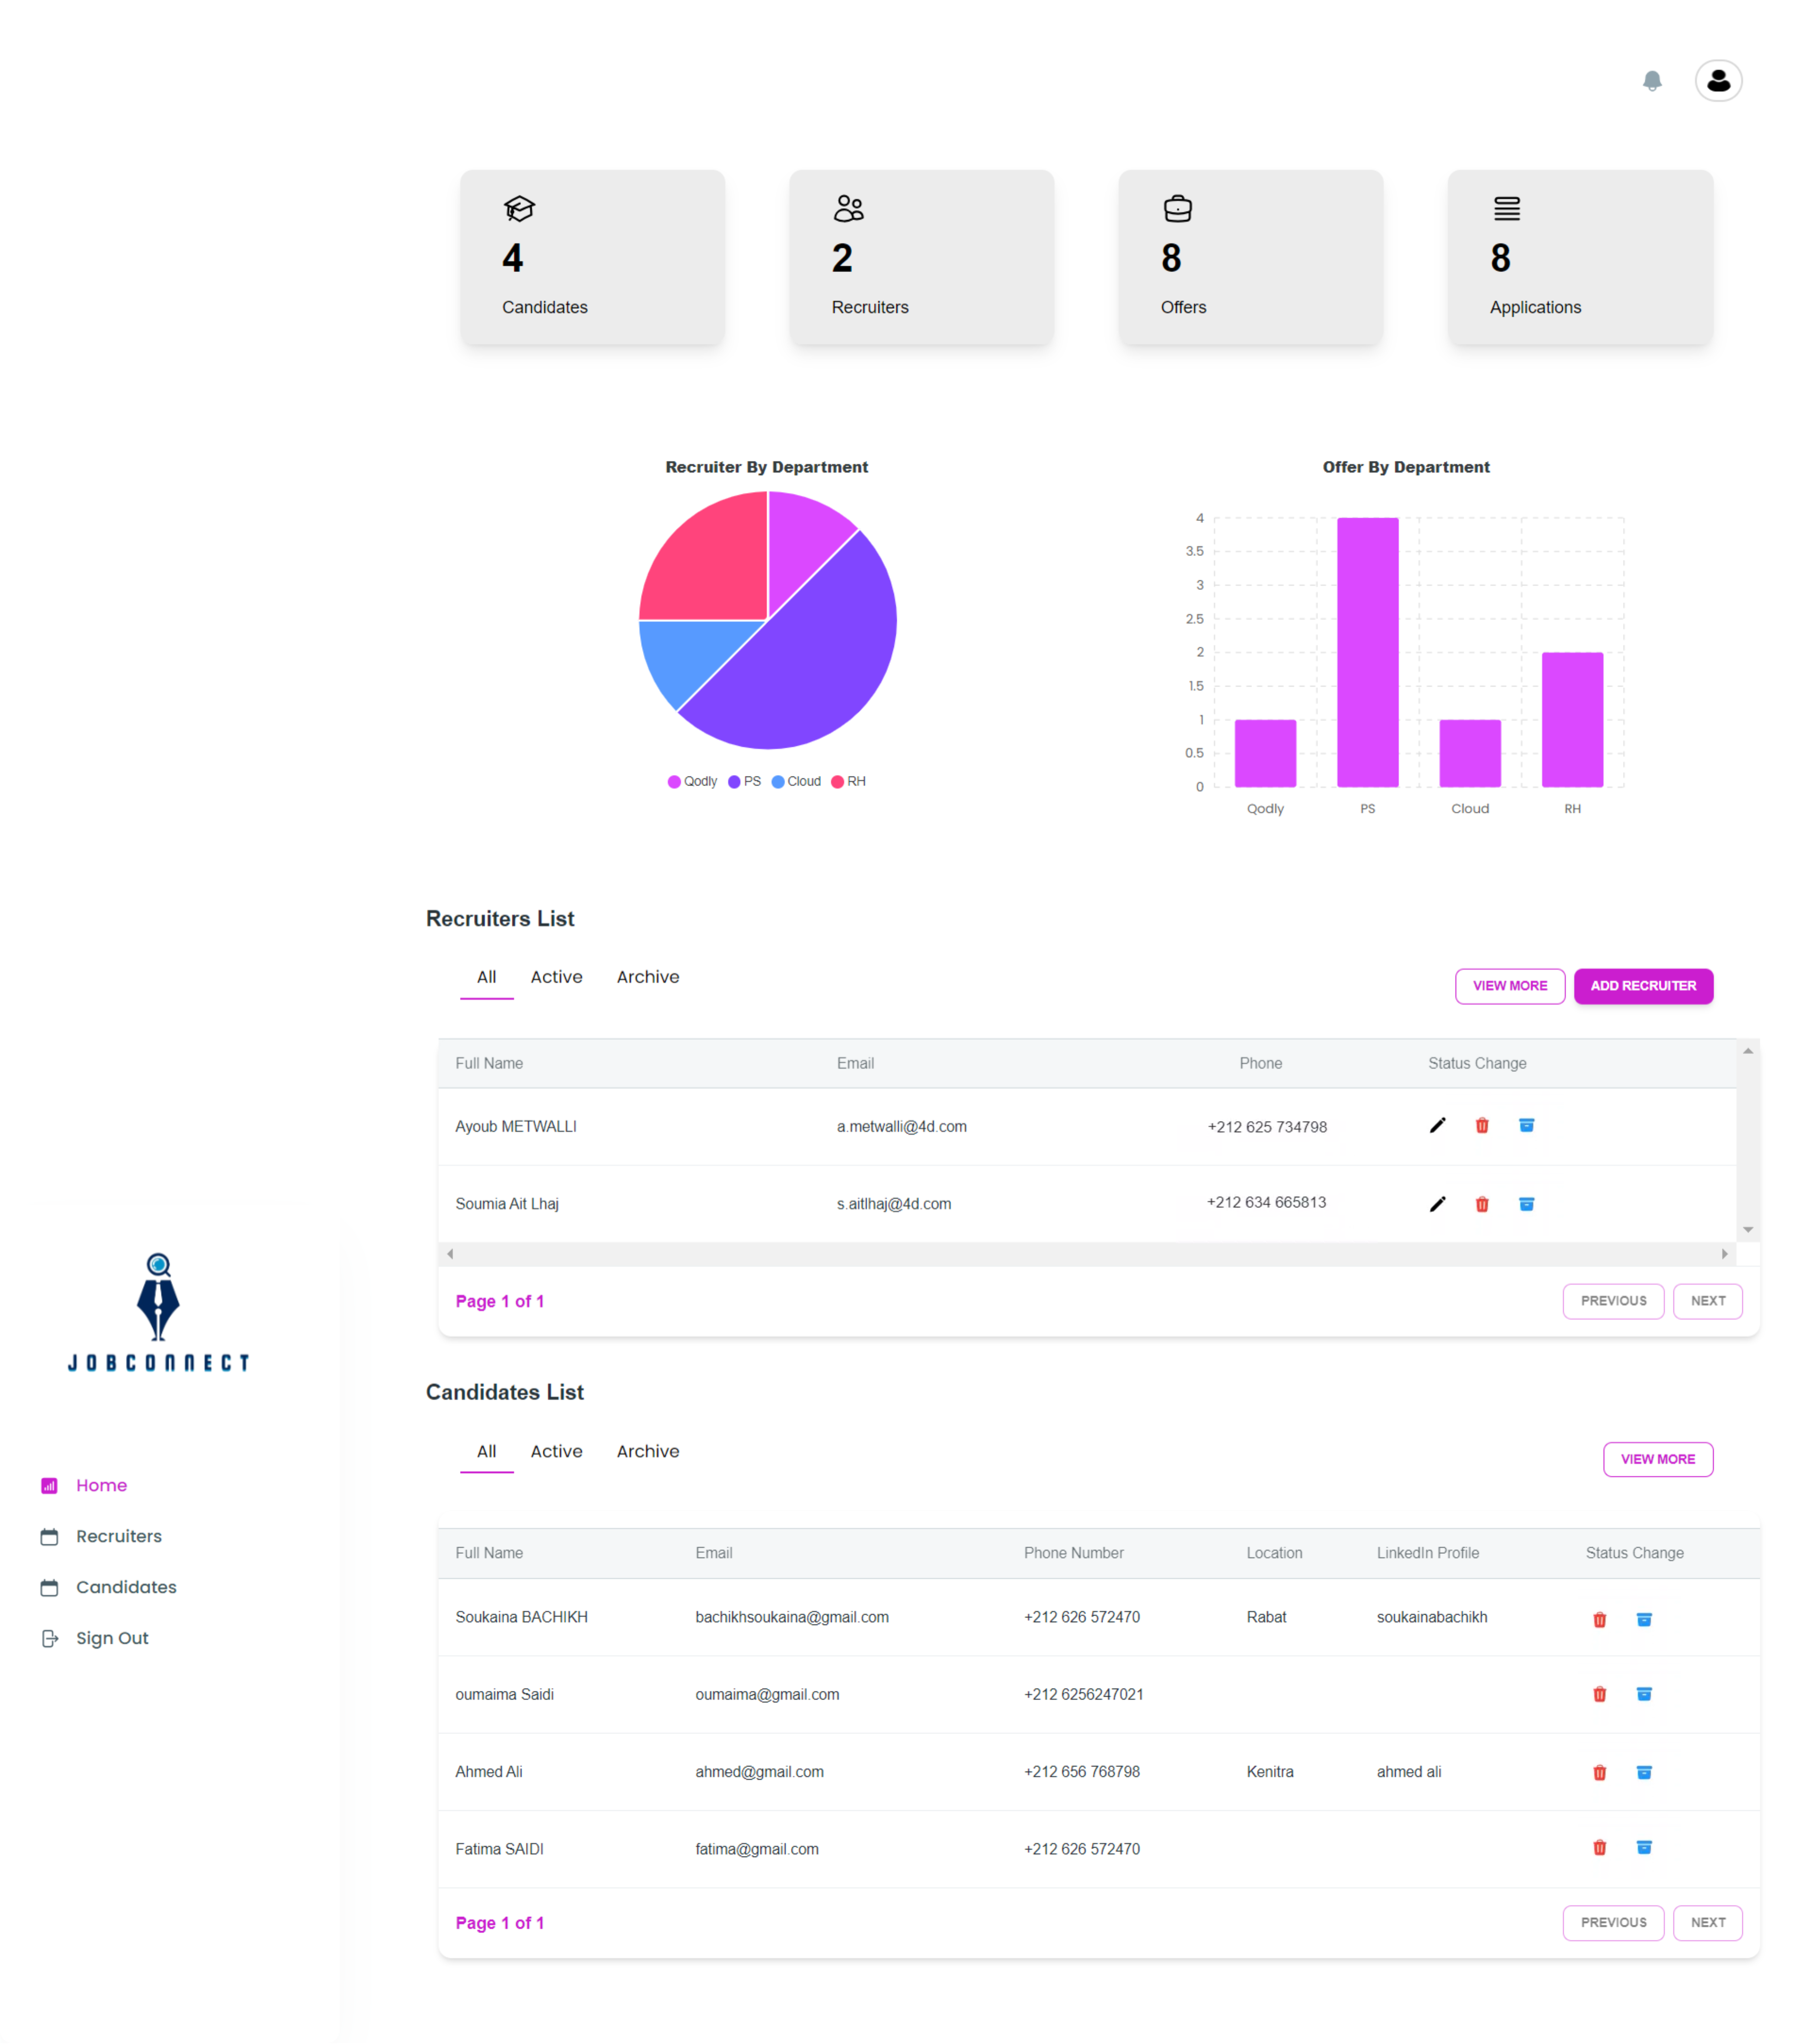
\includegraphics[scale=0.2]{screens/dashAdmin.png} 
   \caption{Le tableau de bord administratif}
   \label{fig:bordAdmin}
\end{figure}

\subsubsection{Archiver un candidat / un recruteur}

Permet à l'administrateur d'archiver un candidat ou un recruteur, assurant ainsi une gestion efficace de la base de données d'utilisateurs.


\subsubsection{Ajouter un recruteur}

Cette fonctionnalité permet à l'administrateur d'ajouter de nouveaux recruteurs à l'équipe de gestion des recrutements.
\begin{figure}[htbp]
   \centering
   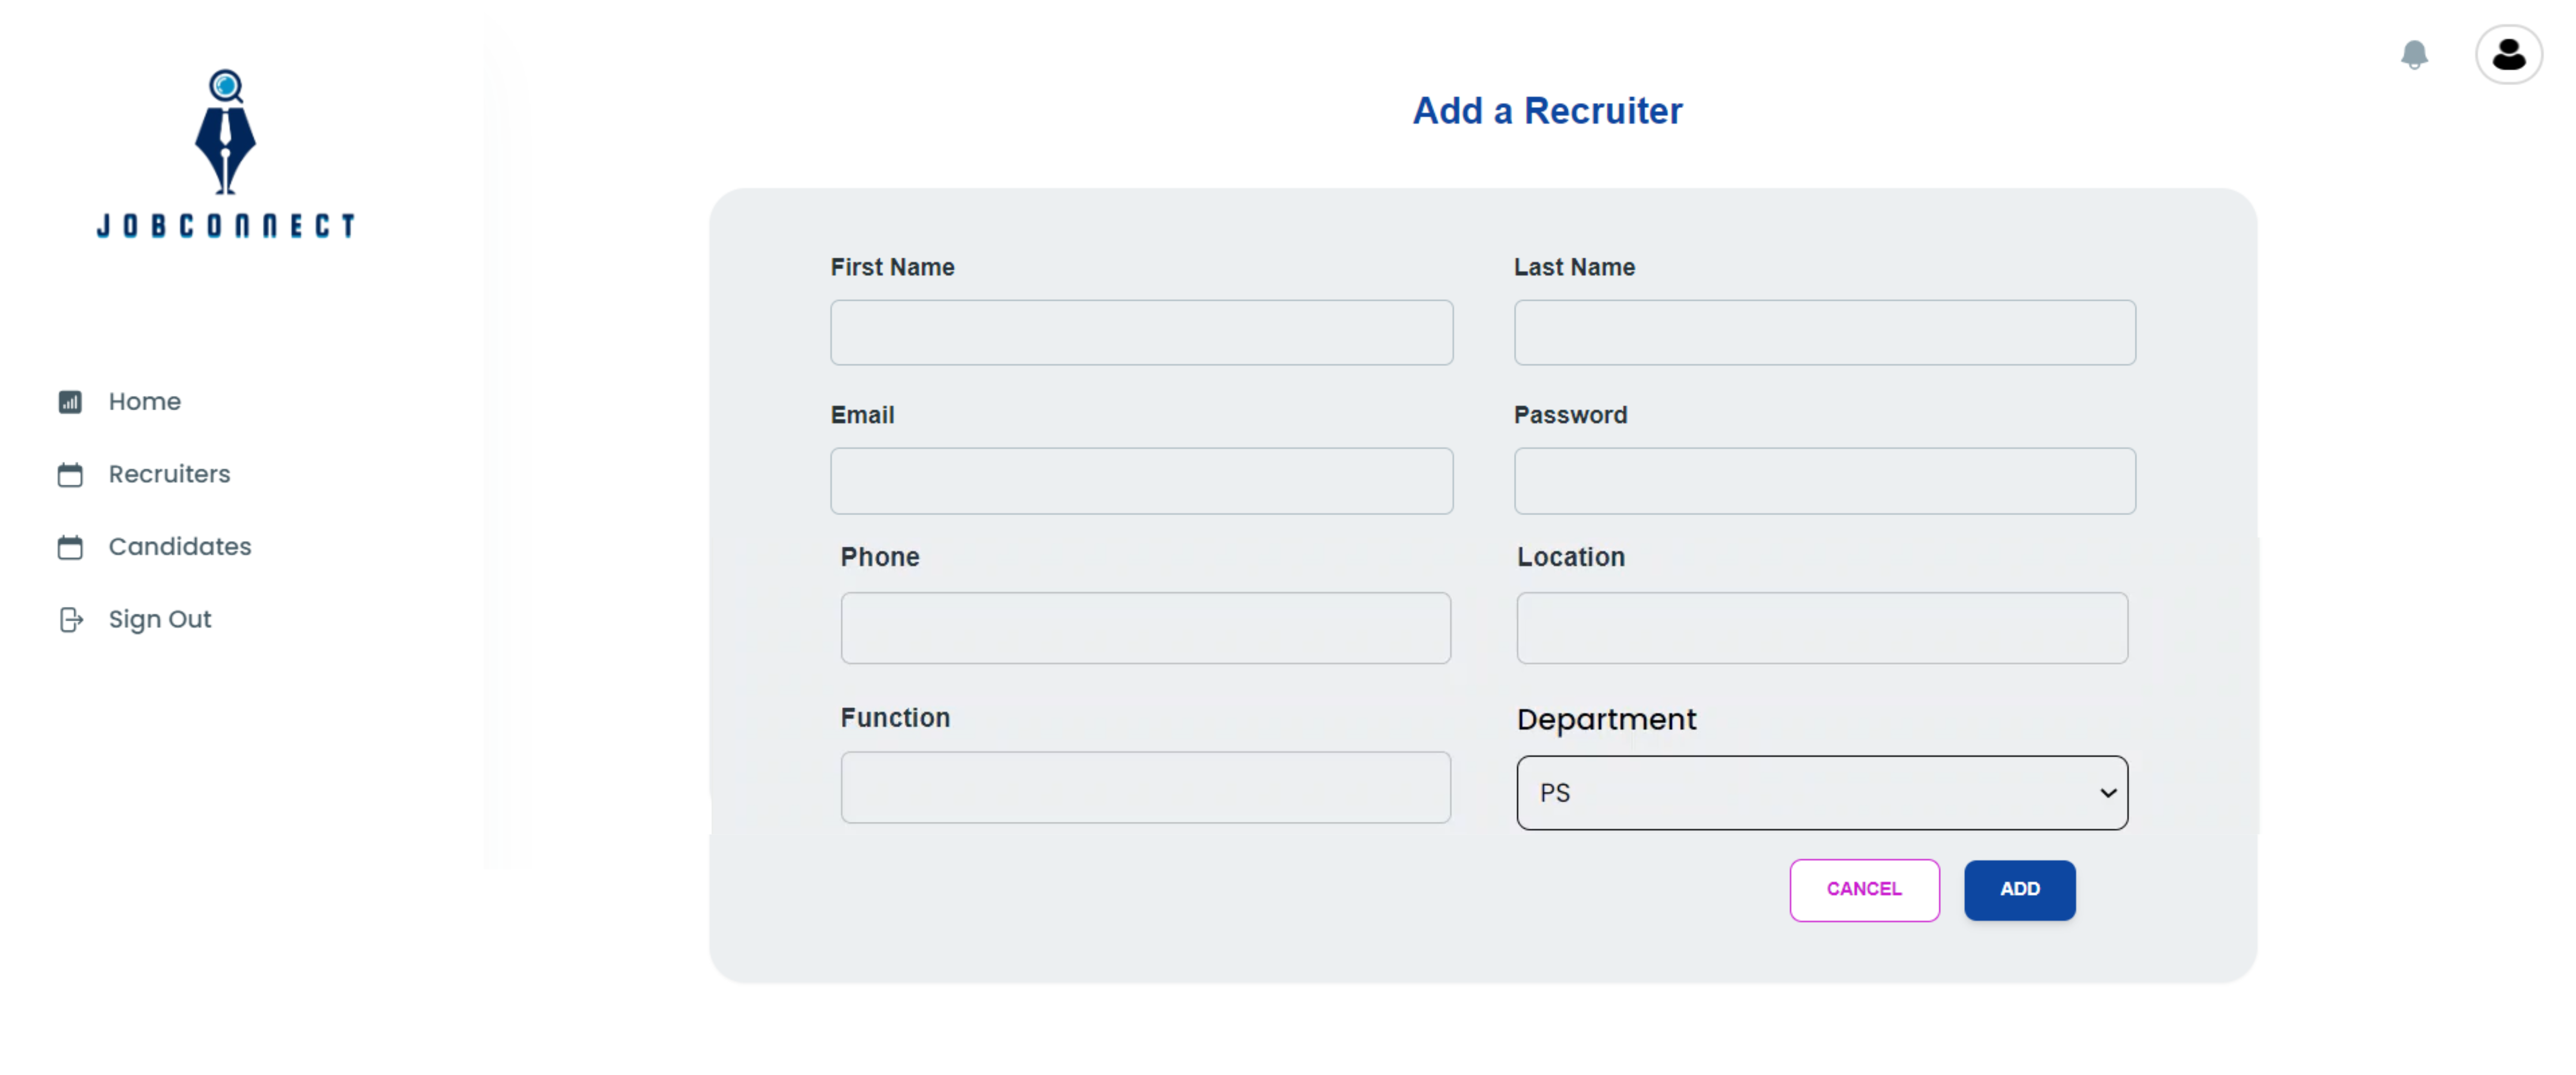
\includegraphics[scale=0.2]{screens/addRecruiter.png} 
   \caption{Ajouter un recruteur}
   \label{fig:addRec}
\end{figure}




\section{Test et Validation}
% \subsection{Tests unitaires}
% Jest

\subsection{Tests de bout en bout (E2E)}
\subsubsection{Définition et importance}

Dans le contexte de notre projet, le test end-to-end fait référence à une approche de test qui vise à évaluer le système dans son ensemble, en simulant les conditions réelles d’utilisation. Il s’agit d’un type de test qui vérifie le bon fonctionnement du système depuis le début jusqu’à la fin, en testant toutes les étapes intermédiaires et les  interactions entre les  composants. L’importance du test end-to-end dans notre projet réside dans sa capacité  à valider  la fonctionnalité globale du système et à identifier les problèmes d’intégration potentiels. En effectuant des tests end-to-end, vous pouvez vérifier si toutes les parties du système fonctionnent harmonieusement ensemble et satisfont les exigences spécifiées.
\newline

Ces tests permettent également d’évaluer  les  performances  du  système dans des scénarios réalistes, en tenant compte des conditions et des charges de travail typiques. Ils offrent une vision globale de la  qualité  du  système,  en mettant l’accent sur les fonctionnalités essentielles et les  cas  d’utilisation critiques pour les utilisateurs finaux. En résumé, le test end-to-end est essentiel dans votre projet pour s’assurer que toutes les parties du système fonctionnent correctement ensemble, répondent aux exigences et offrent une expérience utilisateur optimale. Il permet d’identifier et de résoudre les problèmes d’intégration pré- cocement, ce qui améliore la  qualité  du  produit  final.  La figure montre le fonctionnement du test E2E par cypress.
\begin{figure}[htbp]
   \centering
   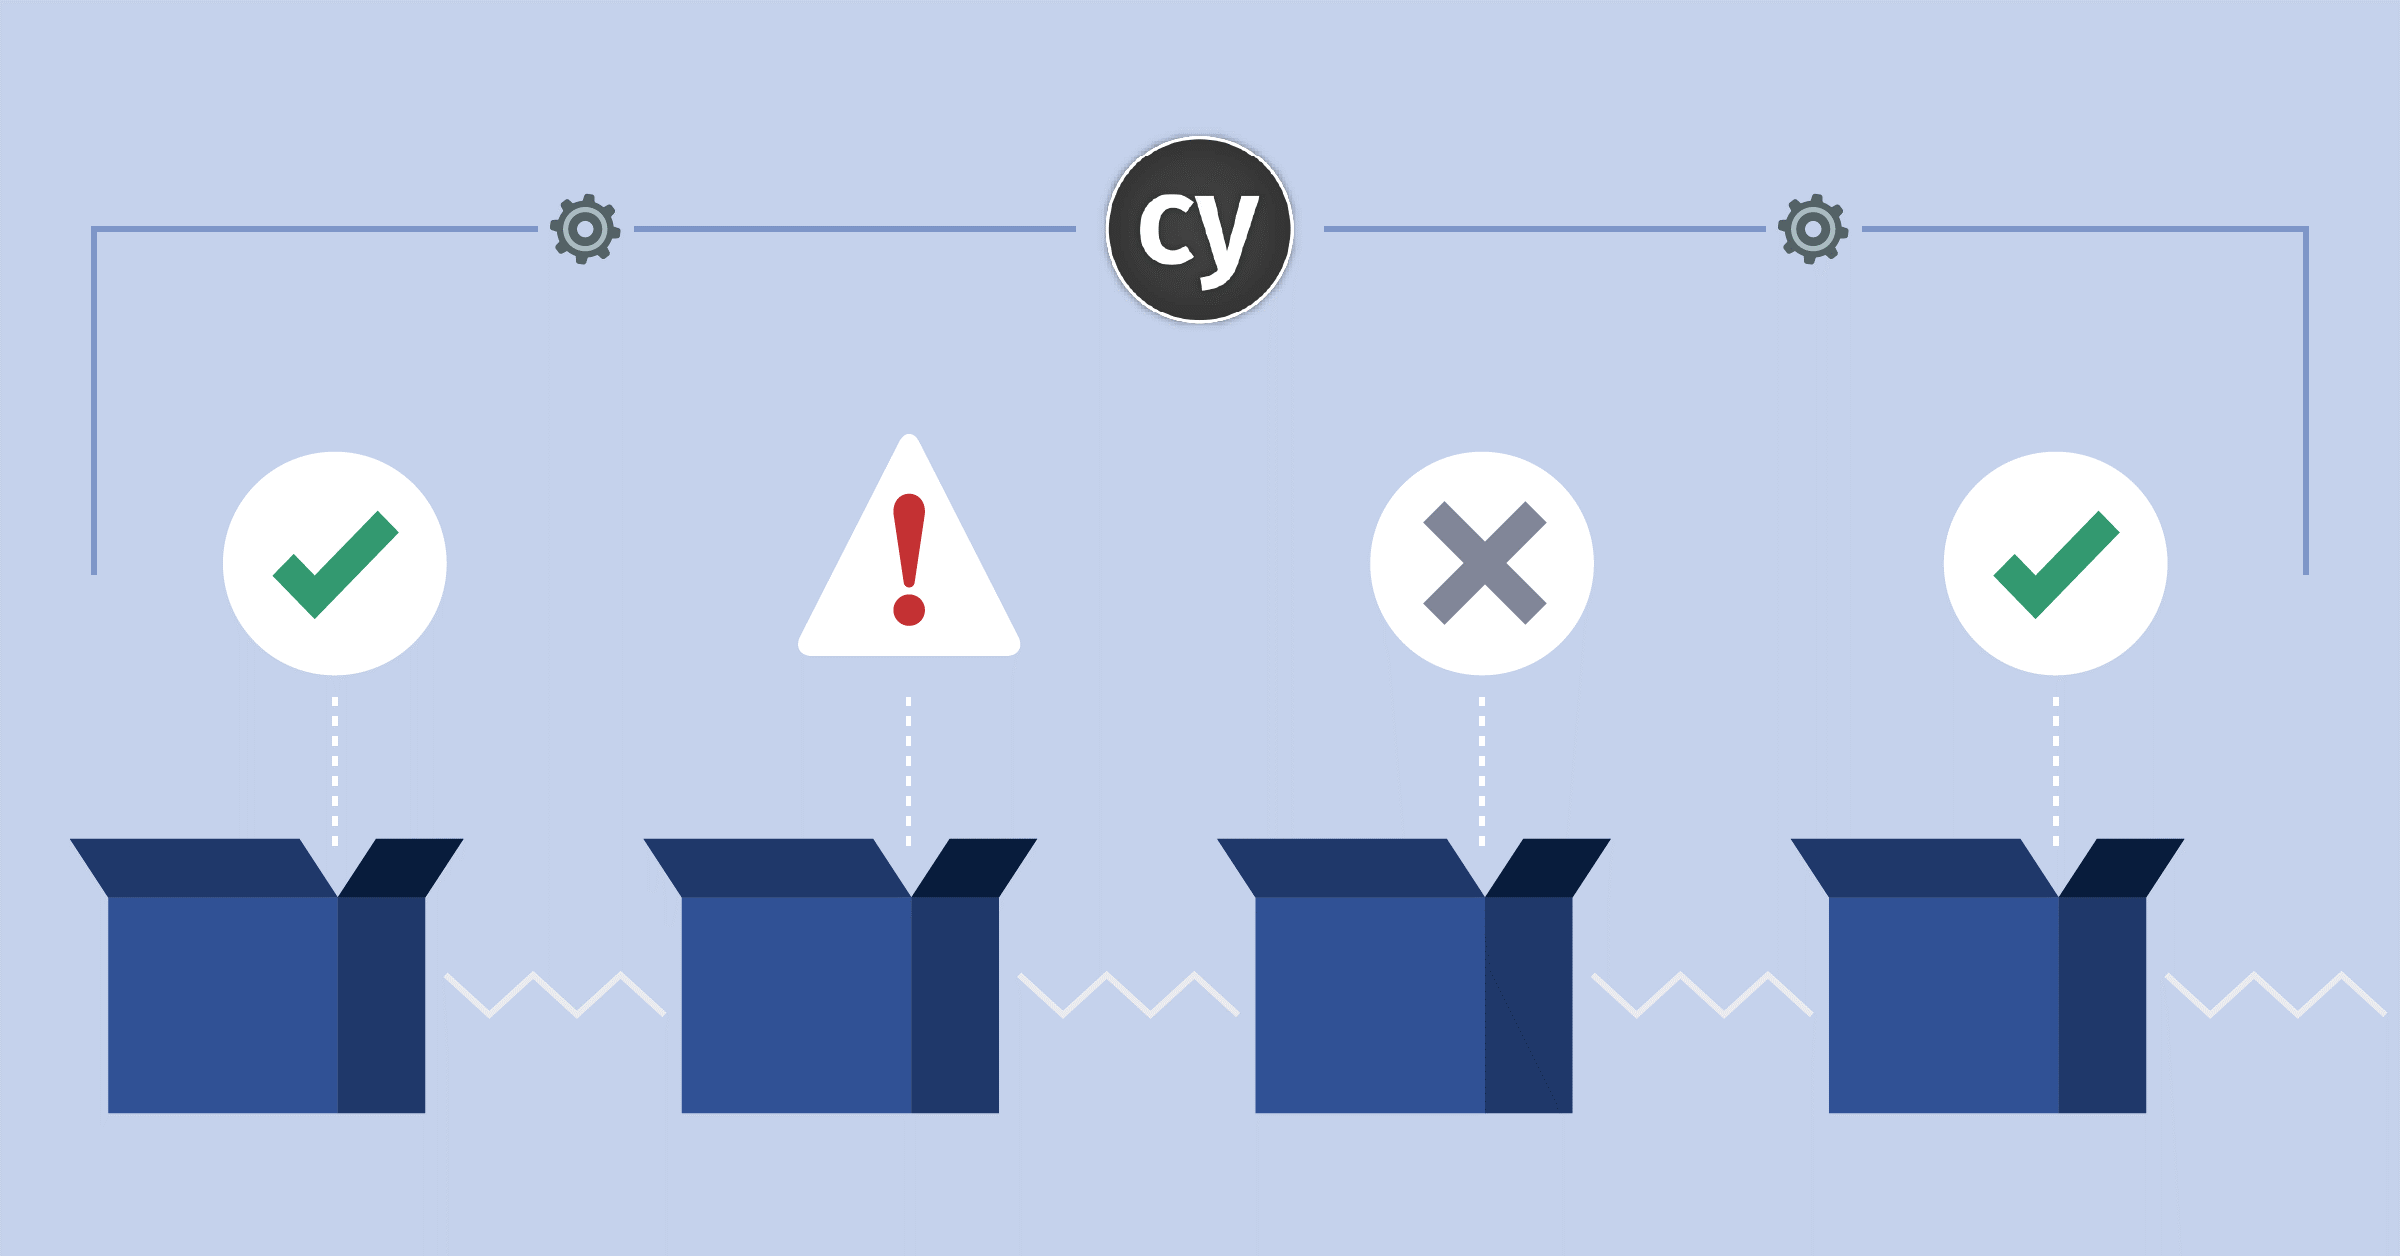
\includegraphics[scale=0.2]{cypress/1.png} 
   \caption{Fonctionnement du test End to End (E2E)}
   \label{fig:listOffers}
\end{figure}



\subsubsection{Exemple sur la page d’authentification}
Pour démarrer, exécutez la commande "npx cypress open" afin d'ouvrir la fenêtre de l'application Cypress sur la figure \ref{fig:cy1}.
\newline

\begin{figure}[htbp]
   \centering
   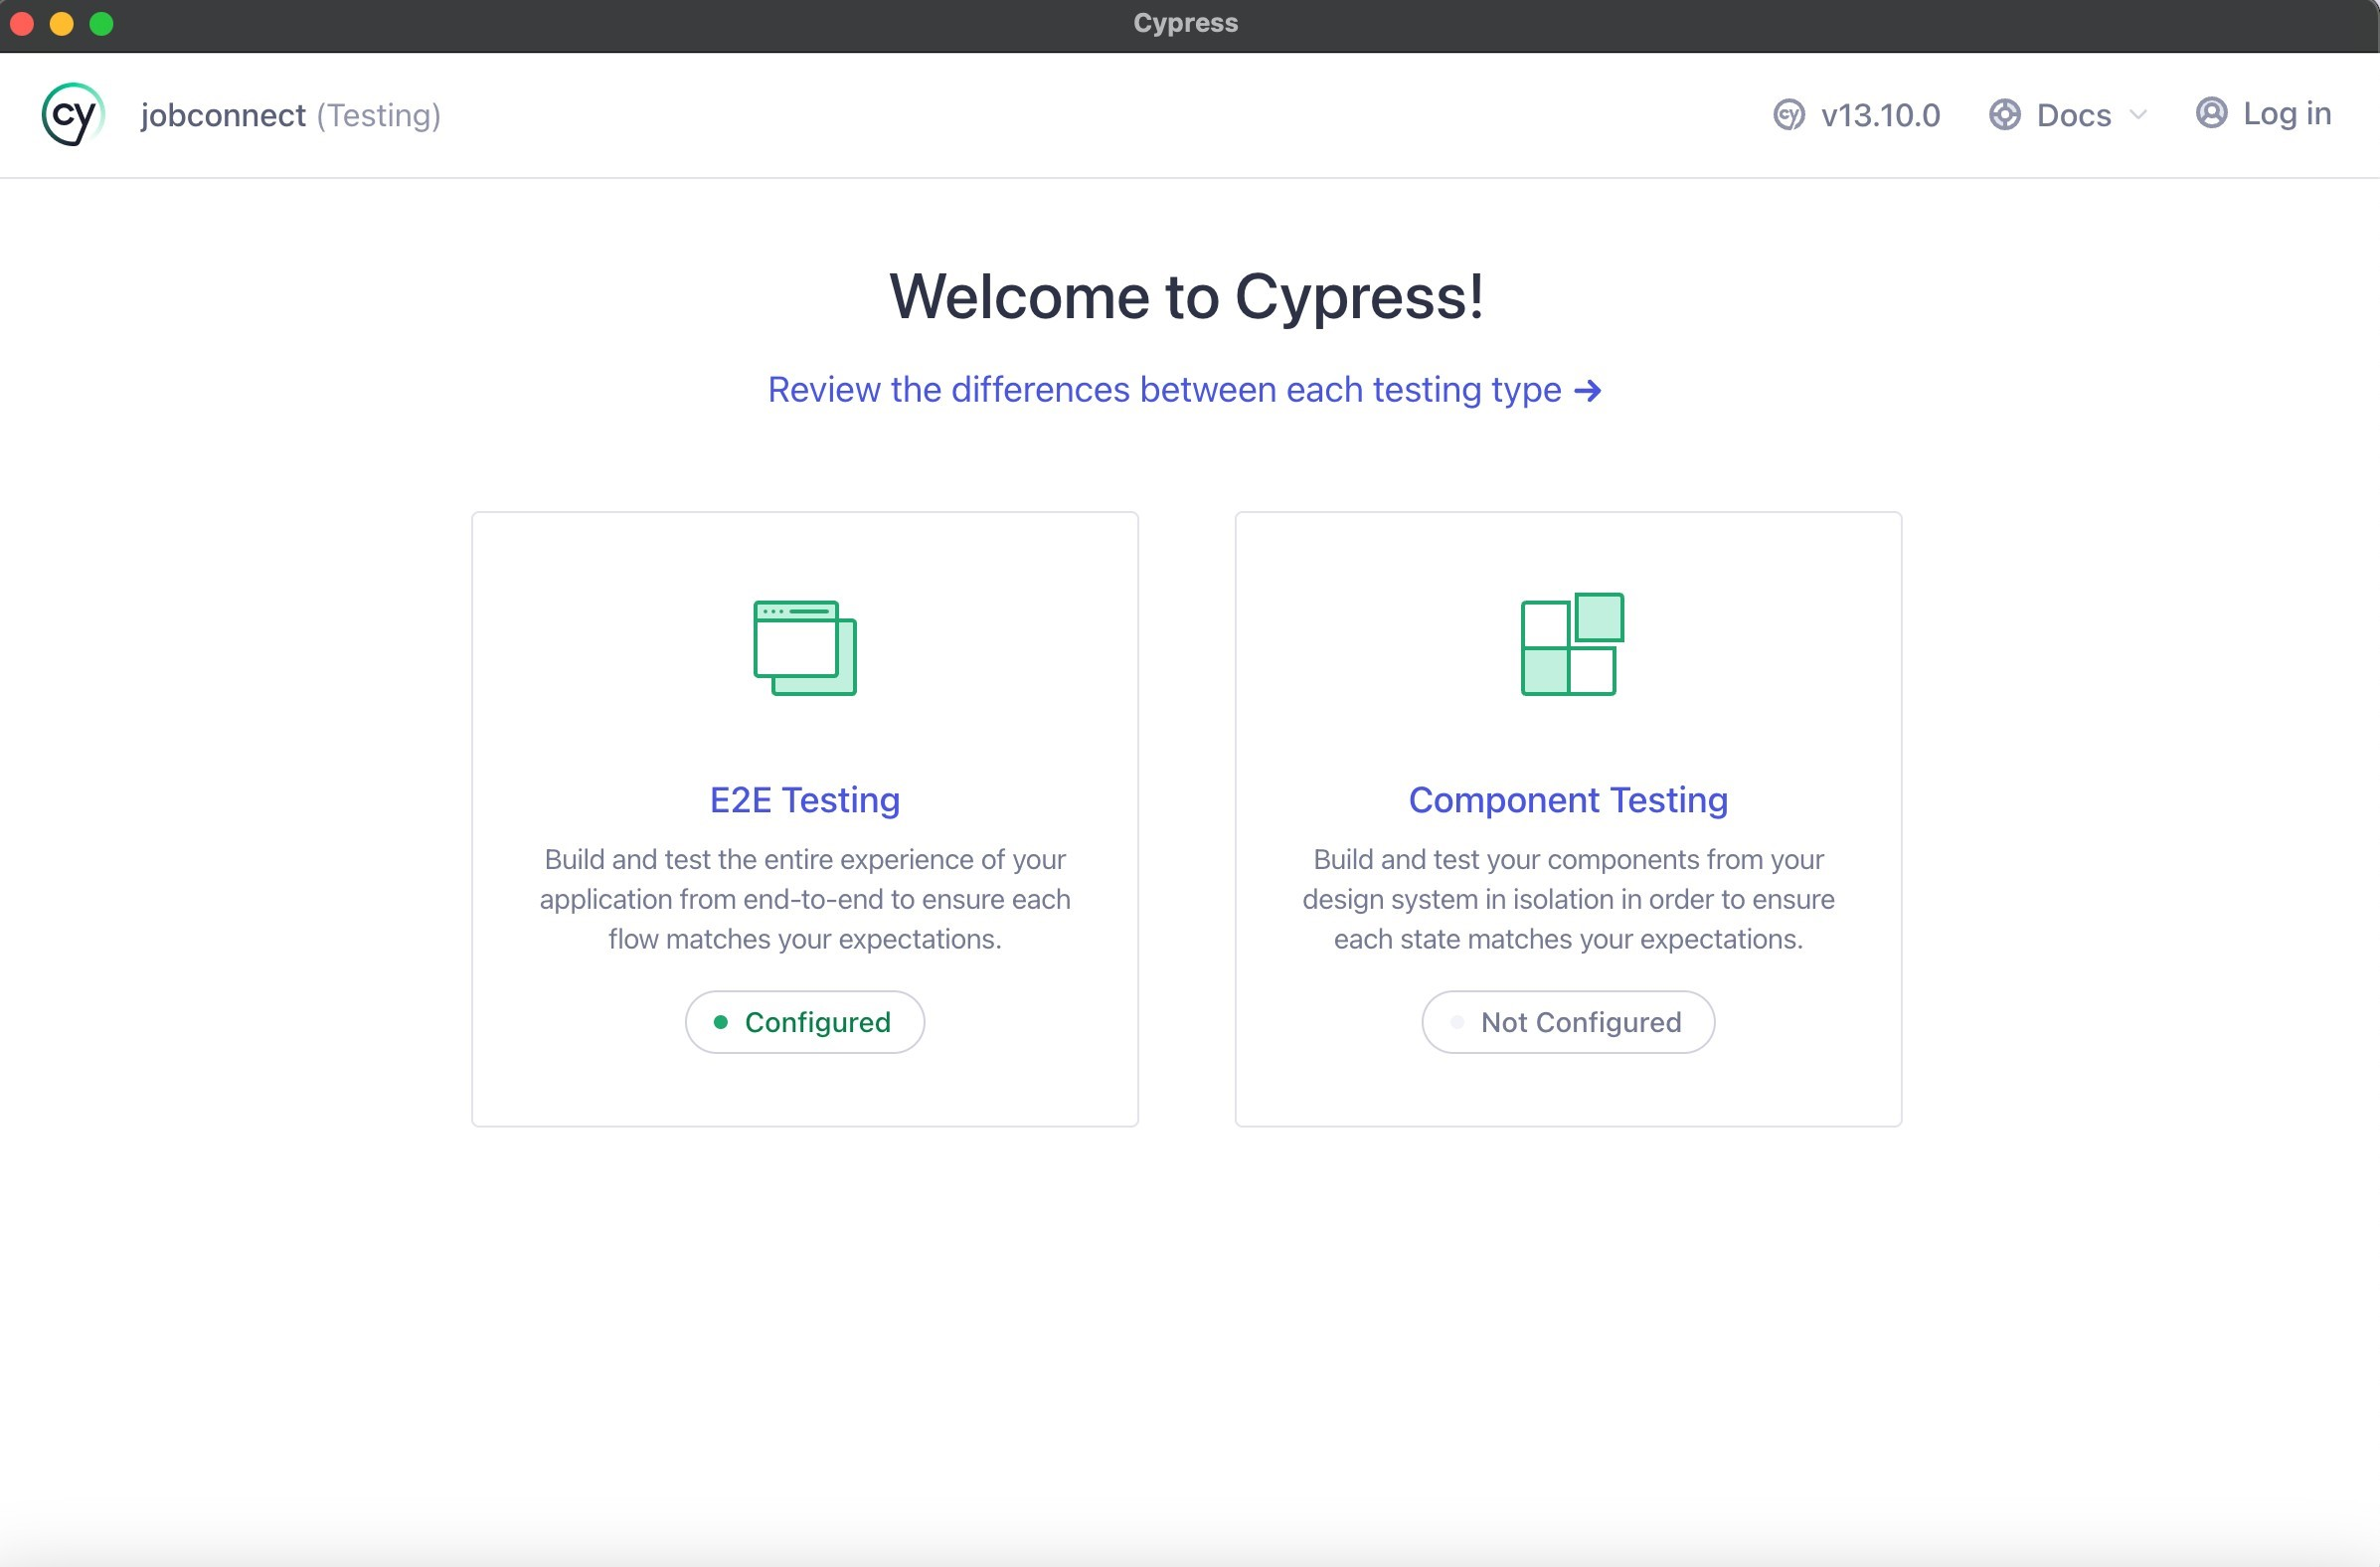
\includegraphics[scale=0.2]{cypress/2.jpg} 
   \caption{L'ouverture de Cypress}
   \label{fig:cy1}
\end{figure}

Une fois que vous avez ouvert Cypress, sélectionnez l’option de test E2E qui est déjà configurée. Ensuite, on choisit le navigateur sur lequel on souhaite exécuter nos tests, comme il est représenté sur la figure.
\\
\\
\\
\\
\\
\\

\begin{figure}[htbp]
   \centering
   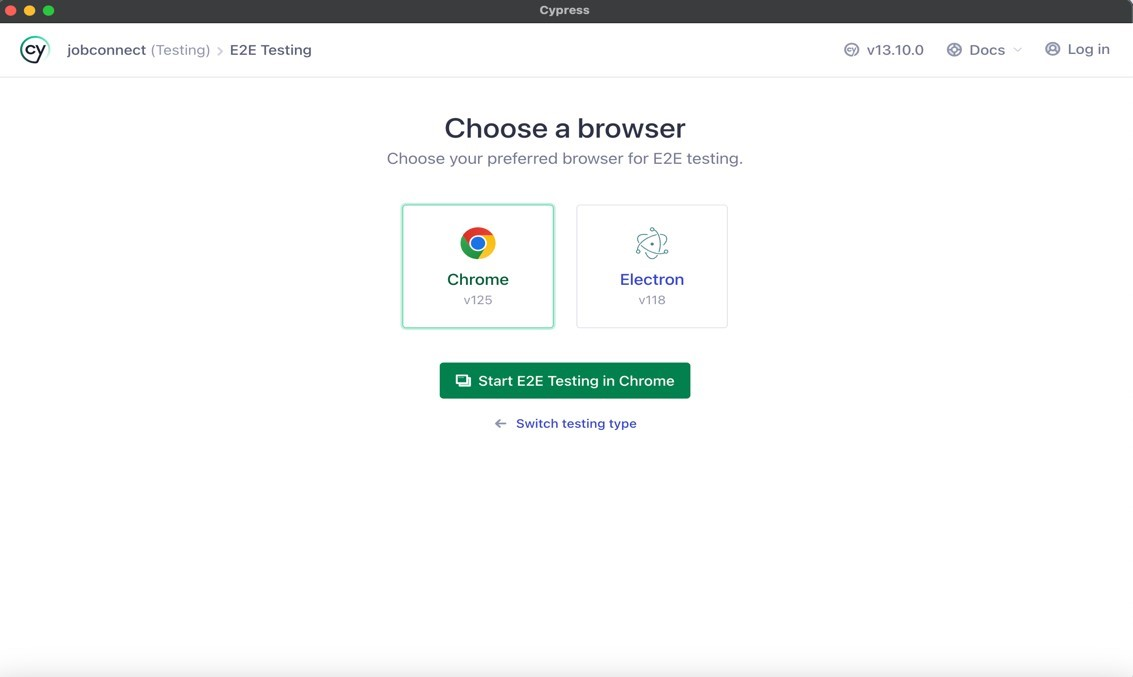
\includegraphics[scale=0.4]{cypress/3.jpg} 
   \caption{Choix de navigateur au niveau de Cypress}
   \label{fig:listOffers}
\end{figure}

Une fois le fichier "login.cy.jsx" (spec) créé, vous pouvez procéder à son test sur l'application, comme illustré dans la figure.
\newline

\begin{figure}[htbp]
   \centering
   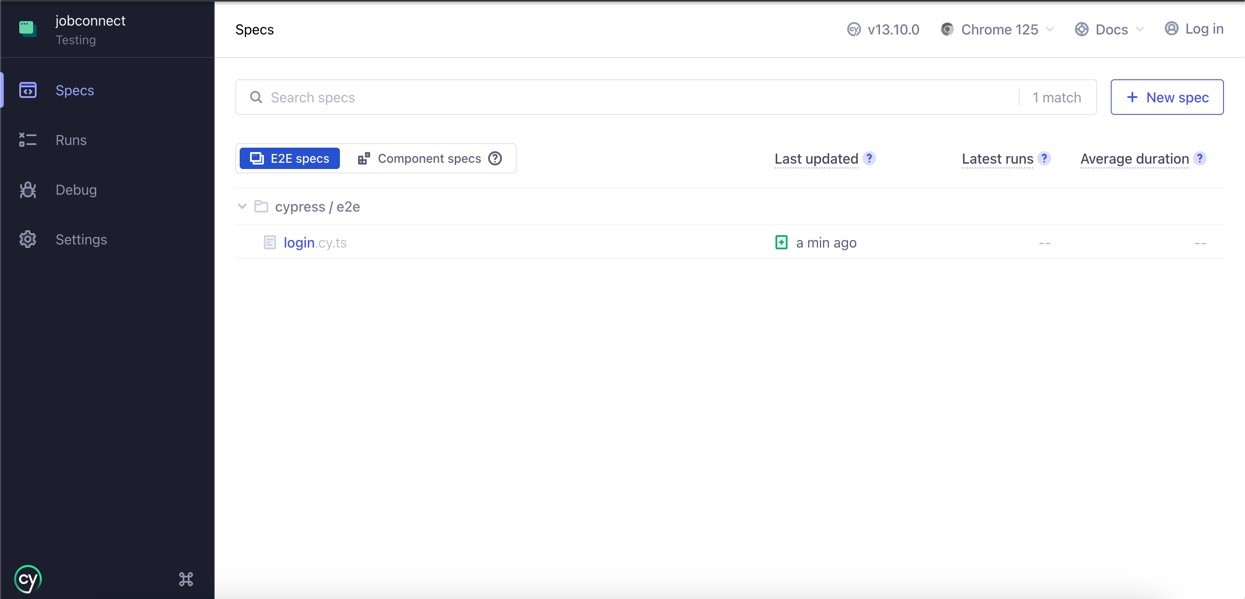
\includegraphics[scale=0.4]{cypress/4.jpg} 
   \caption{ End to End test avec Cypress}
   \label{fig:listOffers}
\end{figure}

Le résultat du test effectué sur notre page de connexion est sur la figure
\\
\\
\\
\begin{figure}[htbp]
   \centering
   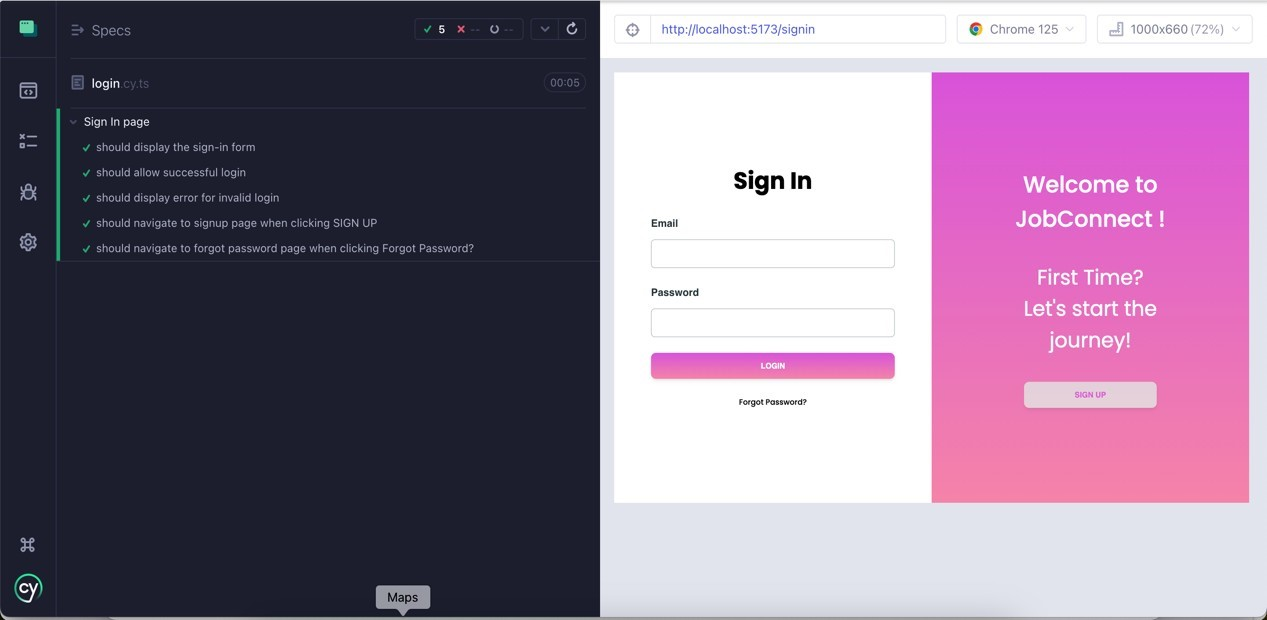
\includegraphics[scale=0.4]{cypress/5.jpg} 
   \caption{ Test End to End sur la page de login}
   \label{fig:listOffers}
\end{figure}

En résumé, Cypress facilite considérablement les étapes de création, d’exécution et de débogage des tests end-to-end. Il propose une approche conviviale et efficace pour garantir le bon fonctionnement global de notre application en simulant les interactions utilisateur réelles.


\section{Conclusion}
Cette partie du projet a présenté la mise en œuvre de l'application et  la  réalisation  des tests end-to-end. 
Nous avons présenté les différentes étapes de la mise en place de l'application et les différentes
technologies utilisées. Nous avons également présenté les différentes étapes de la réalisation des tests
end-to-end et les différentes technologies utilisées. 
\newline
